% A LaTeX template for MSc Thesis submissions to 
% Politecnico di Milano (PoliMi) - School of Industrial and Information Engineering
%
% S. Bonetti, A. Gruttadauria, G. Mescolini, A. Zingaro
% e-mail: template-tesi-ingind@polimi.it
%
% Last Revision: October 2021
%
% Copyright 2021 Politecnico di Milano, Italy. NC-BY

\documentclass{Configuration_Files/PoliMi3i_thesis}

%------------------------------------------------------------------------------
%	REQUIRED PACKAGES AND  CONFIGURATIONS
%------------------------------------------------------------------------------

% CONFIGURATIONS
\usepackage{parskip} % For paragraph layout
\usepackage{setspace} % For using single or double spacing
\usepackage{emptypage} % To insert empty pages
\usepackage{multicol} % To write in multiple columns (executive summary)
\setlength\columnsep{15pt} % Column separation in executive summary
\setlength\parindent{0pt} % Indentation
\raggedbottom  

% PACKAGES FOR TITLES
\usepackage{titlesec}
% \titlespacing{\section}{left spacing}{before spacing}{after spacing}
\titlespacing{\section}{0pt}{3.3ex}{2ex}
\titlespacing{\subsection}{0pt}{3.3ex}{1.65ex}
\titlespacing{\subsubsection}{0pt}{3.3ex}{1ex}
\usepackage{color}

% PACKAGES FOR LANGUAGE AND FONT
\usepackage[english]{babel} % The document is in English  
\usepackage[utf8]{inputenc} % UTF8 encoding
\usepackage[T1]{fontenc} % Font encoding
\usepackage[11pt]{moresize} % Big fonts

% PACKAGES FOR IMAGES
\usepackage{graphicx}
\usepackage{transparent} % Enables transparent images
\usepackage{eso-pic} % For the background picture on the title page
\usepackage{subfig} % Numbered and caption subfigures using \subfloat.
\usepackage{tikz} % A package for high-quality hand-made figures.
\usetikzlibrary{}
\graphicspath{{./Images/}} % Directory of the images
\usepackage{caption} % Coloured captions
\usepackage{xcolor} % Coloured captions
\usepackage{amsthm,thmtools,xcolor} % Coloured "Theorem"
\usepackage{float}

% STANDARD MATH PACKAGES
\usepackage{amsmath}
\usepackage{amsthm}
\usepackage{amssymb}
\usepackage{amsfonts}
\usepackage{bm}
\usepackage[overload]{empheq} % For braced-style systems of equations.
\usepackage{fix-cm} % To override original LaTeX restrictions on sizes

% PACKAGES FOR TABLES
\usepackage{tabularx}
\usepackage{longtable} % Tables that can span several pages
\usepackage{colortbl}

% PACKAGES FOR ALGORITHMS (PSEUDO-CODE)
\usepackage{algorithm}
\usepackage{algorithmic}

% PACKAGES FOR REFERENCES & BIBLIOGRAPHY
\usepackage[colorlinks=true,linkcolor=black,anchorcolor=black,citecolor=black,filecolor=black,menucolor=black,runcolor=black,urlcolor=black]{hyperref} % Adds clickable links at references
\usepackage{cleveref}
\usepackage[square, numbers, sort&compress]{natbib} % Square brackets, citing references with numbers, citations sorted by the appearance in the text and compressed
\bibliographystyle{unsrt} % You may use a different style adapted to your field

% OTHER PACKAGES
\usepackage{pdfpages} % To include a pdf file
\usepackage{afterpage}
\usepackage{lipsum} % DUMMY PACKAGE
\usepackage{fancyhdr} % For the headers
\fancyhf{}

% Input of configuration file. Do not change config.tex file unless you really know what you are doing. 
% Define blue color typical of polimi
\definecolor{bluepoli}{cmyk}{0.4,0.1,0,0.4}

% Custom theorem environments
\declaretheoremstyle[
  headfont=\color{bluepoli}\normalfont\bfseries,
  bodyfont=\color{black}\normalfont\itshape,
]{colored}

% Set-up caption colors
\captionsetup[figure]{labelfont={color=bluepoli}} % Set colour of the captions
\captionsetup[table]{labelfont={color=bluepoli}} % Set colour of the captions

\theoremstyle{colored}
\newtheorem{theorem}{Theorem}[chapter]
\newtheorem{proposition}{Proposition}[chapter]

% Enhances the features of the standard "table" and "tabular" environments.
\newcommand\T{\rule{0pt}{2.6ex}}
\newcommand\B{\rule[-1.2ex]{0pt}{0pt}}

% Pseudo-code algorithm descriptions.
\newcounter{algsubstate}
\renewcommand{\thealgsubstate}{\alph{algsubstate}}
\newenvironment{algsubstates}
  {\setcounter{algsubstate}{0}%
   \renewcommand{\STATE}{%
     \stepcounter{algsubstate}%
     \Statex {\small\thealgsubstate:}\space}}
  {}

% New font size
\newcommand\numfontsize{\@setfontsize\Huge{200}{60}}

% Title format: chapter
\titleformat{\chapter}[hang]{
\fontsize{50}{20}\selectfont\bfseries\filright}{\textcolor{bluepoli} \thechapter\hsp\hspace{2mm}\textcolor{bluepoli}{|   }\hsp}{0pt}{\huge\bfseries \textcolor{bluepoli}
}

% Title format: section
\titleformat{\section}
{\color{bluepoli}\normalfont\Large\bfseries}
{\color{bluepoli}\thesection.}{1em}{}

% Title format: subsection
\titleformat{\subsection}
{\color{bluepoli}\normalfont\large\bfseries}
{\color{bluepoli}\thesubsection.}{1em}{}

% Title format: subsubsection
\titleformat{\subsubsection}
{\color{bluepoli}\normalfont\large\bfseries}
{\color{bluepoli}\thesubsubsection.}{1em}{}

% Shortening for setting no horizontal-spacing
\newcommand{\hsp}{\hspace{0pt}}

\makeatletter
% Renewcommand: cleardoublepage including the background pic
\renewcommand*\cleardoublepage{%
  \clearpage\if@twoside\ifodd\c@page\else
  \null
  \AddToShipoutPicture*{\BackgroundPic}
  \thispagestyle{empty}%
  \newpage
  \if@twocolumn\hbox{}\newpage\fi\fi\fi}
\makeatother

%For correctly numbering algorithms
\numberwithin{algorithm}{chapter}

%----------------------------------------------------------------------------
%	NEW COMMANDS DEFINED
%----------------------------------------------------------------------------

% EXAMPLES OF NEW COMMANDS
\newcommand{\bea}{\begin{eqnarray}} % Shortcut for equation arrays
\newcommand{\eea}{\end{eqnarray}}
\newcommand{\e}[1]{\times 10^{#1}}  % Powers of 10 notation

%----------------------------------------------------------------------------
%	ADD YOUR PACKAGES (be careful of package interaction)
%----------------------------------------------------------------------------

%----------------------------------------------------------------------------
%	ADD YOUR DEFINITIONS AND COMMANDS (be careful of existing commands)
%----------------------------------------------------------------------------

%----------------------------------------------------------------------------
%	BEGIN OF YOUR DOCUMENT
%----------------------------------------------------------------------------

\begin{document}

\fancypagestyle{plain}{%
\fancyhf{} % Clear all header and footer fields
\fancyhead[RO,RE]{\thepage} %RO=right odd, RE=right even
\renewcommand{\headrulewidth}{0pt}
\renewcommand{\footrulewidth}{0pt}}

%----------------------------------------------------------------------------
%	TITLE PAGE
%----------------------------------------------------------------------------

\pagestyle{empty} % No page numbers
\frontmatter % Use roman page numbering style (i, ii, iii, iv...) for the preamble pages

\puttitle{
	title=A comparison of ML models for \\ musical genre classification, % Title of the thesis
	name=Alberto Pirillo, % Author Name and Surname
	course=Numerical Analysis for Machine Learning \\ Computer Science and Engineering, % Study Programme (in Italian)
	advisor=Prof. Edie Miglio, % Advisor name
	academicyear={2022-2023},  % Academic Year
} % These info will be put into your Title page 

%----------------------------------------------------------------------------
%	PREAMBLE PAGES: ABSTRACT (inglese e italiano), EXECUTIVE SUMMARY
%----------------------------------------------------------------------------
\startpreamble
\setcounter{page}{1} % Set page counter to 1

%----------------------------------------------------------------------------
%	LIST OF CONTENTS/FIGURES/TABLES/SYMBOLS
%----------------------------------------------------------------------------

% TABLE OF CONTENTS
\thispagestyle{empty}
\tableofcontents % Table of contents 
\thispagestyle{empty}
\cleardoublepage

%-------------------------------------------------------------------------
%	THESIS MAIN TEXT
%-------------------------------------------------------------------------

\addtocontents{toc}{\vspace{2em}} % Add a gap in the Contents, for aesthetics
\mainmatter % Begin numeric (1,2,3...) page numbering

\chapter*{Introduction}
\label{ch:introduction}%
The goal of this project is to recreate and explore further the study on the automatic classification of musical genres originally proposed in the paper \textit{Classification of musical genre: a machine learning approach} \cite{original-paper}.

The analysis was recreated using a different data set, the \href{https://www.kaggle.com/data sets/andradaolteanu/gtzan-data set-music-genre-classification?resource=download-directory}{GTZAN data set} \cite{gtzan}.

Furthermore, given that Java is no longer the language of choice for machine learning applications, this work will rely on the Python programming language, and in particular mostly on the libraries \textit{scikit-learn} \cite{scikit-learn} and \textit{keras} \cite{chollet2015keras}, which are among the most popular ML/DL Python libraries at the moment of writing.

\section*{Data set}
\label{sec:dataset}%
The GTZAN data set is the most used public data set for evaluation in machine listening research for music genre recognition. The files were collected in 2000-2001 from a variety of sources including personal CDs, radio, and microphone recordings, in order to represent a variety of recording conditions.

The data set consists of a collection of 10 genres (blues, classical, country, disco, hip-hop, jazz, metal, pop, reggae and rock) with 100 audio files each, all having a length of 30 seconds. This means that the original data set is composed of just $1000$ samples. In order to increase the amount of data at our disposal, we split each song into 10 tracks each one with a length of 3 seconds. In this way, we are able to work with $10000$ samples. This is beneficial since it is known that a larger number of samples helps improve the performance of our model. 

It is worth noting that this splitting has some drawbacks since we are introducing some dependency among the samples, given that many samples were coming from the same song. However, we will neglect this aspect in our analysis since increasing the number of samples brings more significant benefits w.r.t. the disadvantages introduced by this correlation.

In our analysis, we will consider the file \textit{features\_3\_sec.csv} available in the data set. This file has an entry for each one of the tracks of 3 seconds we will consider. For each track, it contains the mean and the variance of a list of features extracted from the corresponding audio file.


\section*{Problem description}
\label{sec:problem_desc}
Supervised classification is one of the core tasks solved by Machine Learning.

Following the lead of the paper \cite{original-paper}, two categorization models were studied:
\begin{itemize}
    \item Multi-class classification: we are considering all the samples and all the musical genres at the same time. Our goal is to assign each one of the samples to one of the genres.
    \item Binary classification: we are considering the problem of determining whether a single sample belongs or not to a given genre, therefore we are considering only one genre at a time. We will need to train multiple independent models (one for each genre) considering only a subset of the samples. This is because in classification problems it is a good practice to have a balanced amount of data between the classes. Each model was trained considering all the samples of the corresponding genre and an equivalent amount of samples randomly selected from the other classes.
\end{itemize}

The most common metrics used in classification problems are accuracy, precision and recall. In order to evaluate the performance of the classification models, we will use accuracy. This is in order to be coherent with the original paper, and potentially to compare our results with theirs. 


\section*{Project steps}
\label{sec:steps}
As in any other data science work, the investigation begins with an Exploratory Data Analysis (EDA) to study the information contained in the GTZAN data set. It is covered in Chapter \ref{ch:eda}.

Then, following the example of the original paper \cite{original-paper}, we trained multiple machine learning models and evaluated their performance using both static partitioning (i.e. train-validation split) and dynamic partitioning (i.e. K-fold cross-validation).
Machine learning models are covered in Chapter \ref{ch:ml_models}

Finally, it was decided to tackle the problem using a more complex and more modern model not present in the original paper: feed-forward fully-connected neural networks. This is covered in Chapter \ref{ch:dl_models}.

A comparison between the performance of all those models is then presented in Chapter \ref{ch:comparison}.


All materials related to this project, including the source code, the final models, and the data that was stored in the database, are available in the project's GitHub repository \cite{project-repository}.

% --------------------------------------------------------------------------
% NUMBERED CHAPTERS % Regular chapters following
% --------------------------------------------------------------------------

\chapter{Exploratory Data Analysis}
\label{ch:eda}%
The analysis was conducted in a \href{https://jupyter.org/}{\textit{Jupyter Notebook}}, relying on the \href{https://pypi.org/project/pandas/}{\textit{pandas}} library for data manipulation and on the \href{https://pypi.org/project/matplotlib/}{\textit{matplotlib}} and \href{https://pypi.org/project/seaborn/}{\textit{seaborn}} libraries for data visualization. 

The goals of this EDA are the following:
\begin{itemize}
    \item Look for missing values and inconsistencies
    \item Find the most suitable data types
    \item Perform a correlation analysis to understand how to predict the label
    \item Visualize the data through the use of Principal Component Analysis (PCA)
\end{itemize}

The first step was checking for missing or duplicate data inside the data set.  \\
Neither missing nor duplicate data was found.

Then, the target variable, i.e. the musical genre of the songs, was studied. It can only assume 10 different values, which are the 10 musical genres we are considering. This means that the target variable is a categorical variable. We can also observe that the classes are only slightly imbalanced w.r.t. one another, therefore we do not expect this to be an issue in the training of the models.

\section{Setting data types}
\label{sec:datatypes}%
The data types automatically inferred by \textit{pandas} are known to be sub-optimal. In order to use the least amount of memory possible, an analysis of the values taken by each feature was conducted.
In particular, the absolute value of the maximum value and of the minimum value of each numerical variable was plotted, as shown in the bar plot below.

\begin{figure}[H]
    \centering
    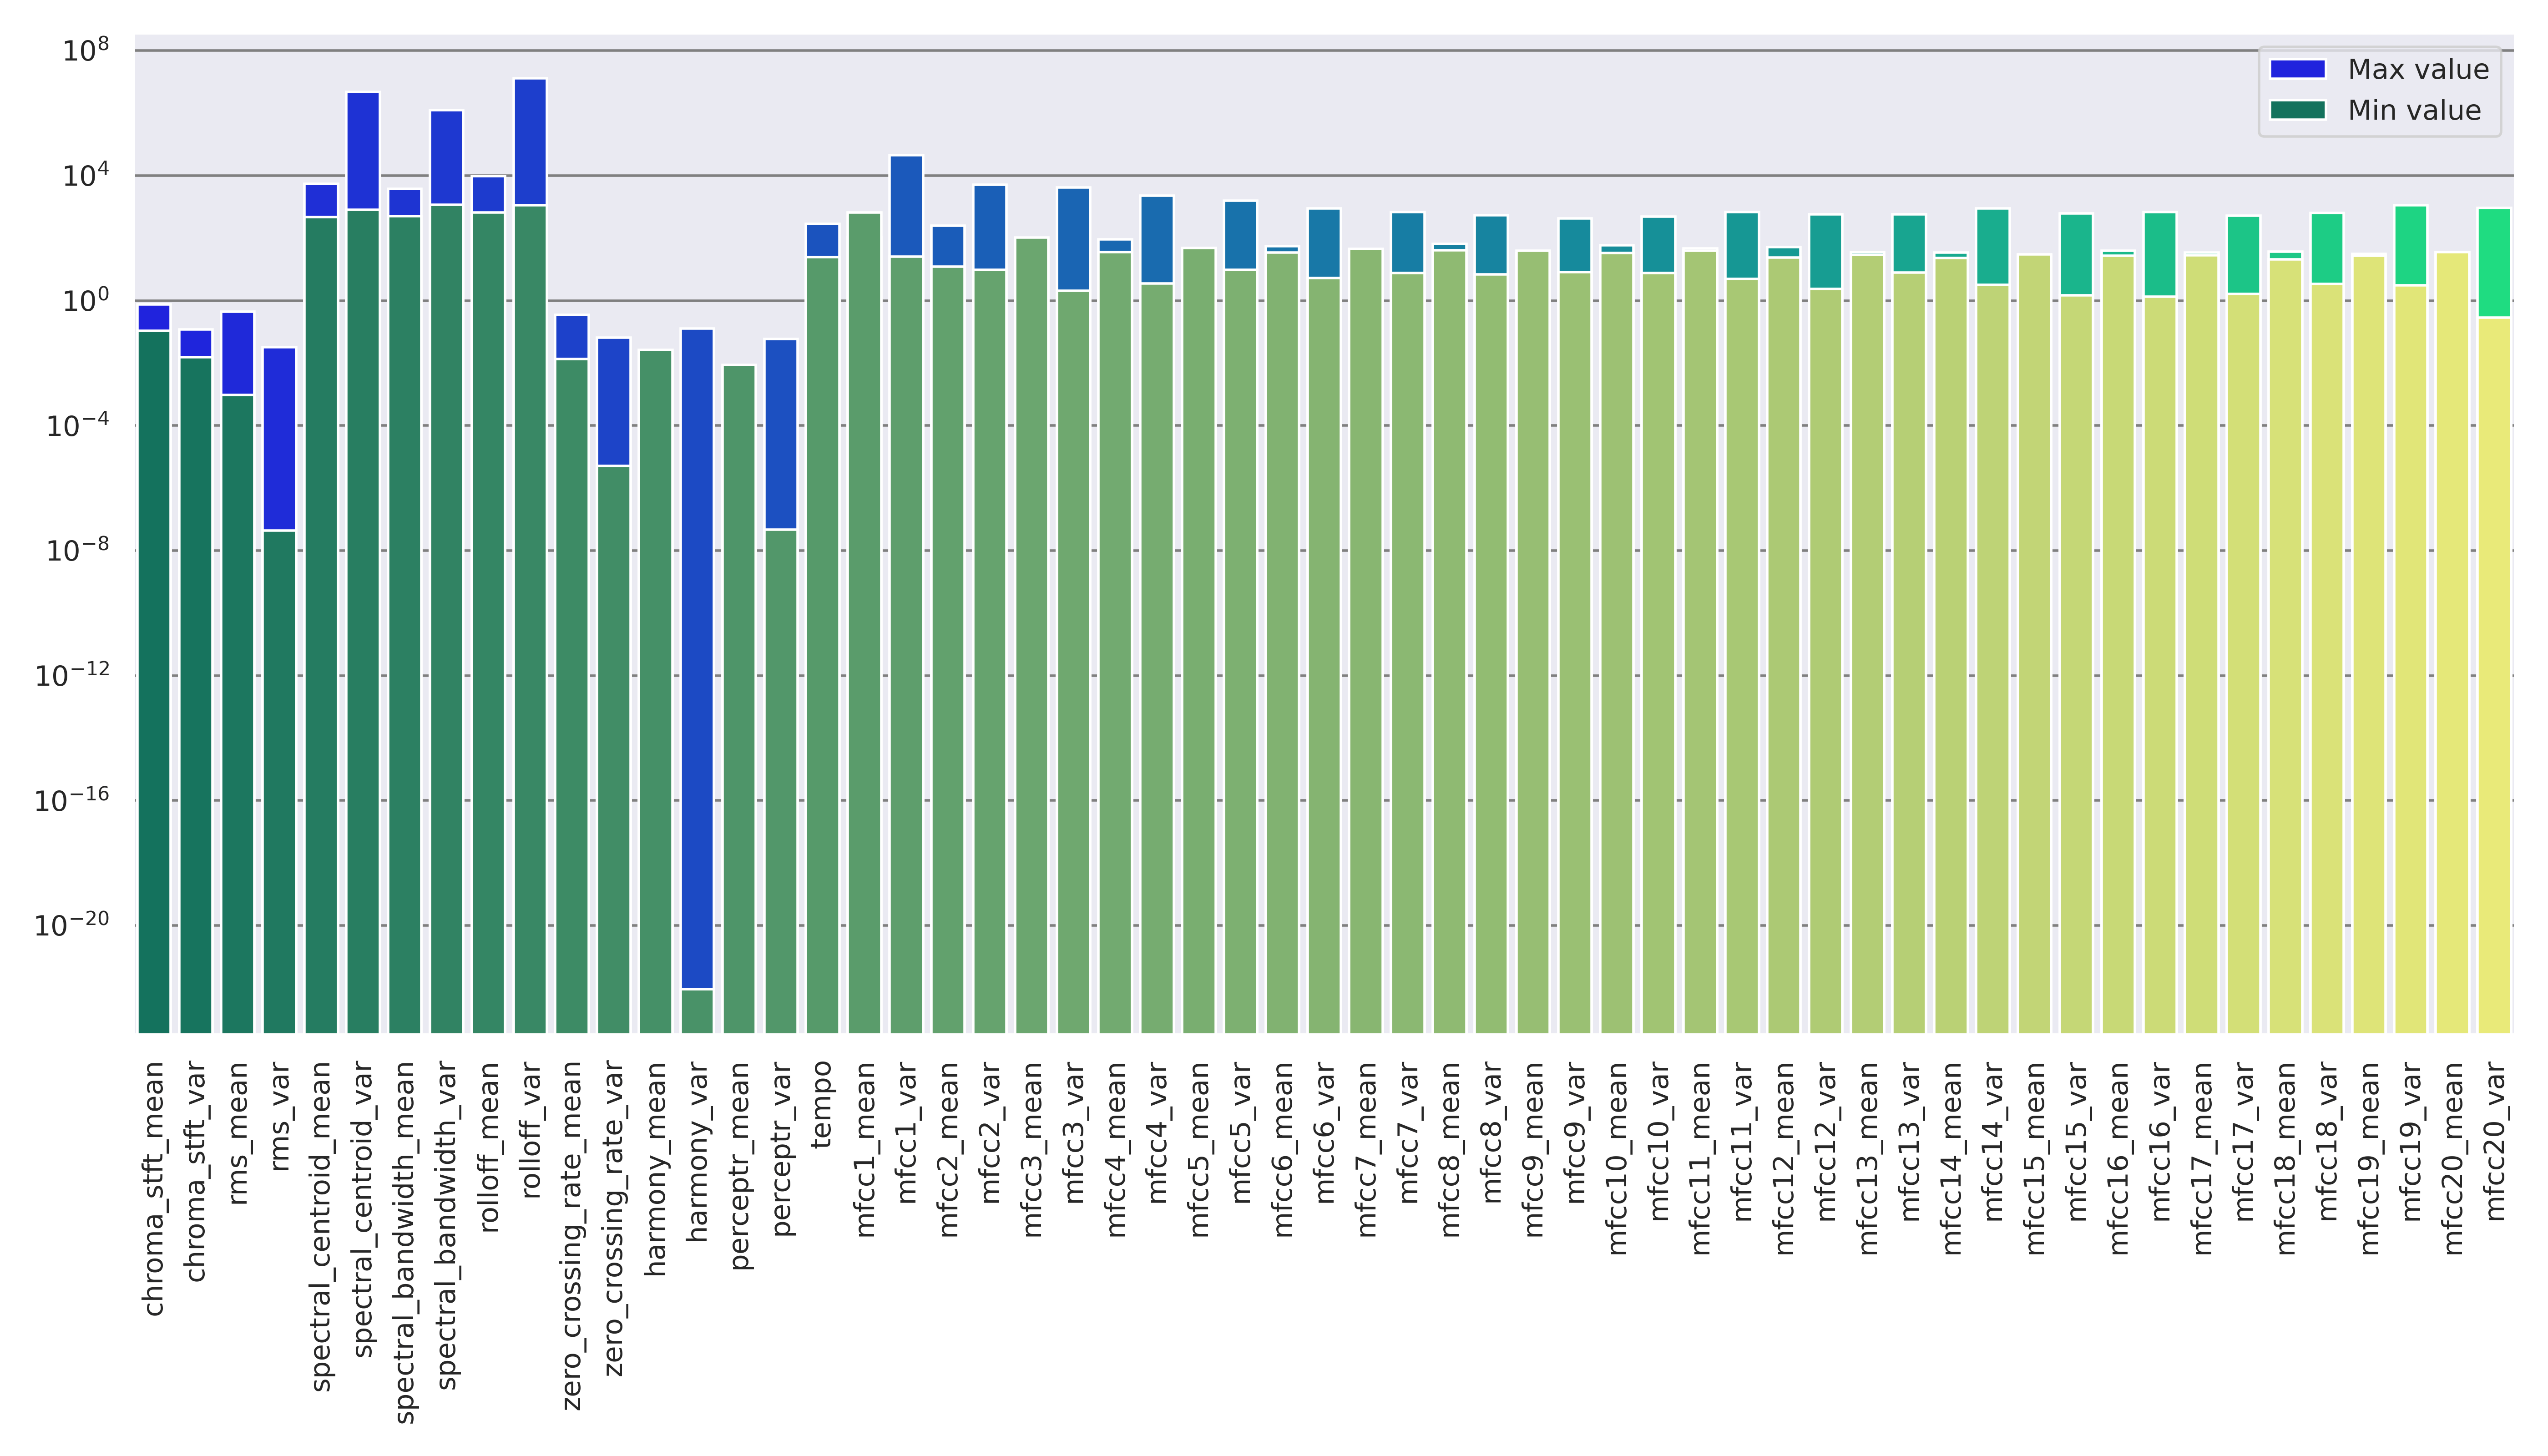
\includegraphics[width=\textwidth]{Figures/datatypes.png}
    \caption{Minimum and maximum values of the features.}
    \label{fig:datatypes}
\end{figure}

It is evident that no variable presents an absolute value that is larger than $10^8$. Therefore, there is no need to use the \textit{float64} data type assigned by \textit{pandas}, we can safely use the \textit{float32} data type without any loss of information. Furthermore, we assigned the data type \textit{category} to the only remaining categorical variable, i.e. the \textit{label}, leading to additional memory saving. 

At the end of this phase, the size in memory of the data set was reduced by a factor of almost 2.

\section{Correlation analysis}
\label{sec:corr}%
The goal of this phase was to find out how the features in the GTZAN data set are related to the target variable. Given the lack of expert knowledge in this field, this analysis is the only way for us to identify which are the most promising features. The correlation is computed through the use of the Predictive Power Score (PPS) \cite{pps}. The PPS is a more powerful metric w.r.t. the linear correlation coefficient since it can also detect non-linear relationships between features. The score ranges from 0 (no predictive power) to 1 (perfect predictive power).

\begin{figure}[H]
    \centering
    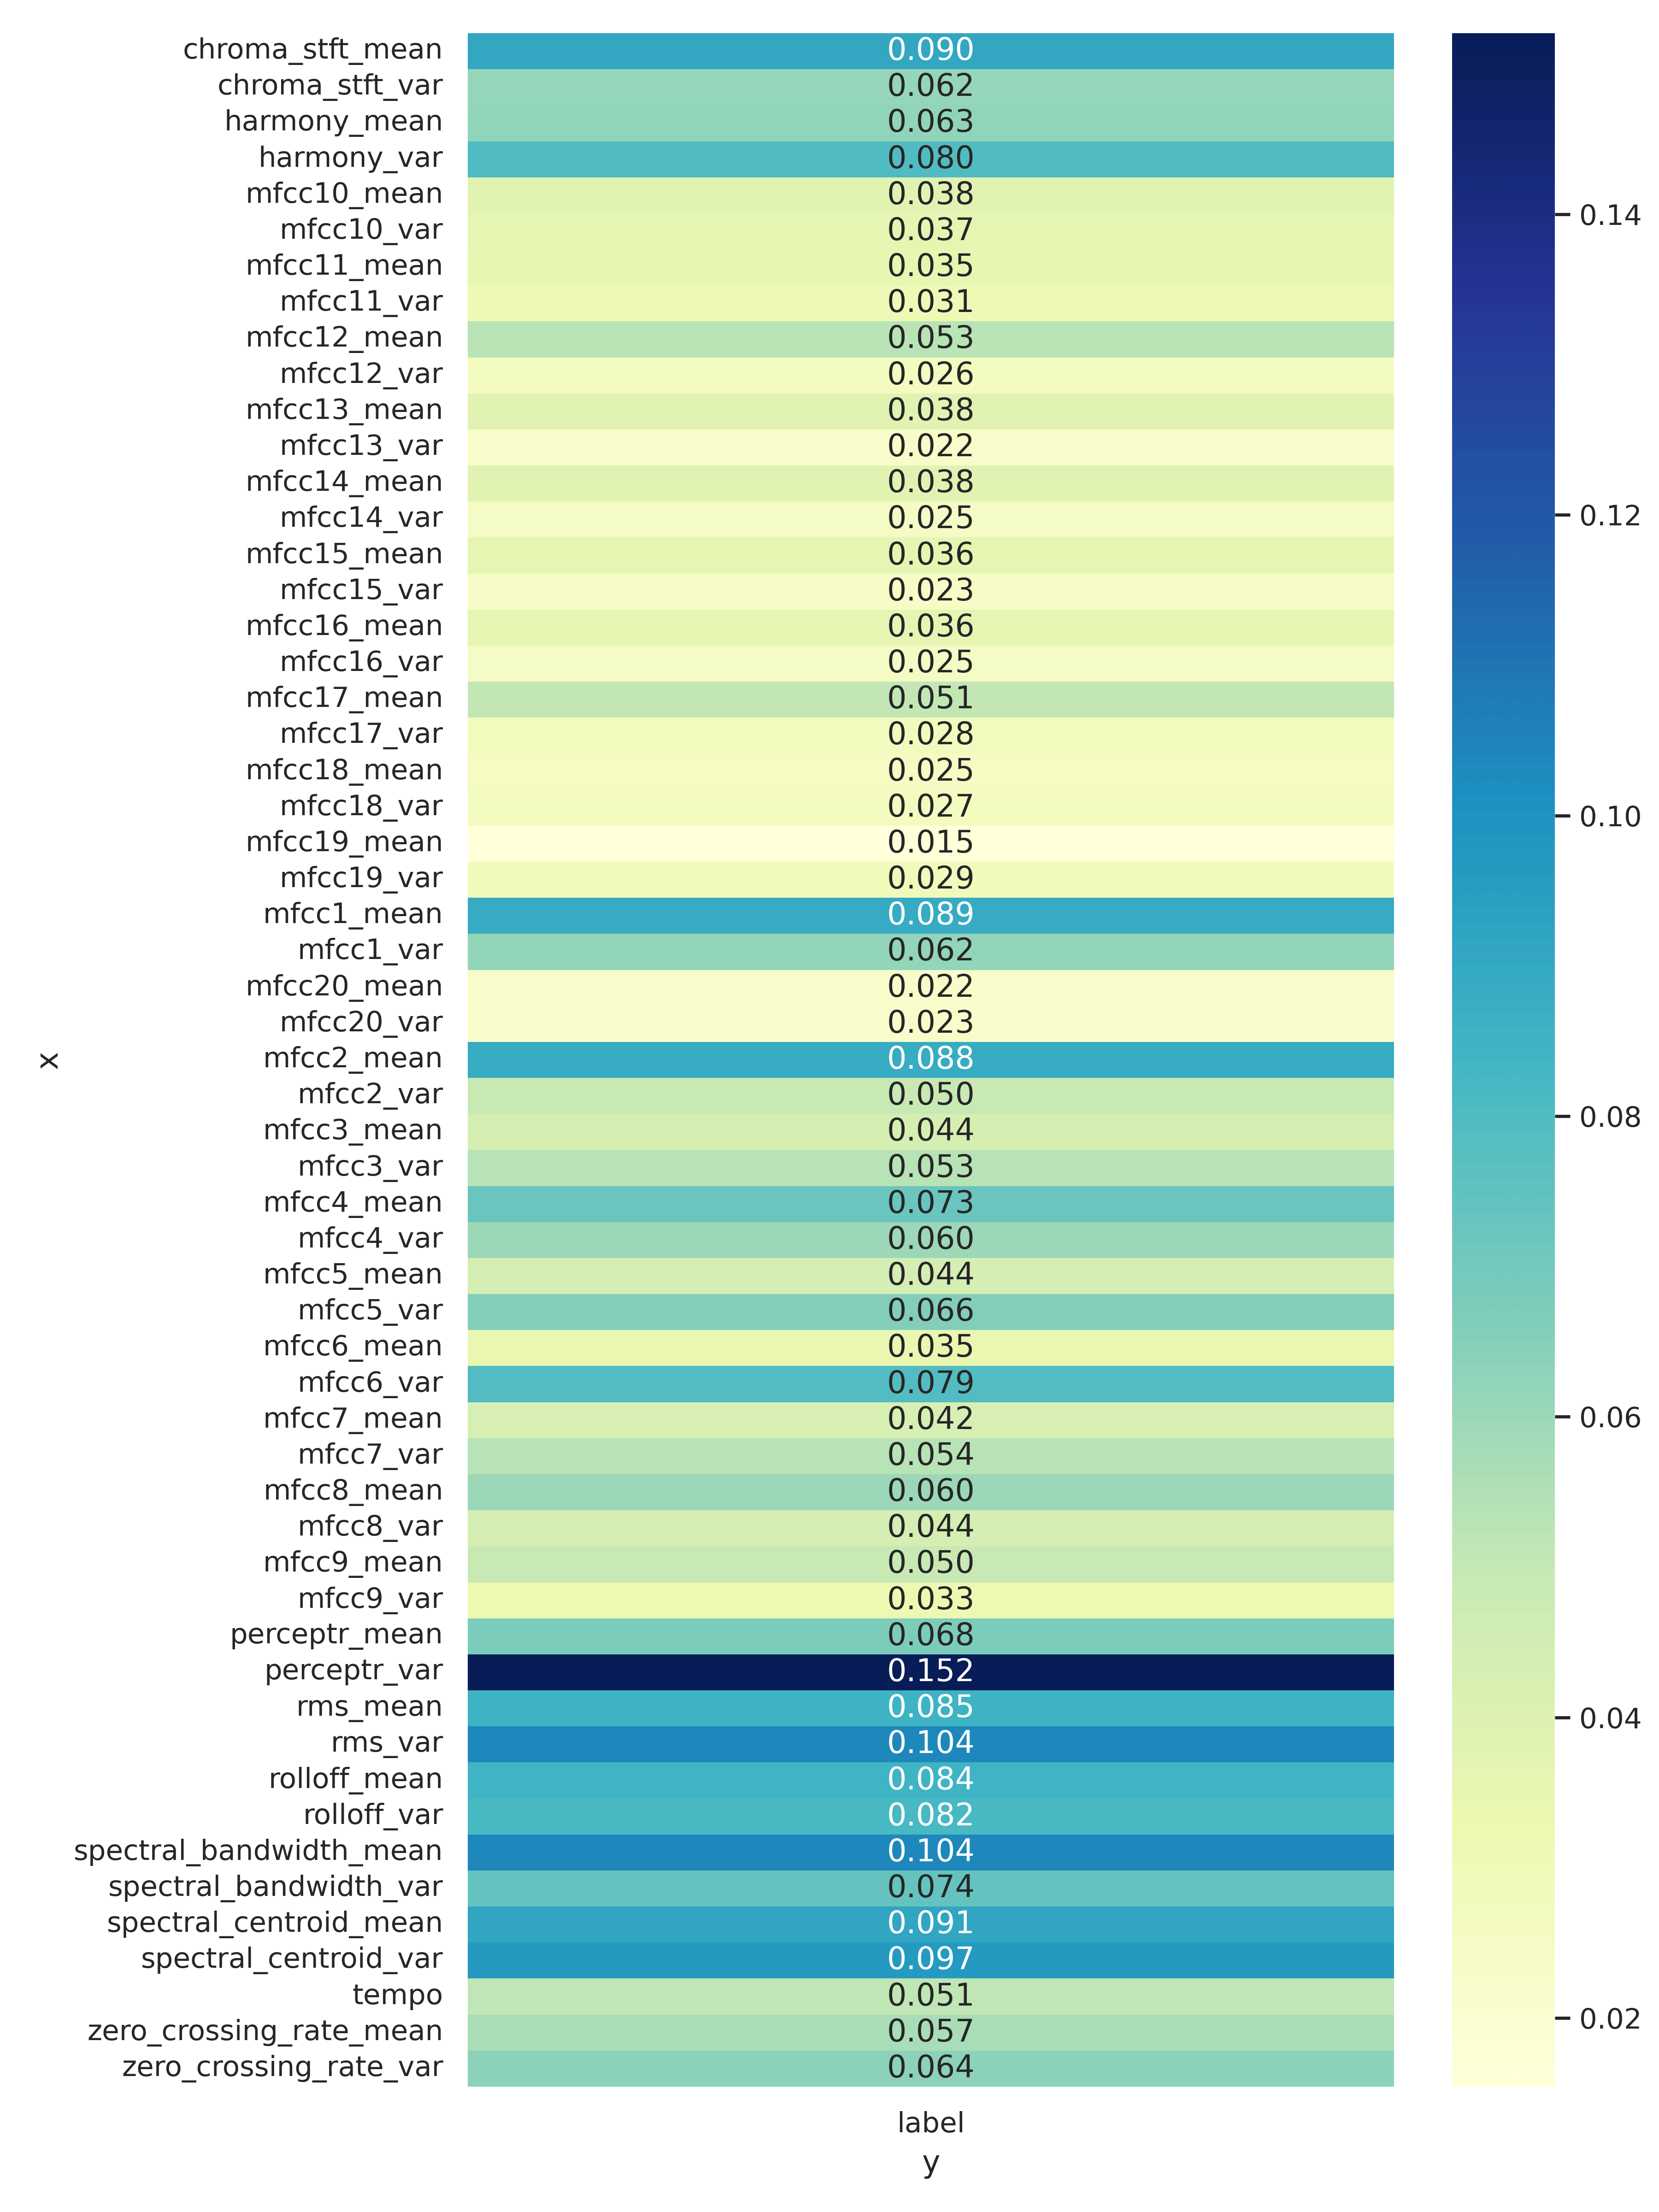
\includegraphics[width=\textwidth]{Figures/corr_all.png}
    \caption{Predictive Power Score w.r.t. the label of all the features.}
    \label{fig:corr_all}
\end{figure}

From the above chart, we can see that many features have a very weak correlation.  \\
We plot below the features with a reasonable level of correlation:

\begin{figure}[H]
    \centering
    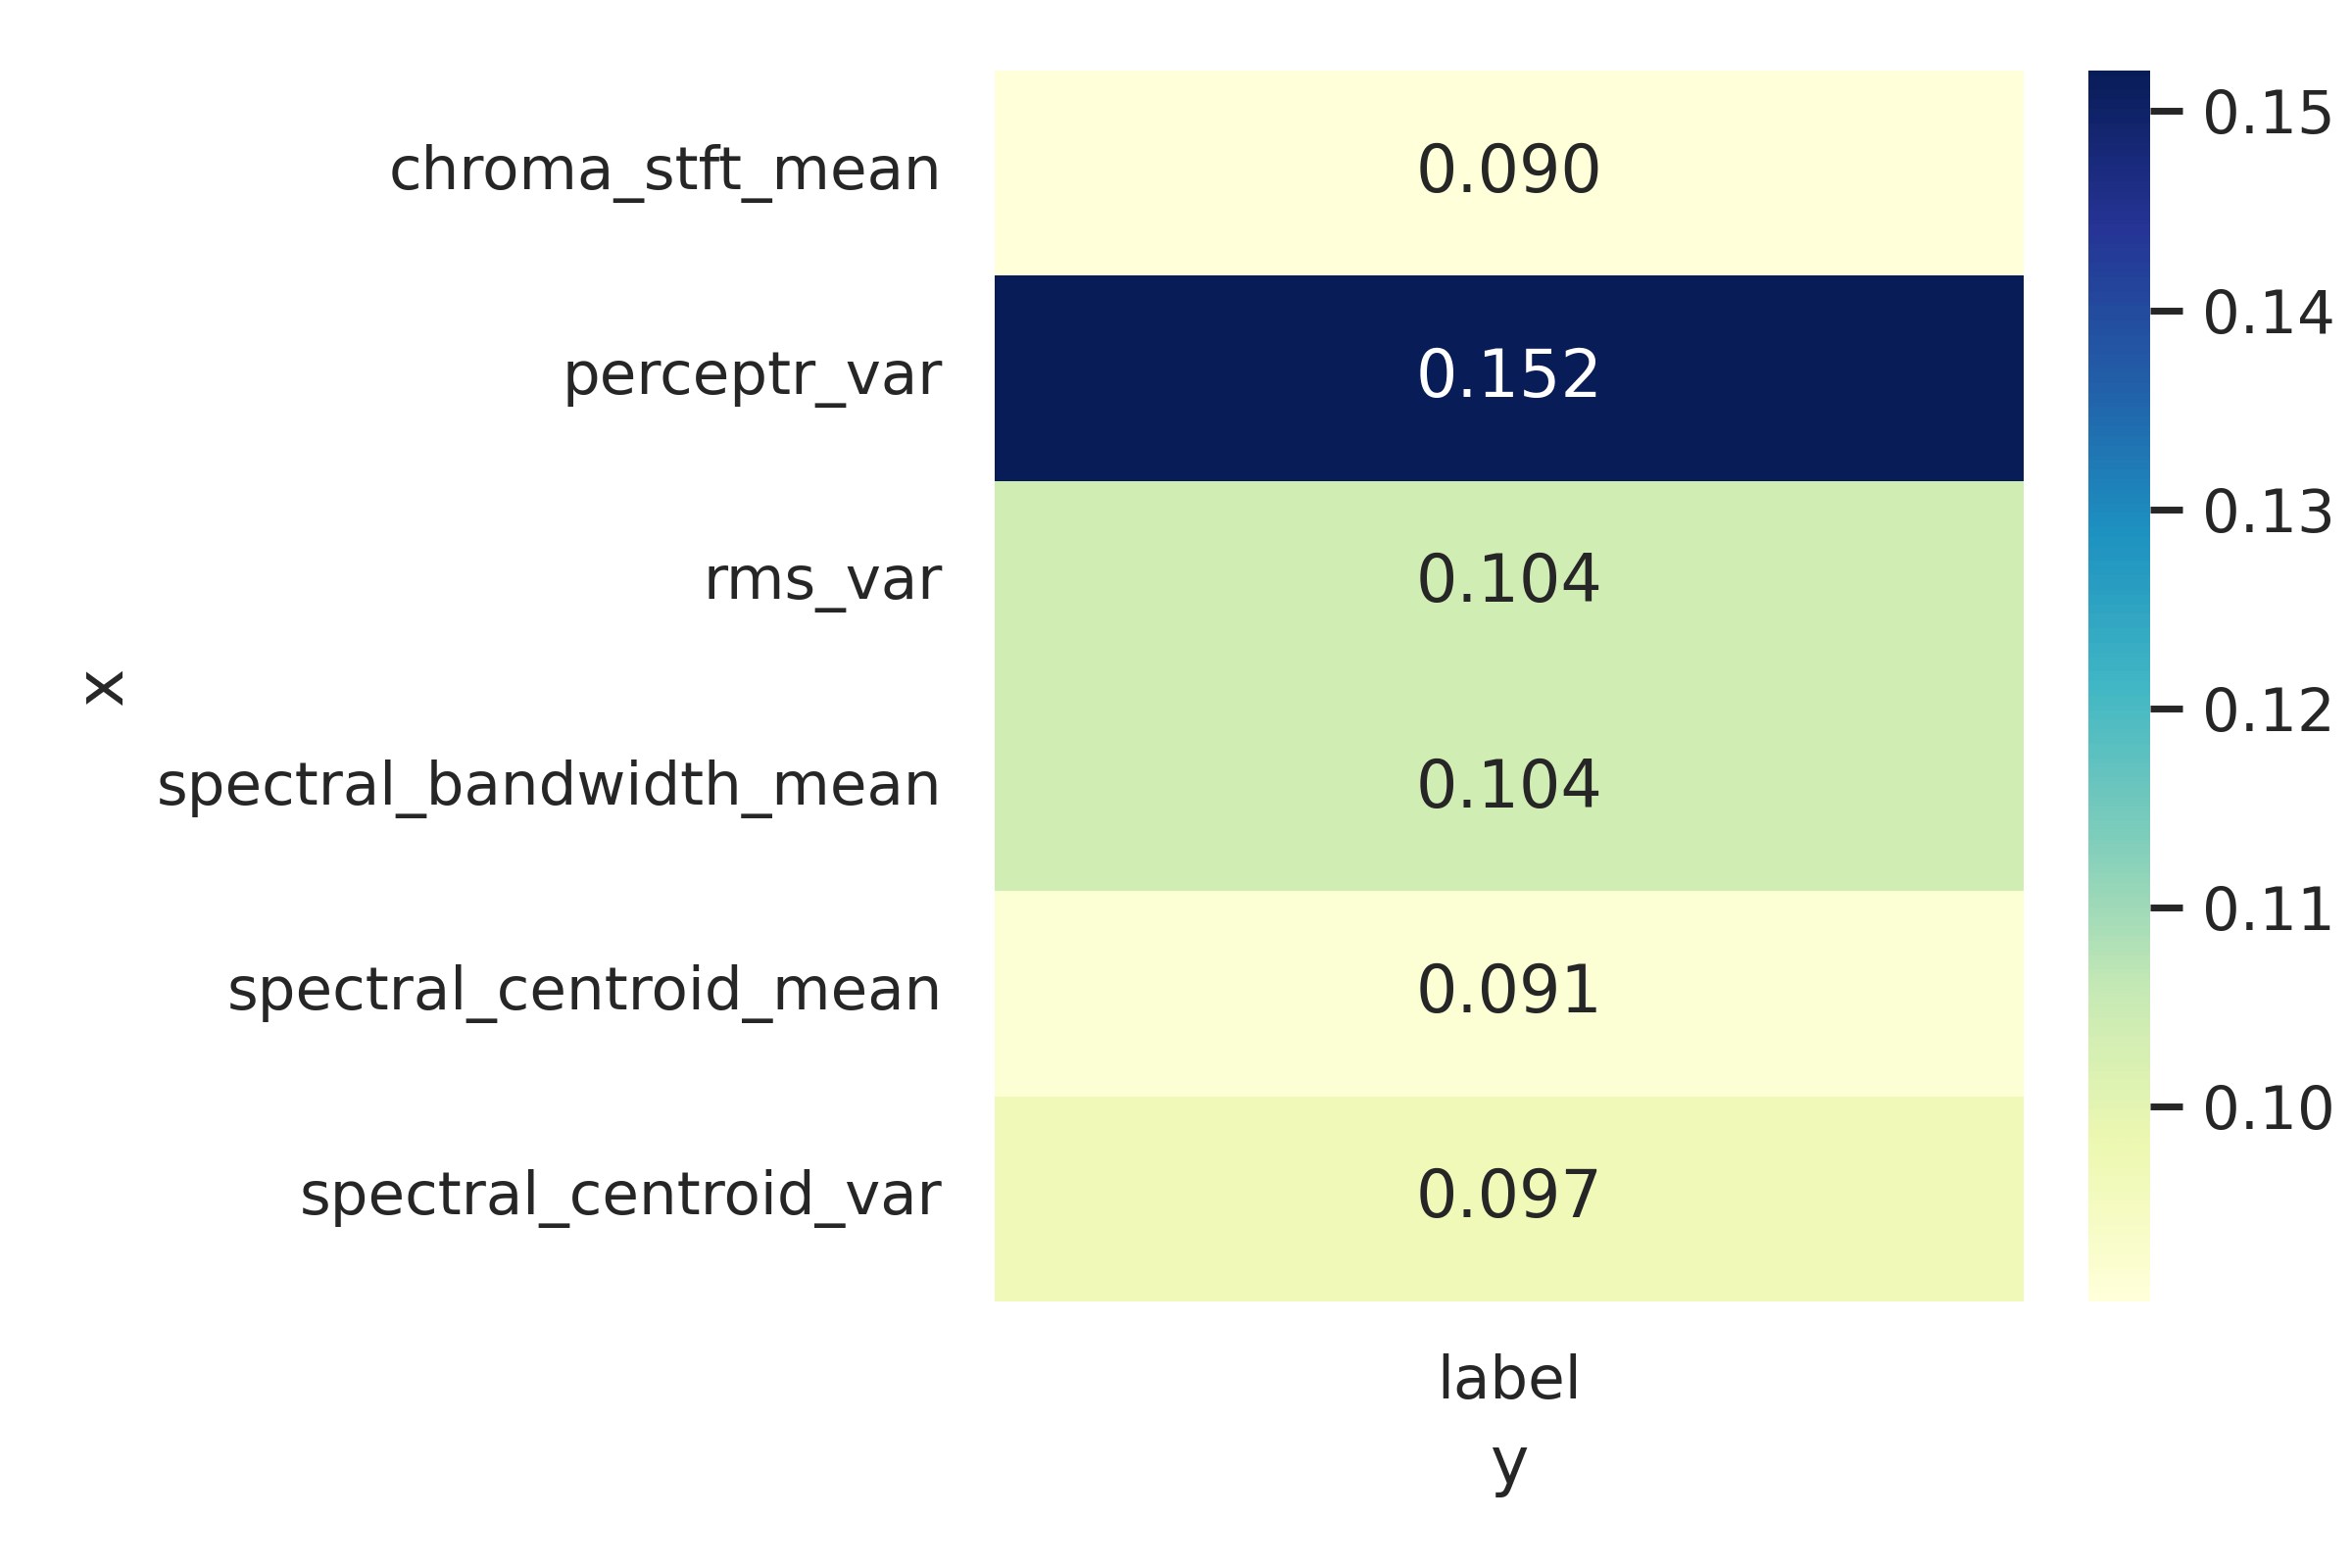
\includegraphics[width=0.7\textwidth]{Figures/corr_high.png}
    \caption{Features with the highest PPS w.r.t. the label.}
    \label{fig:corr_high}
\end{figure}

If we were to perform feature selection, we will certainly keep these features.  \\
However, in this project, we are going to use all the features anyway since the data set is not that large, and since we trust the fact that all the features in the original data set were selected because they were meaningful.

\section{Data visualization}
\label{sec:visualization}%
In order to visualize the data and understand its structure, we will use Principal Component Analysis (PCA), computed through Singular Value Decomposition (SVD). In the following chart, we can see the singular values of the matrix that represents the data set after the PCA was applied.

\begin{figure}[H]
    \centering
    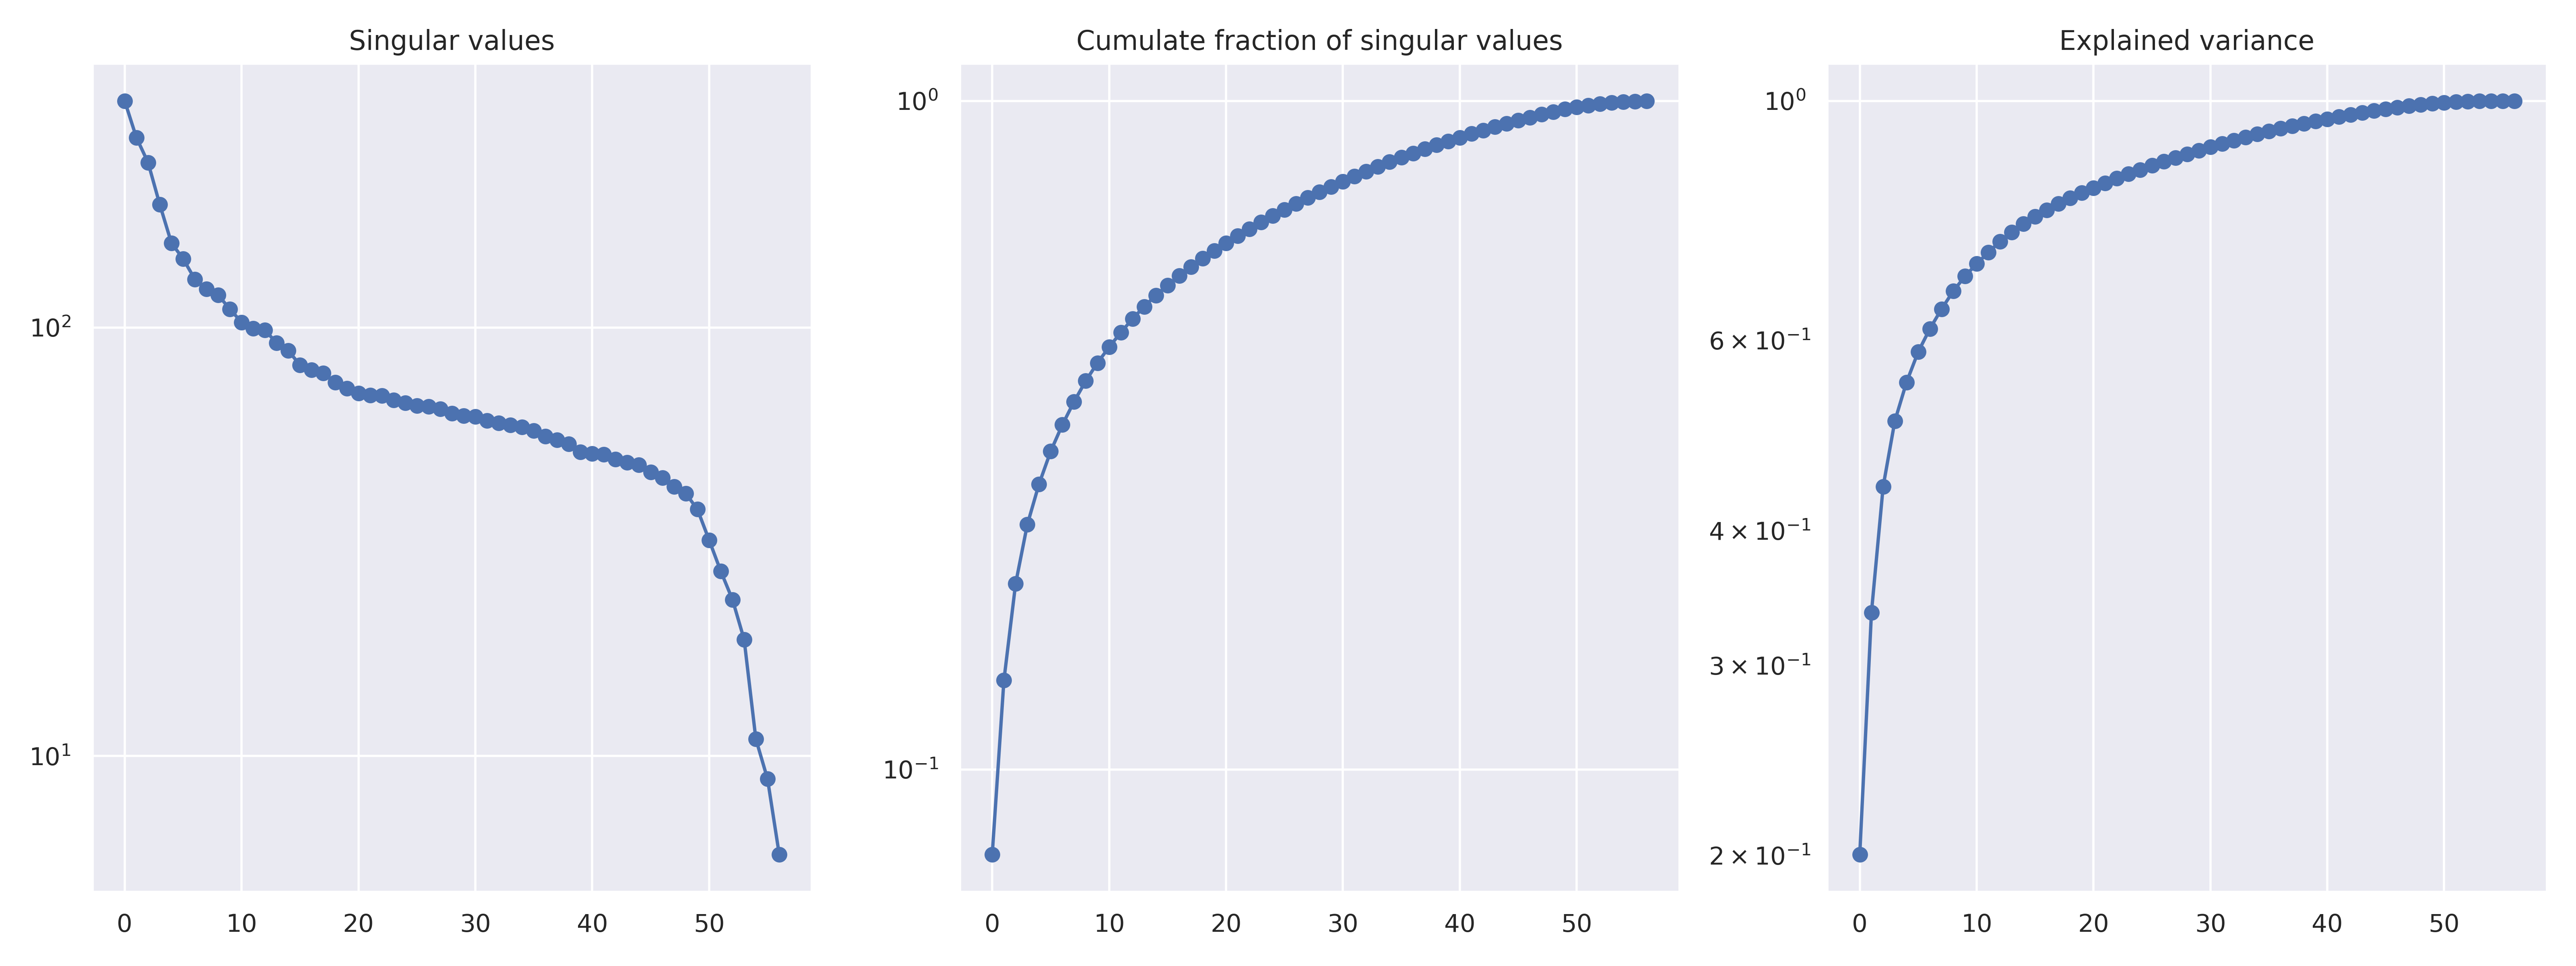
\includegraphics[width=\textwidth]{Figures/singular_values.png}
    \caption{Singular values from PCA and their explained variance.}
    \label{fig:singular_values}
\end{figure}

We could remove some singular values in order to reduce the size of the data leading to a negligible loss of information. However, size is not a concern with this data set and we are not interested in size reduction. 
Instead, we can understand from the explained variance of the singular values that the data we are working with has a complex structure. In fact, we can see that we need to keep a lot of dimensions in order to explain 90\% or more of the variance. The following table contains some significative examples of the amount of variance that we can explain using only a subset of the singular values:

\begin{table}[H]
    \centering 
    \begin{tabular}{|c | c |}
    \hline
    \rowcolor{bluepoli!40} 
     Number of singular values & Explained variance \T\B \\
    \hline \hline
    1 & 20.05\%     \T\B \\
    2 & 33.60\%     \T\B \\
    3 & 43.94\%     \T\B  \\
    4 & 50.54\%     \T\B  \\
    31 & 90.67\%   \T\B  \\
    39 & 95.31\%    \T\B  \\
    57 & 100.00\%  \T\B  \\
    \hline
    \end{tabular}
    \\[10pt]
\end{table}

This suggests that the problem at hand is not easy and that low-complexity models will likely struggle at finding a good decision boundary, at least in the multi-class case. 

We will visualize the data after projecting it onto the principal directions, which we know are the directions that contain the highest variance. 

We can see a scatter plot of the two first principal components of each sample:
\begin{figure}[H]
    \centering
    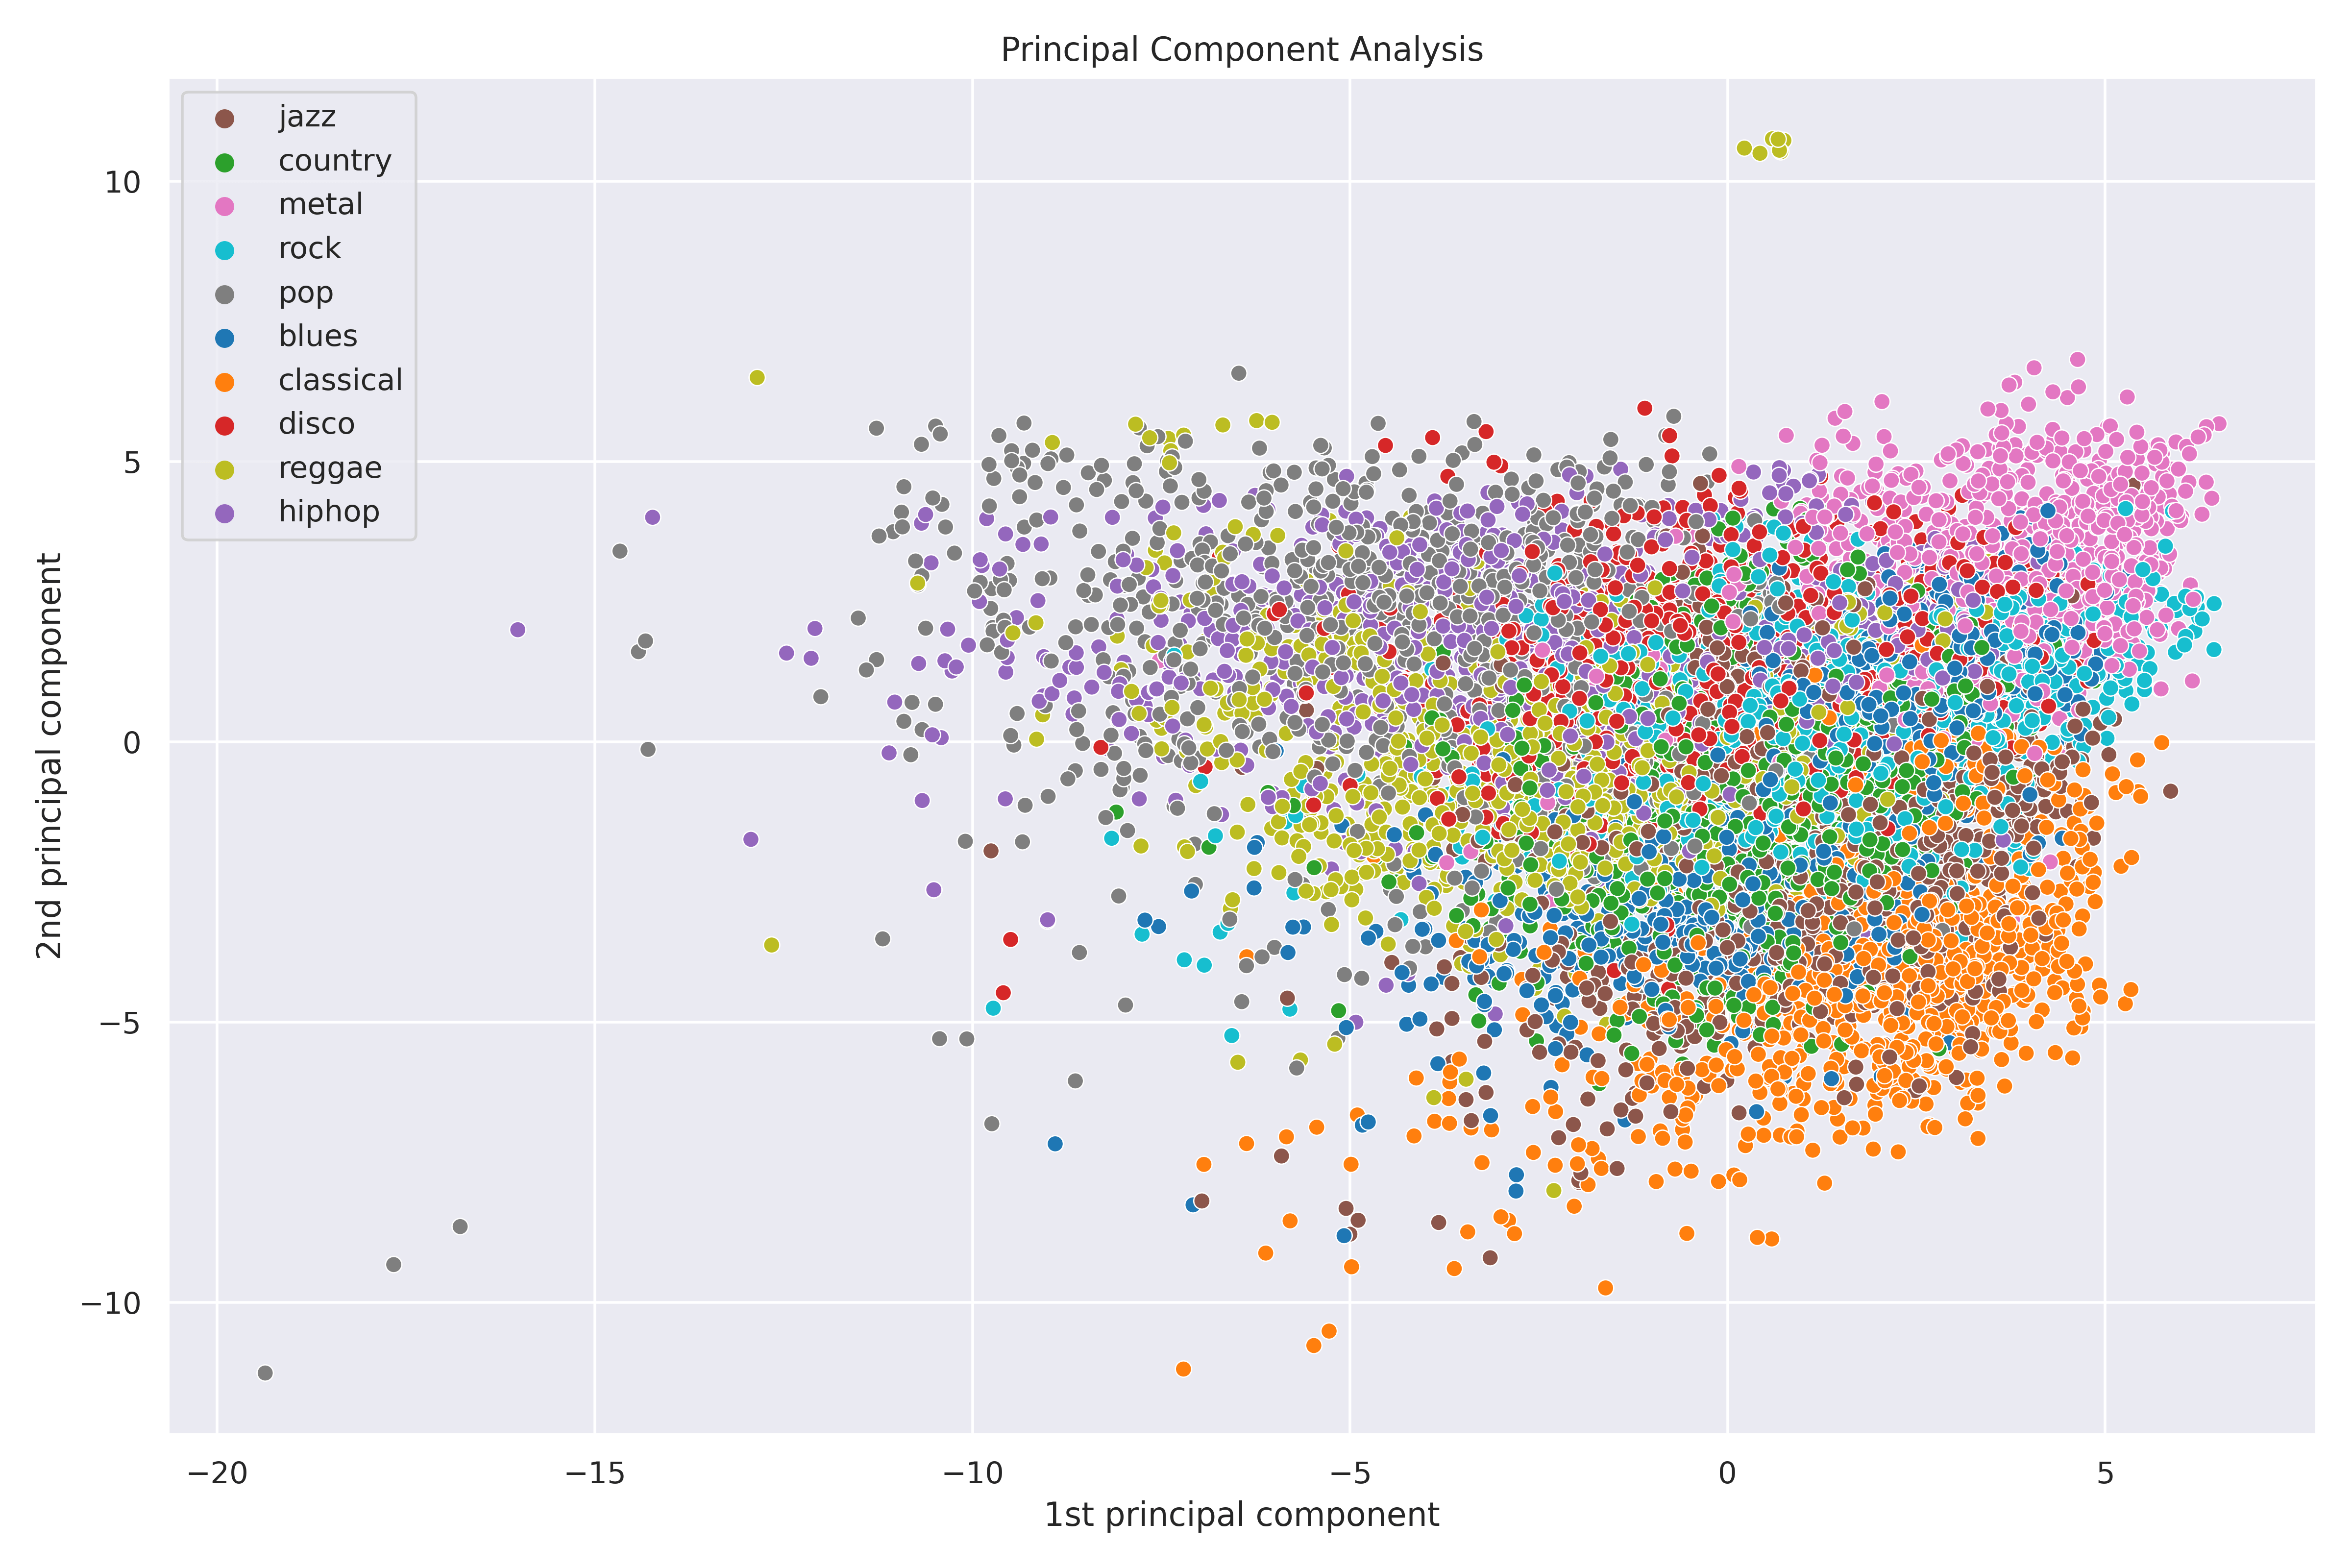
\includegraphics[width=\textwidth]{Figures/pca_2d.png}
    \caption{Scatter plot of the data projected on the two first principal directions.}
    \label{fig:pca2d}
\end{figure}

And a scatter plot of the three first principal components of each sample:
\begin{figure}[H]
    \centering
    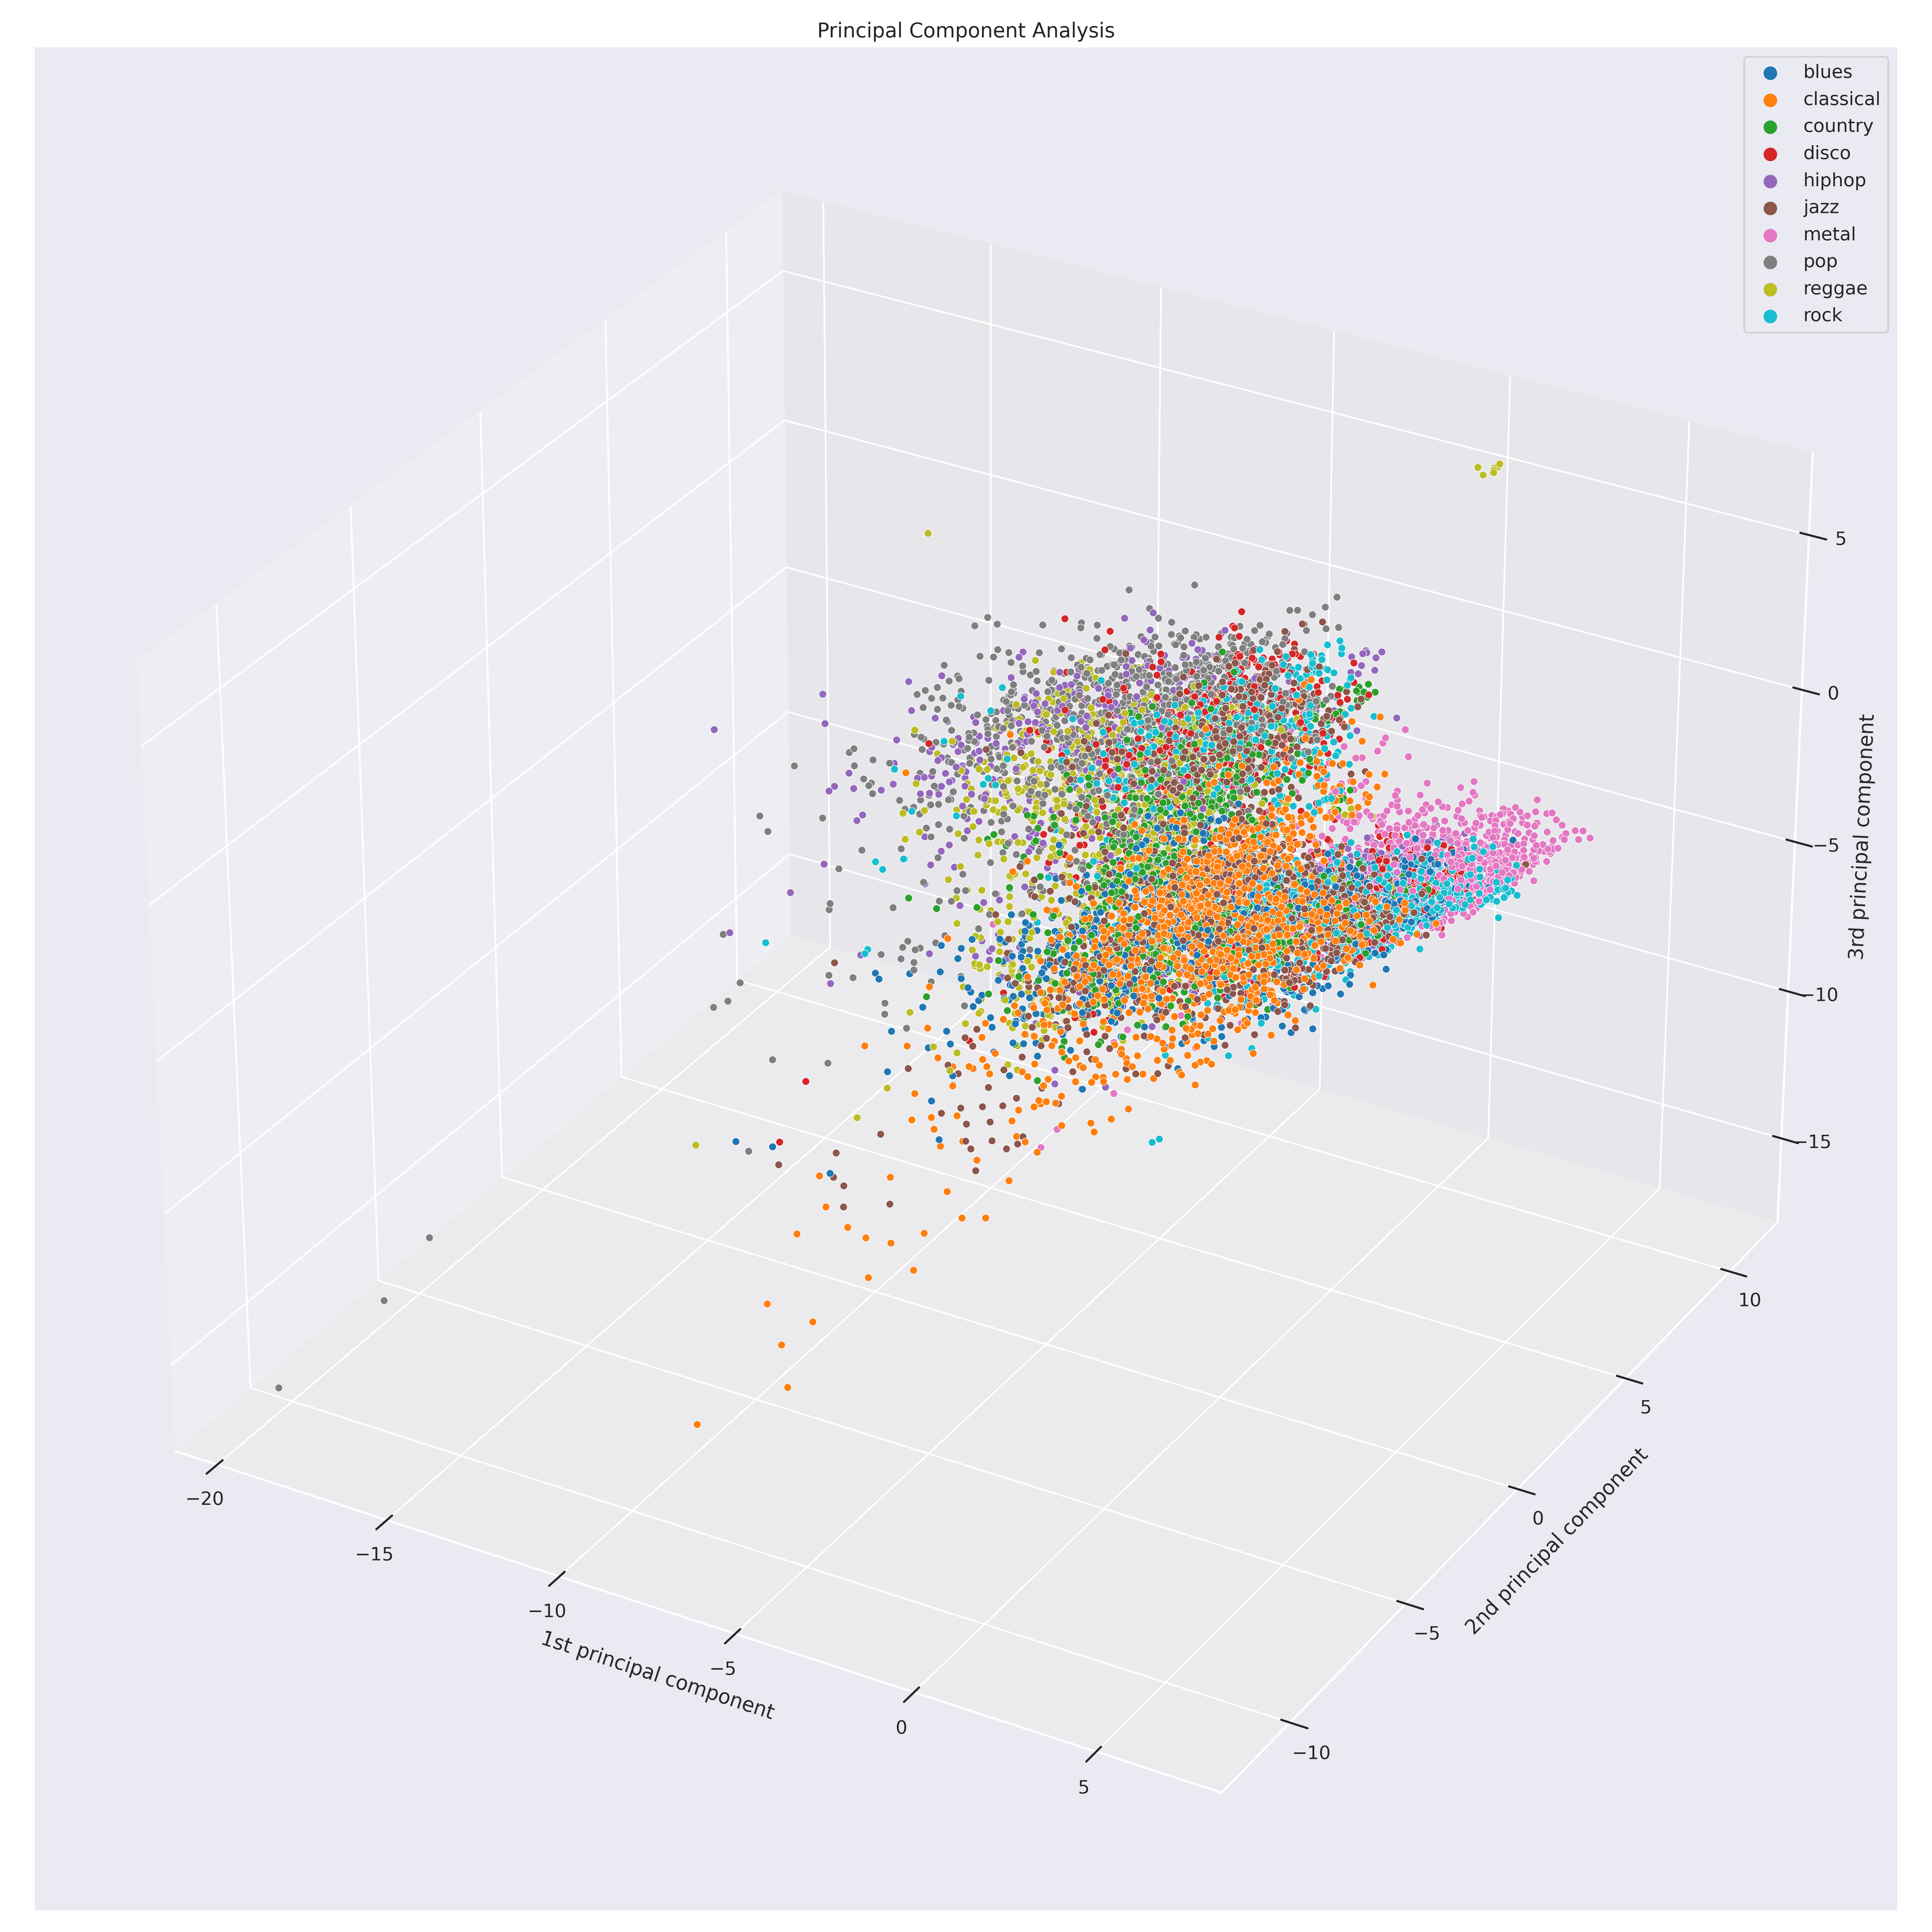
\includegraphics[width=\textwidth]{Figures/pca_3d.png}
    \caption{Scatter plot of the data projected on the three first principal directions.}
    \label{fig:pca3d}
\end{figure}

As expected, it is not easy to visually cluster the data in either of the two plots, even if the situation gets slightly better in the second one. This is expected since as explained earlier we need to use many singular values in order to explain a significant amount of the variance.


\chapter{Machine Learning models}
\label{ch:ml_models}%
In the first part of our analysis, the two classification problems we are considering were tackled using multiple Machine Learning models. The models Naive Bayes (NB) and Voting Feature Intervals (VFI) are the same ones used in the original paper \cite{original-paper}. On the other hand, the CART Decision Trees (DT) and K-Nearest Neighbors (K-NN) models are more modern variants of the ones considered in the paper.

Every model was considered in a separate notebook. Given that those notebooks ended up sharing a large amount of code, many methods were refactored into a separate library file, called \textit{lib.py}, which was then imported into the other notebooks just like a regular library. This file contains many functions useful to perform pre-processing, normalization, label encoding, class balancing and plotting.


\section{Naive Bayes}
\label{sec:nb}%
Naive Bayes methods are a set of supervised learning algorithms based on Bayes’ theorem, with the additional “naive” assumption of conditional independence between every pair of features.

In spite of this over-simplified assumption, Naive Bayes classifiers behave quite well in real-world situations. They require a small amount of training data to estimate the necessary parameters and are known to be extremely fast compared to more sophisticated methods.

On the other hand, although Naive Bayes is known to be a decent classifier, it is also known to be a bad estimator, meaning that the probability outputs that it returns should not be taken too seriously.

In particular, in our analysis, we used the Gaussian Naive Bayes algorithm, which assumes the likelihood of the features to be Gaussian. The code is provided by the library \textit{scikit-learn} \cite{scikit-learn}. 
Every step of this analysis is reported in the notebook \textit{Naive\_Bayes.ipynb}.

Naive Bayes can work with a categorical target variable, therefore it was enough to normalize the data through standardization in order to fit the model. 

In the following charts, we can see the accuracy of the multi-class classifier and of the binary classifiers with different sizes of the train-validation split and with a different number of folds for the K-fold cross-validation.

\begin{figure}[H]
    \centering
    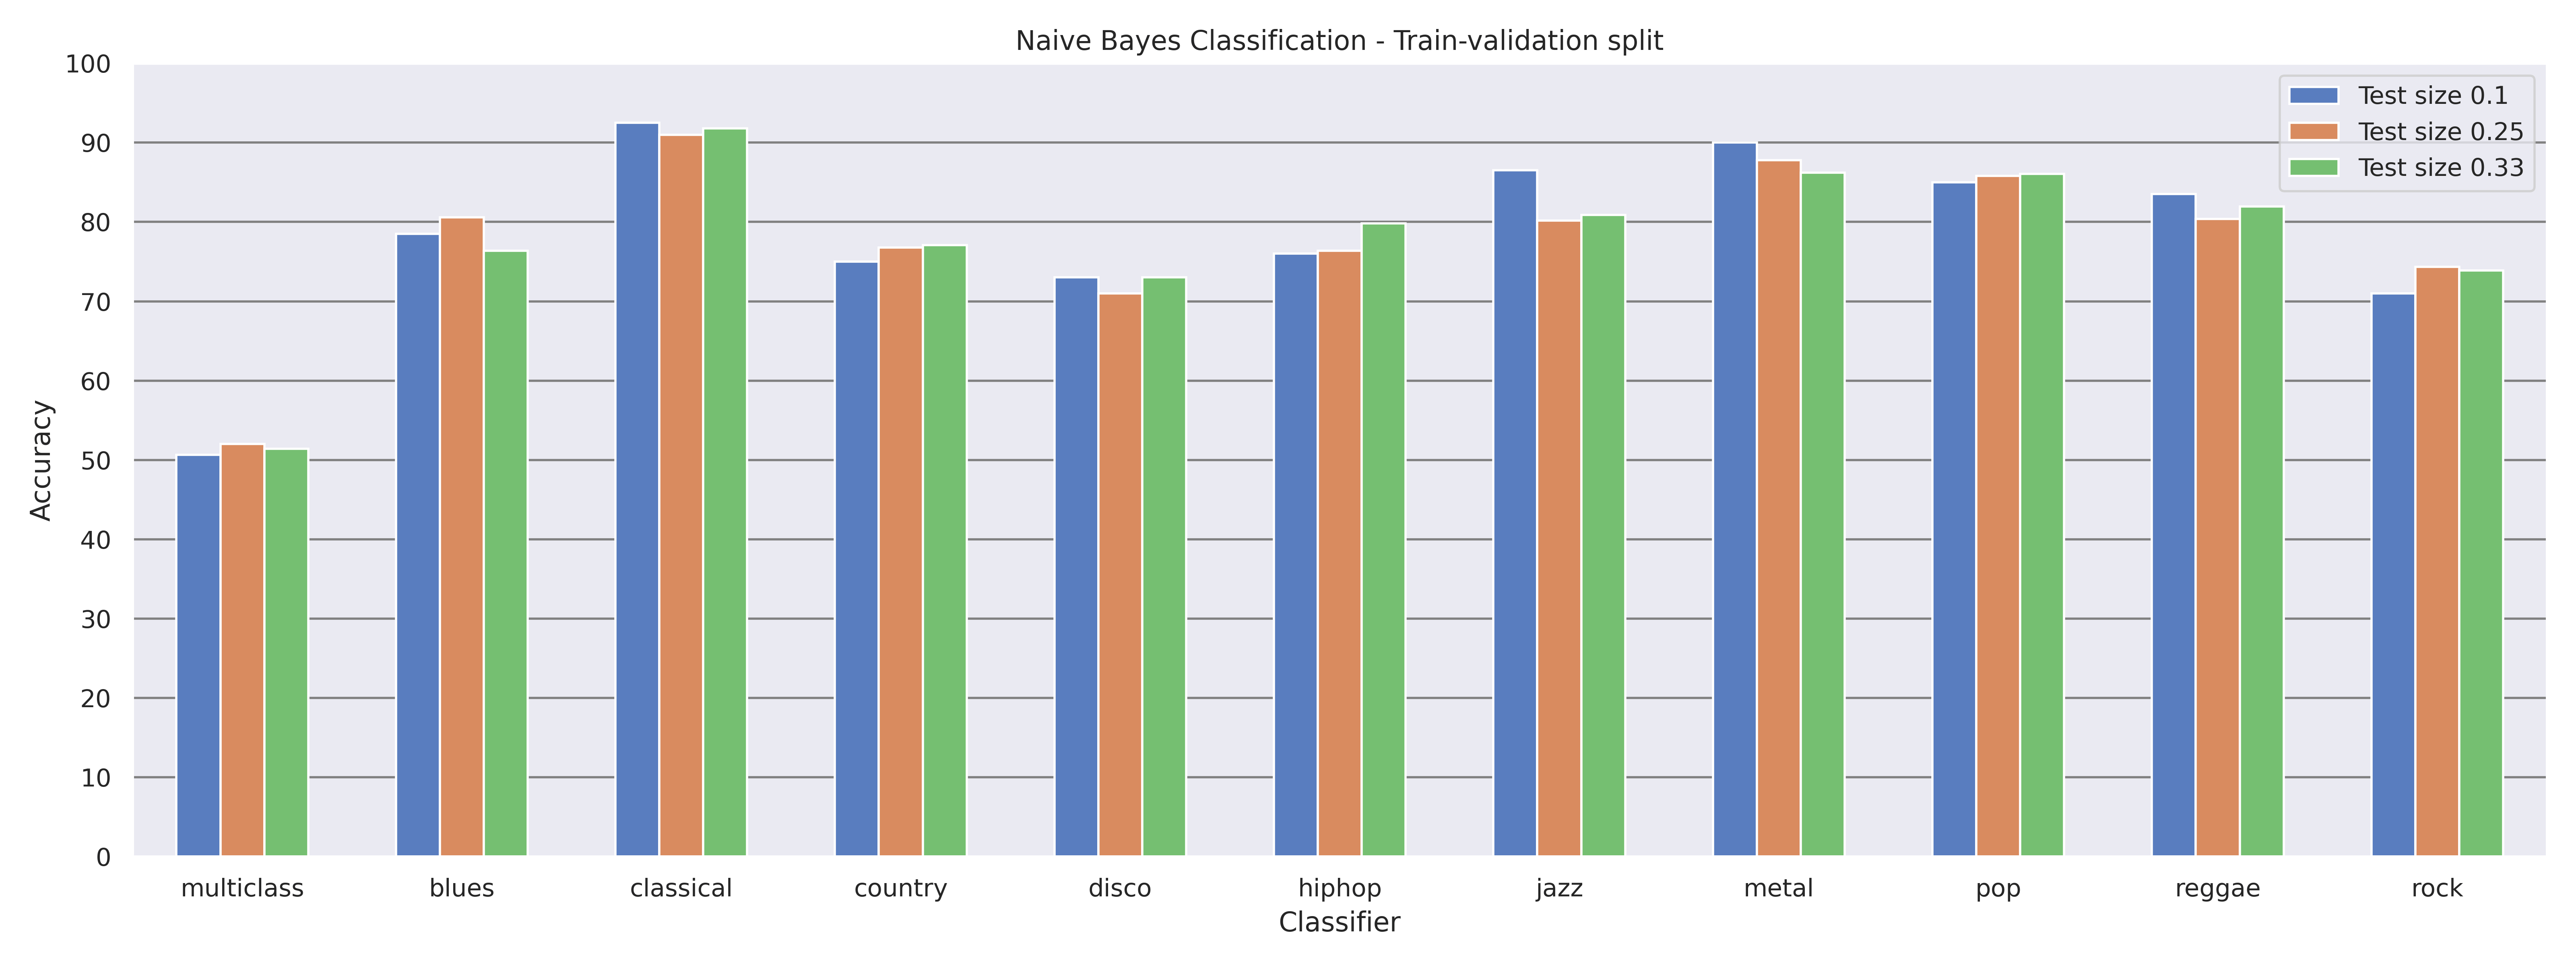
\includegraphics[width=\textwidth]{Figures/nb_s.png}
    \caption{Accuracy of the NB classifier with the train-validation split.}
    \label{fig:nbs}
\end{figure}

\begin{figure}[H]
    \centering
    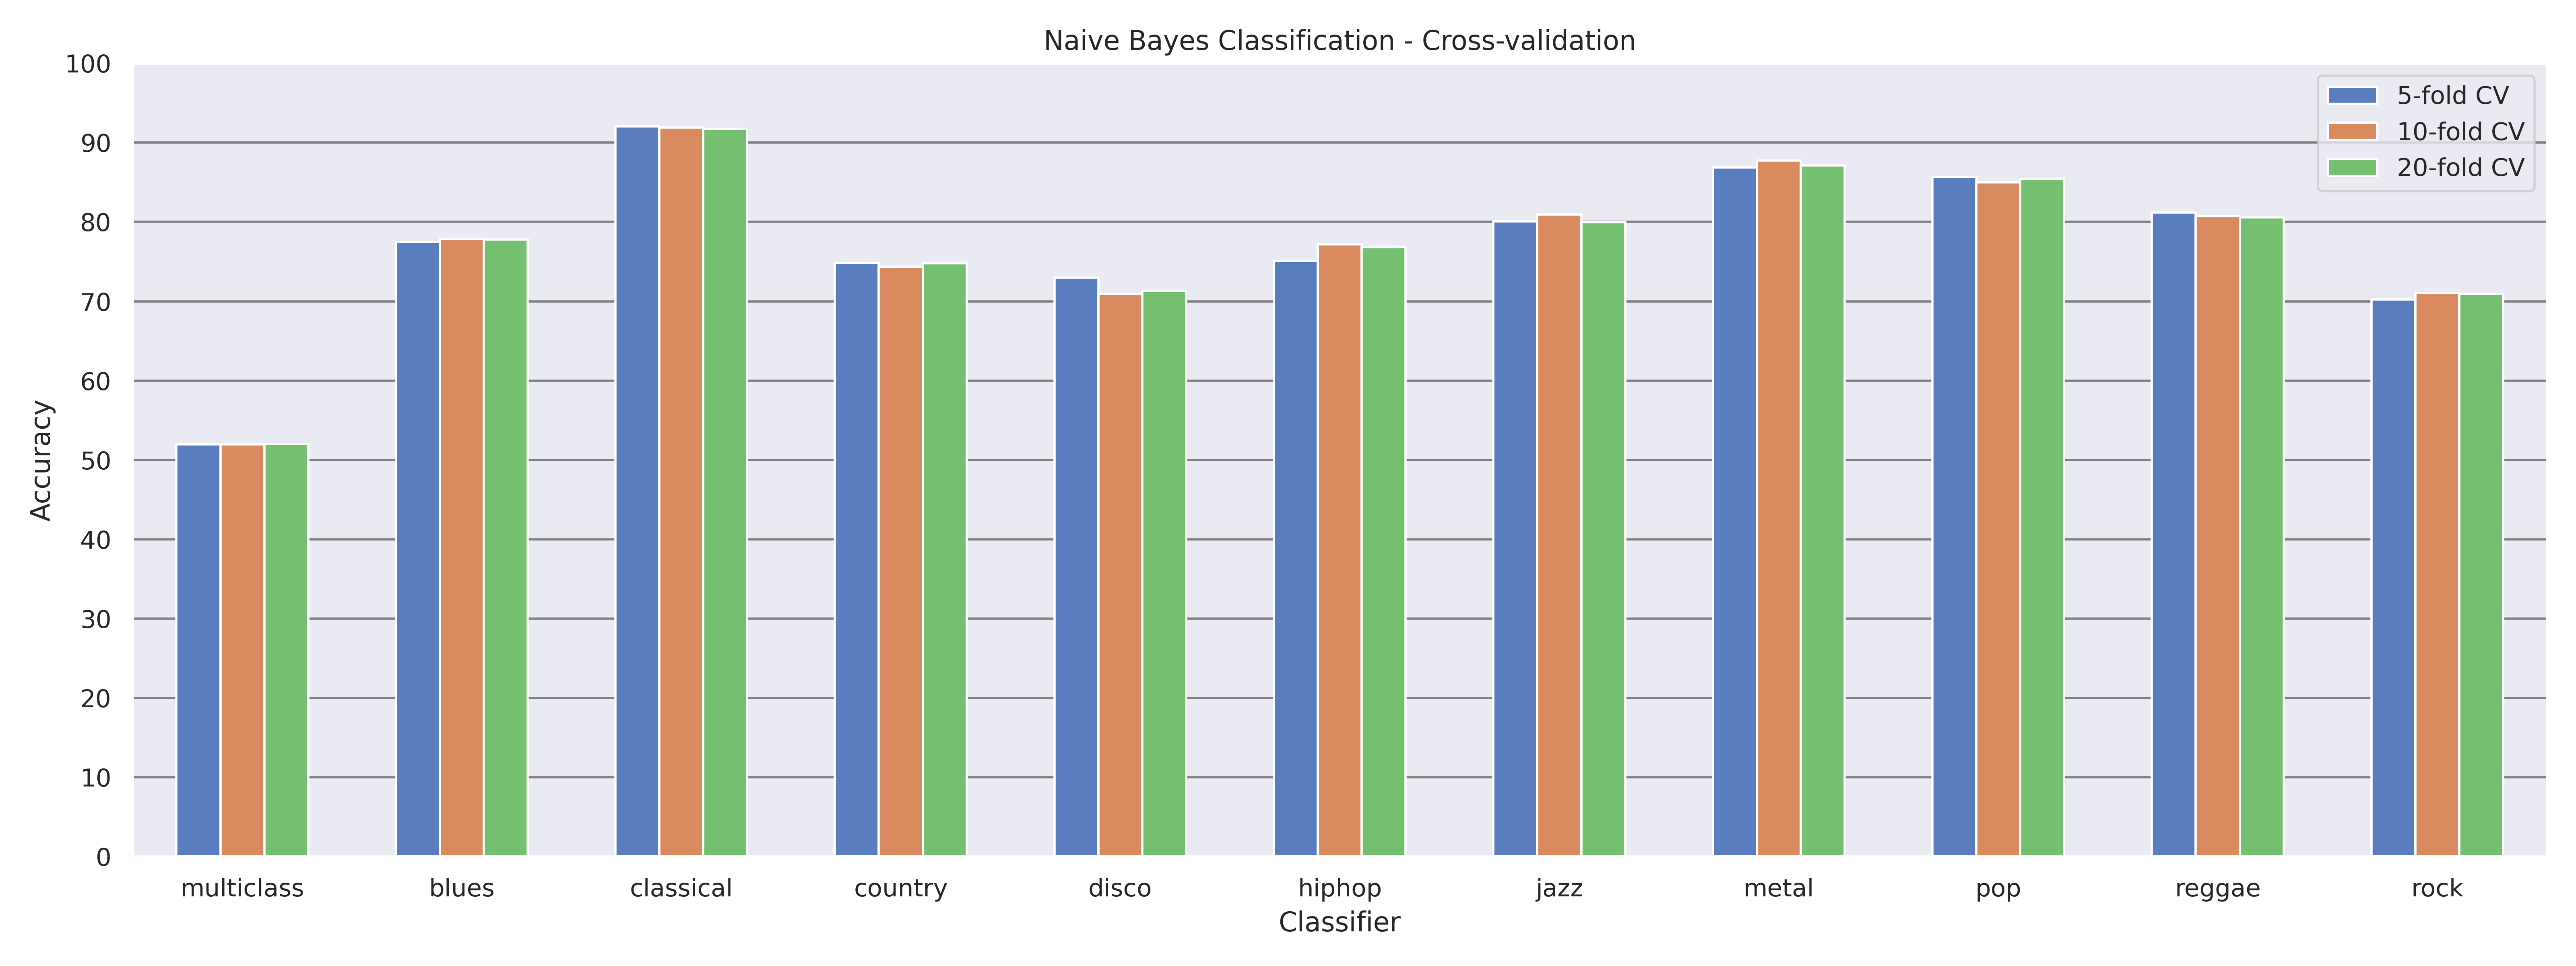
\includegraphics[width=\textwidth]{Figures/nb_d.png}
    \caption{Accuracy of the NB classifier with K-fold cross-validation.}
    \label{fig:nbd}
\end{figure}

We can see that the accuracy, in particular in the multi-class case, is far from good. 
This is expected since, as stated in the EDA, the multi-class classification problem is not easy, and a very simple model like Naive Bayes is not able to handle well this complexity.

The following is the confusion matrix of the multi-class Naive Bayes classifier.

\begin{figure}[H]
    \centering
    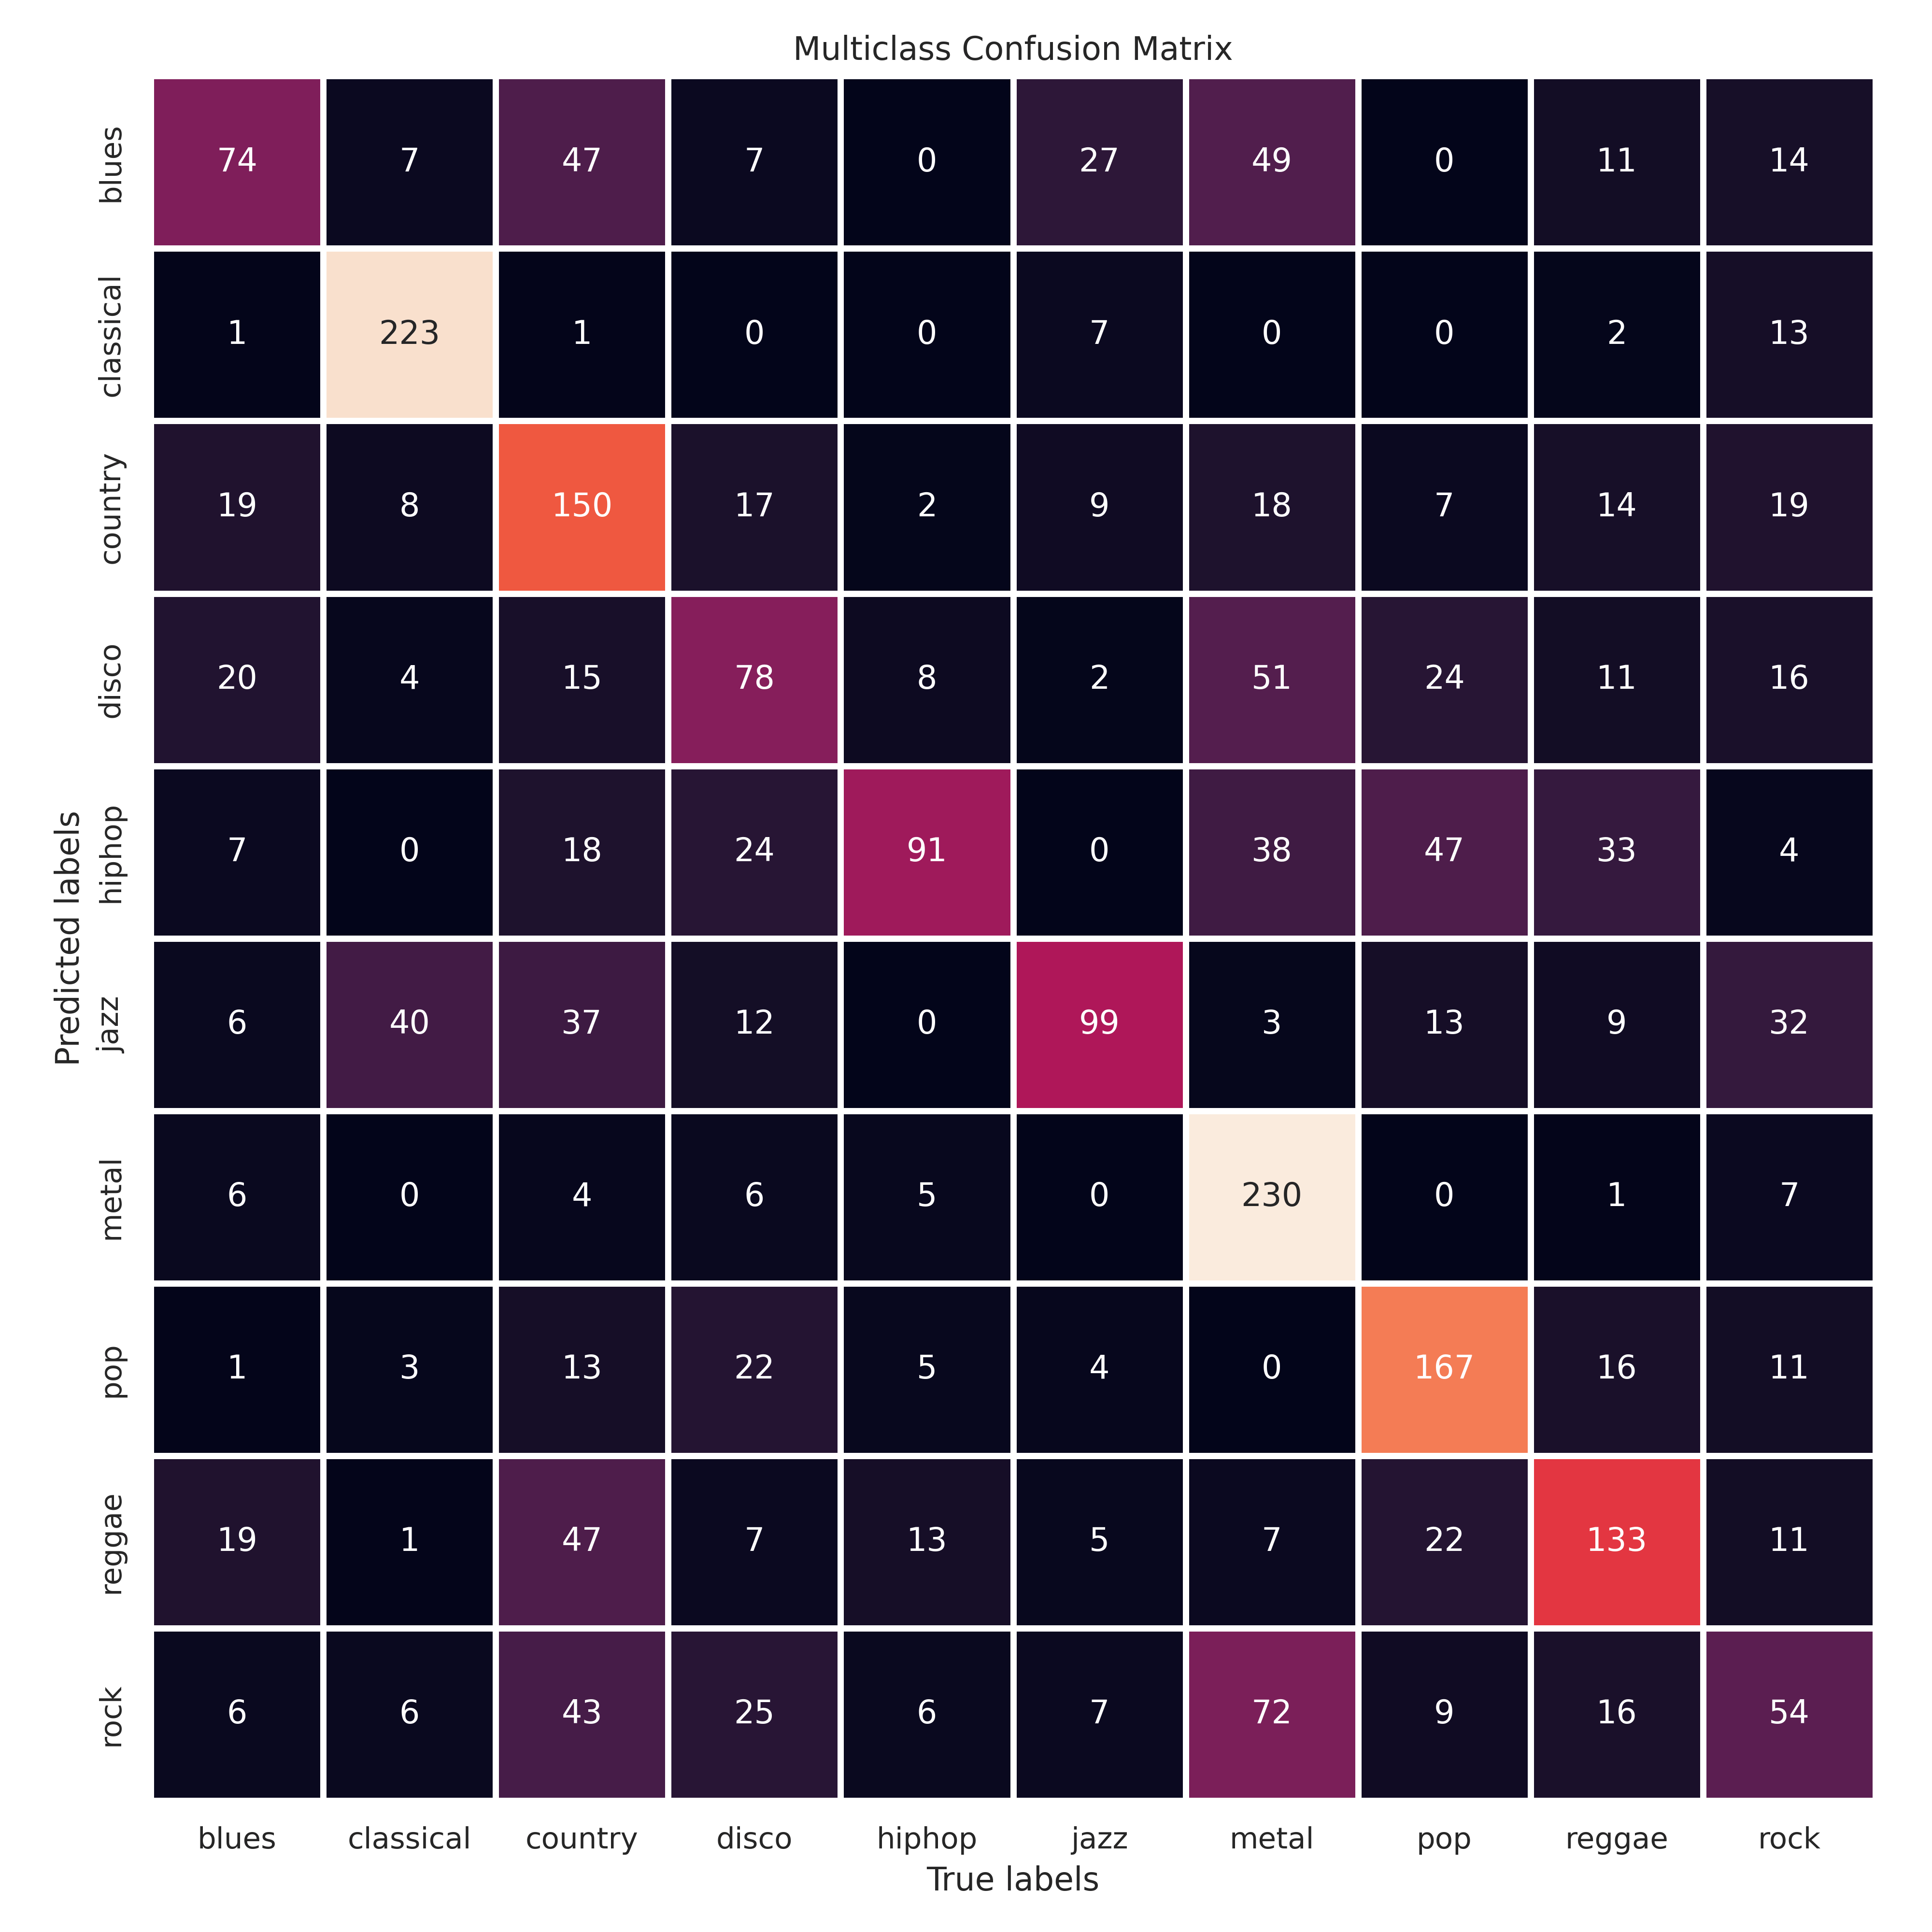
\includegraphics[width=0.7\textwidth]{Figures/nb_m.png}
    \caption{Confusion matrix of the multi-class NB classifier.}
    \label{fig:nbc}
\end{figure}

\pagebreak


\section{Voting Feature Intervals}
\label{sec:vfi}%
Voting Feature Intervals (VFI) is a deterministic supervised classification model similar to Naive Bayes. VFI constructs intervals around each class for each feature. Class counts are recorded for each interval on each feature and the classification is performed using a voting scheme.

The code is provided by the \textit{vfi} Python library, which is maintained in a GitHub repository \cite{vfi}.
Every step of this analysis is reported in the notebook \textit{VFI.ipynb}.

VFI can work with a categorical target variable, therefore it was enough to normalize the data through standardization in order to fit the model. 

In the following charts, we can see the accuracy of the multi-class classifier and of the binary classifiers with different sizes of the train-validation split and with a different number of folds for the K-fold cross-validation.

\begin{figure}[H]
    \centering
    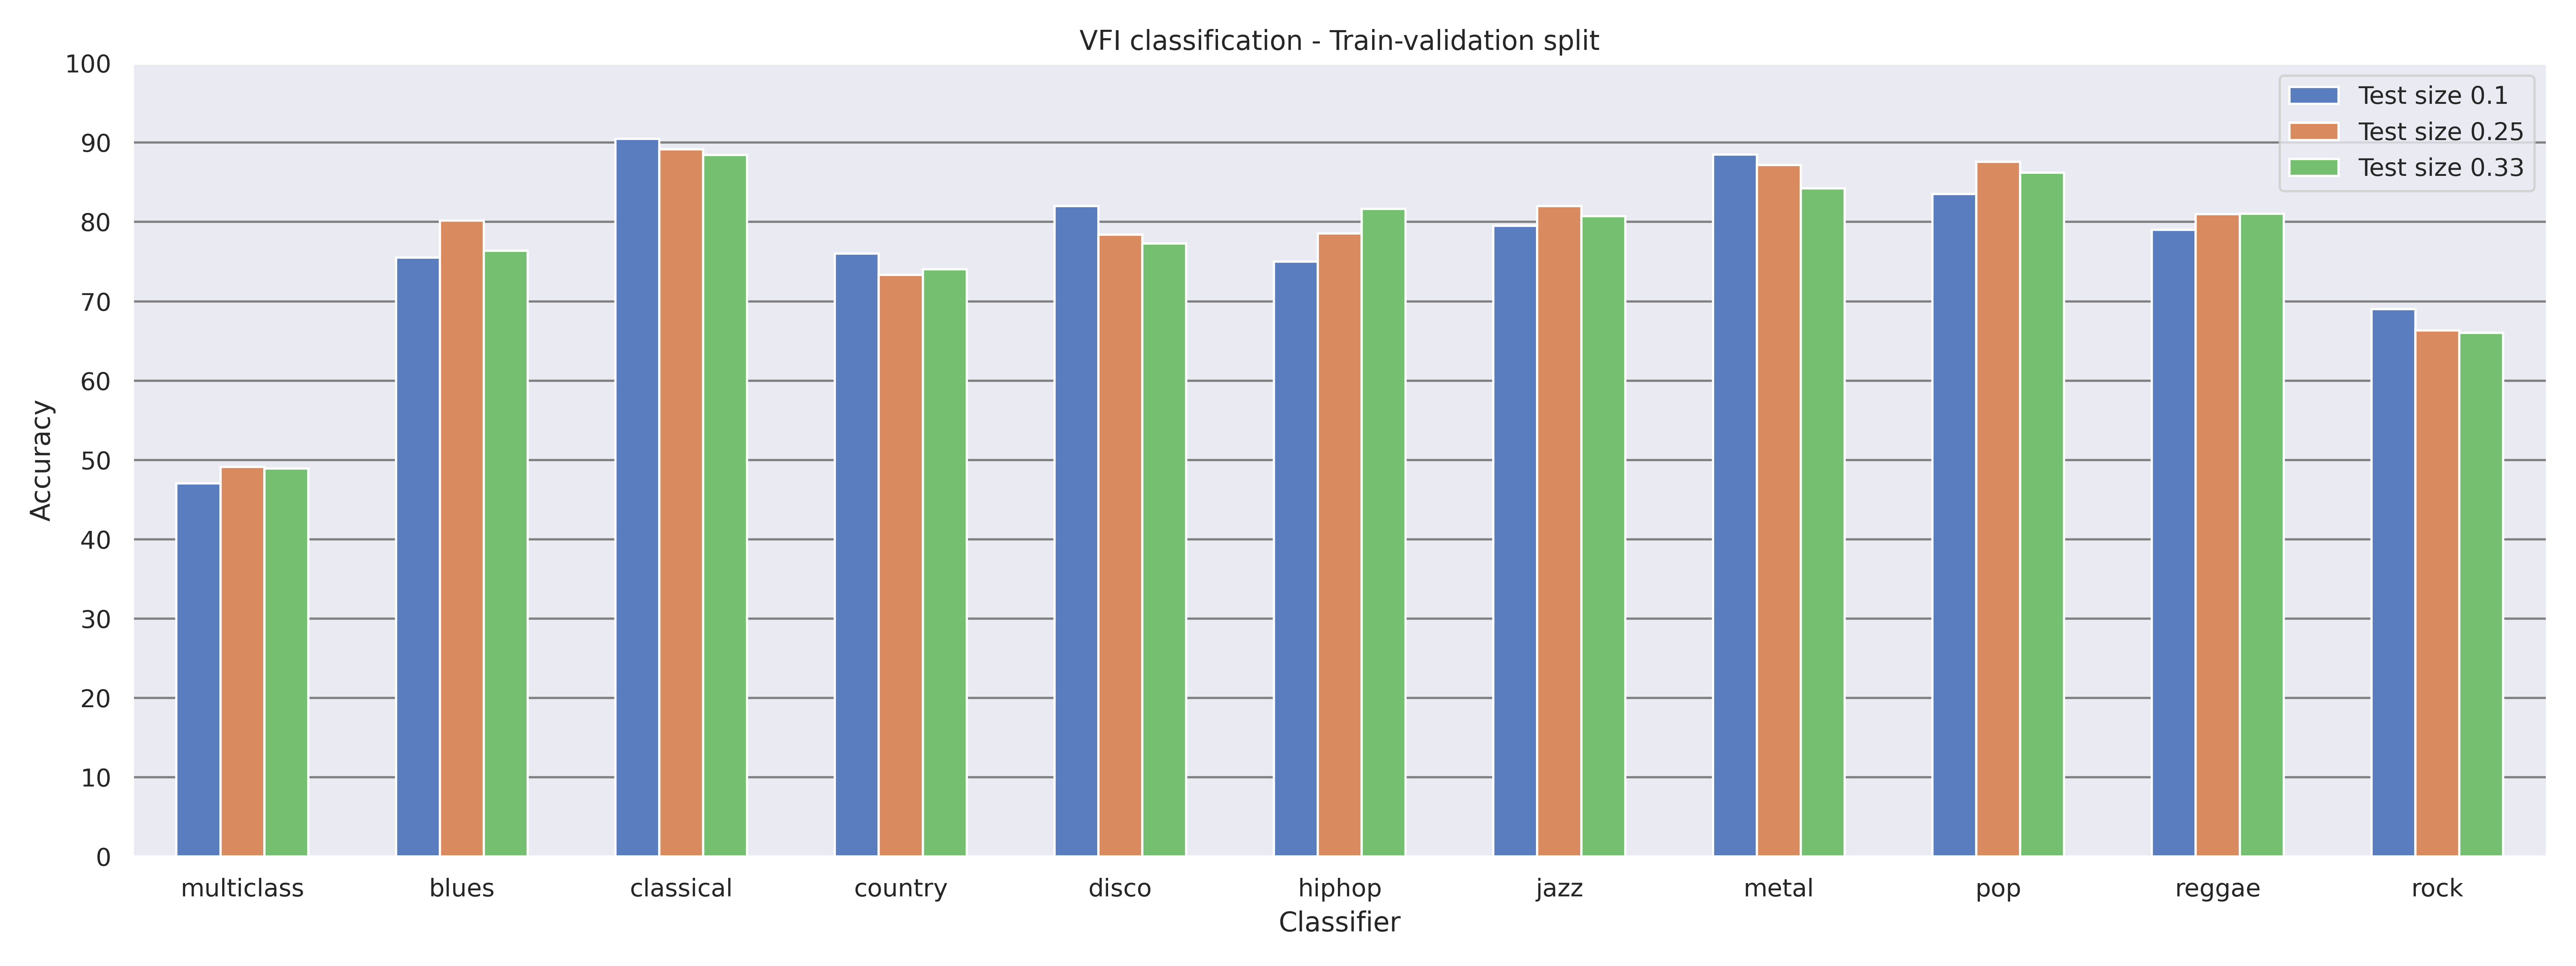
\includegraphics[width=\textwidth]{Figures/vfi_s.png}
    \caption{Accuracy of the VFI classifier with the train-validation split.}
    \label{fig:vfis}
\end{figure}

\begin{figure}[H]
    \centering
    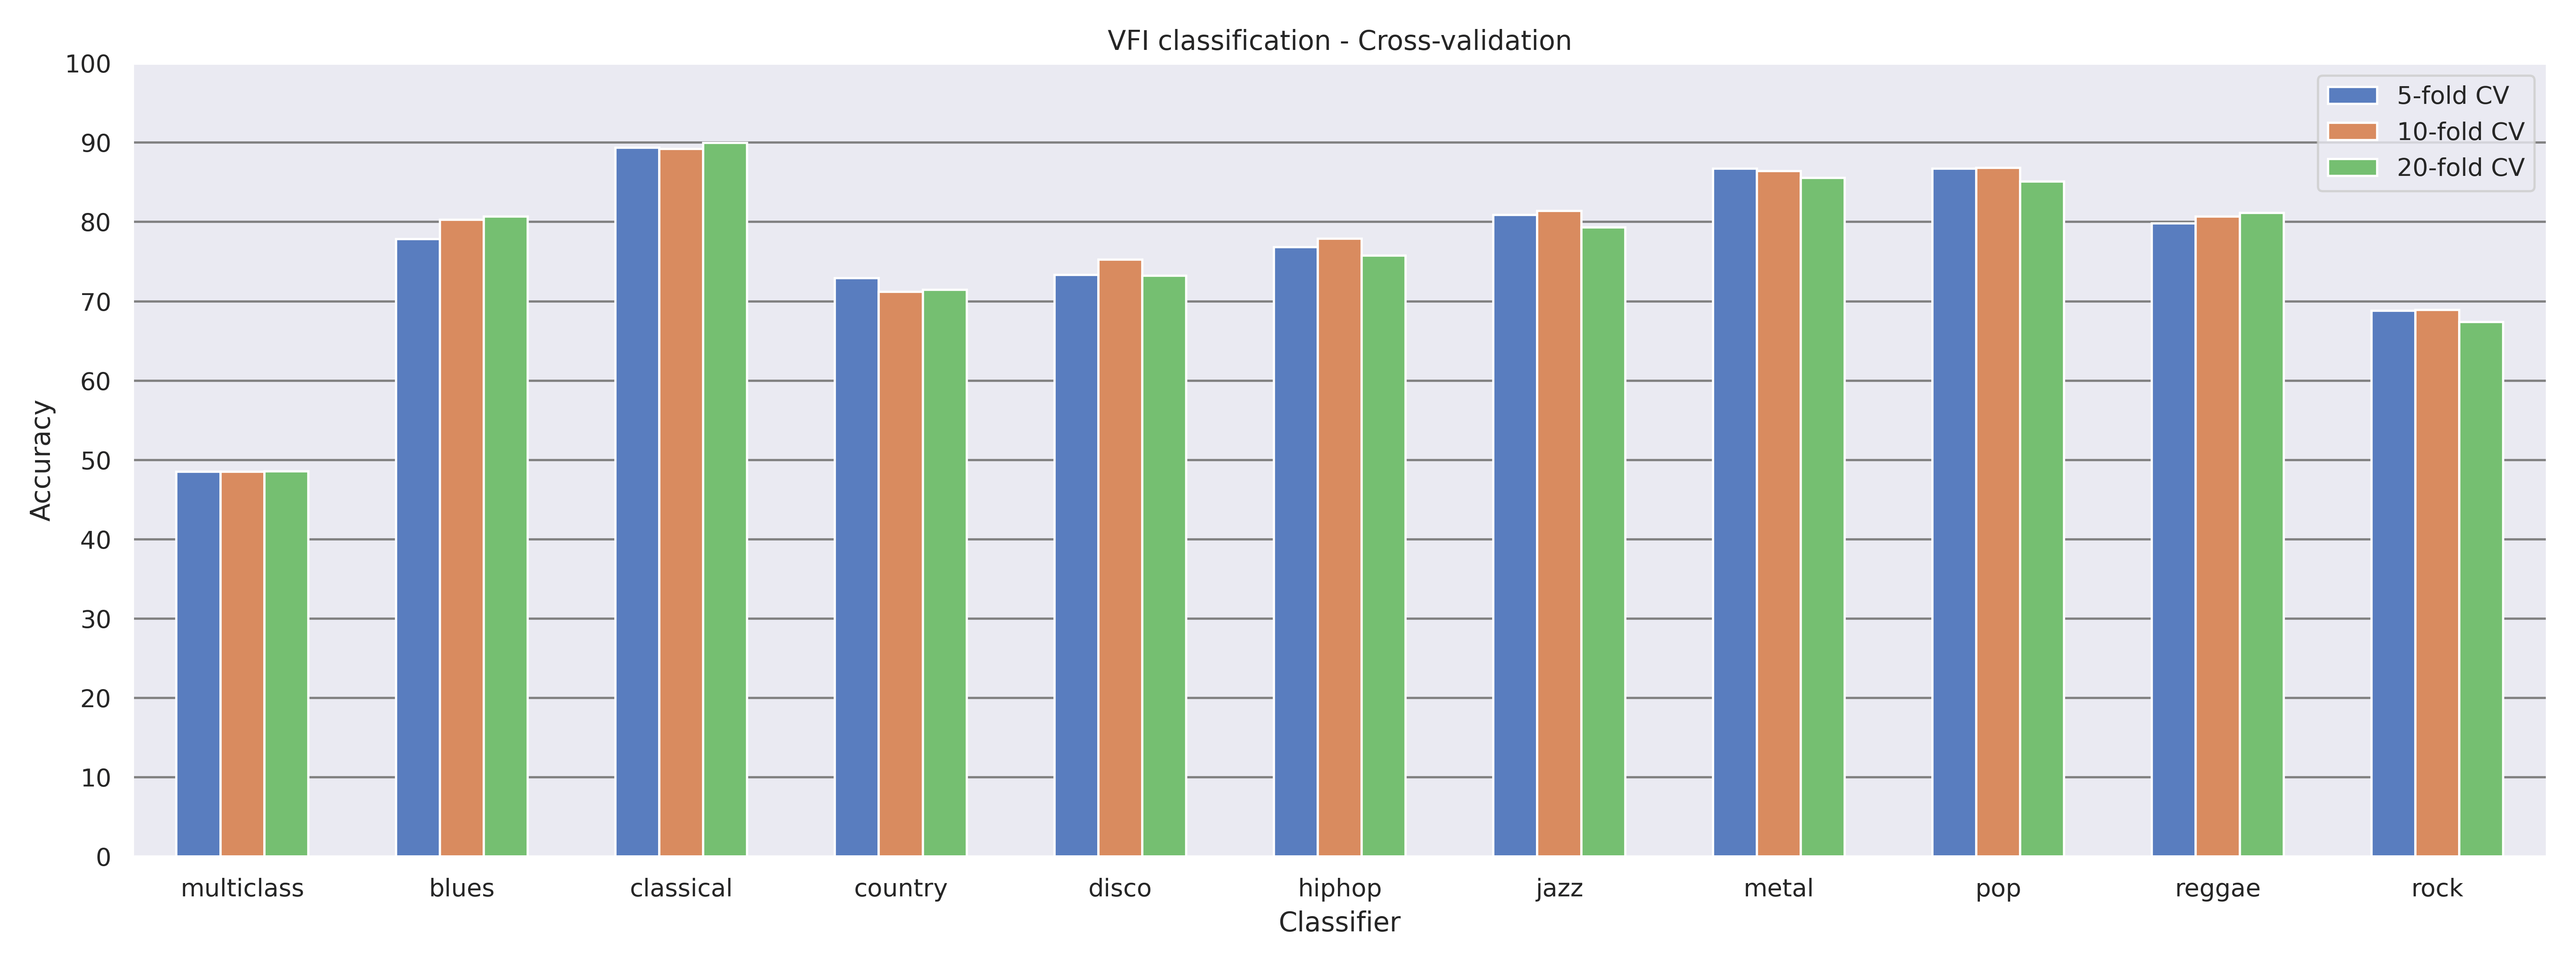
\includegraphics[width=\textwidth]{Figures/vfi_d.png}
    \caption{Accuracy of the VFI classifier with K-fold cross-validation.}
    \label{fig:vfid}
\end{figure}

VFI is a very similar model w.r.t. Naive Bayes, therefore we expected a similar performance. 
This is confirmed by our tests since we can easily see that the performance of VFI is very bad in the case of the multi-class classification problem and it is very good in the case of a simpler problem like classical music classification.

The following is the confusion matrix of the multi-class VFI classifier.

\begin{figure}[H]
    \centering
    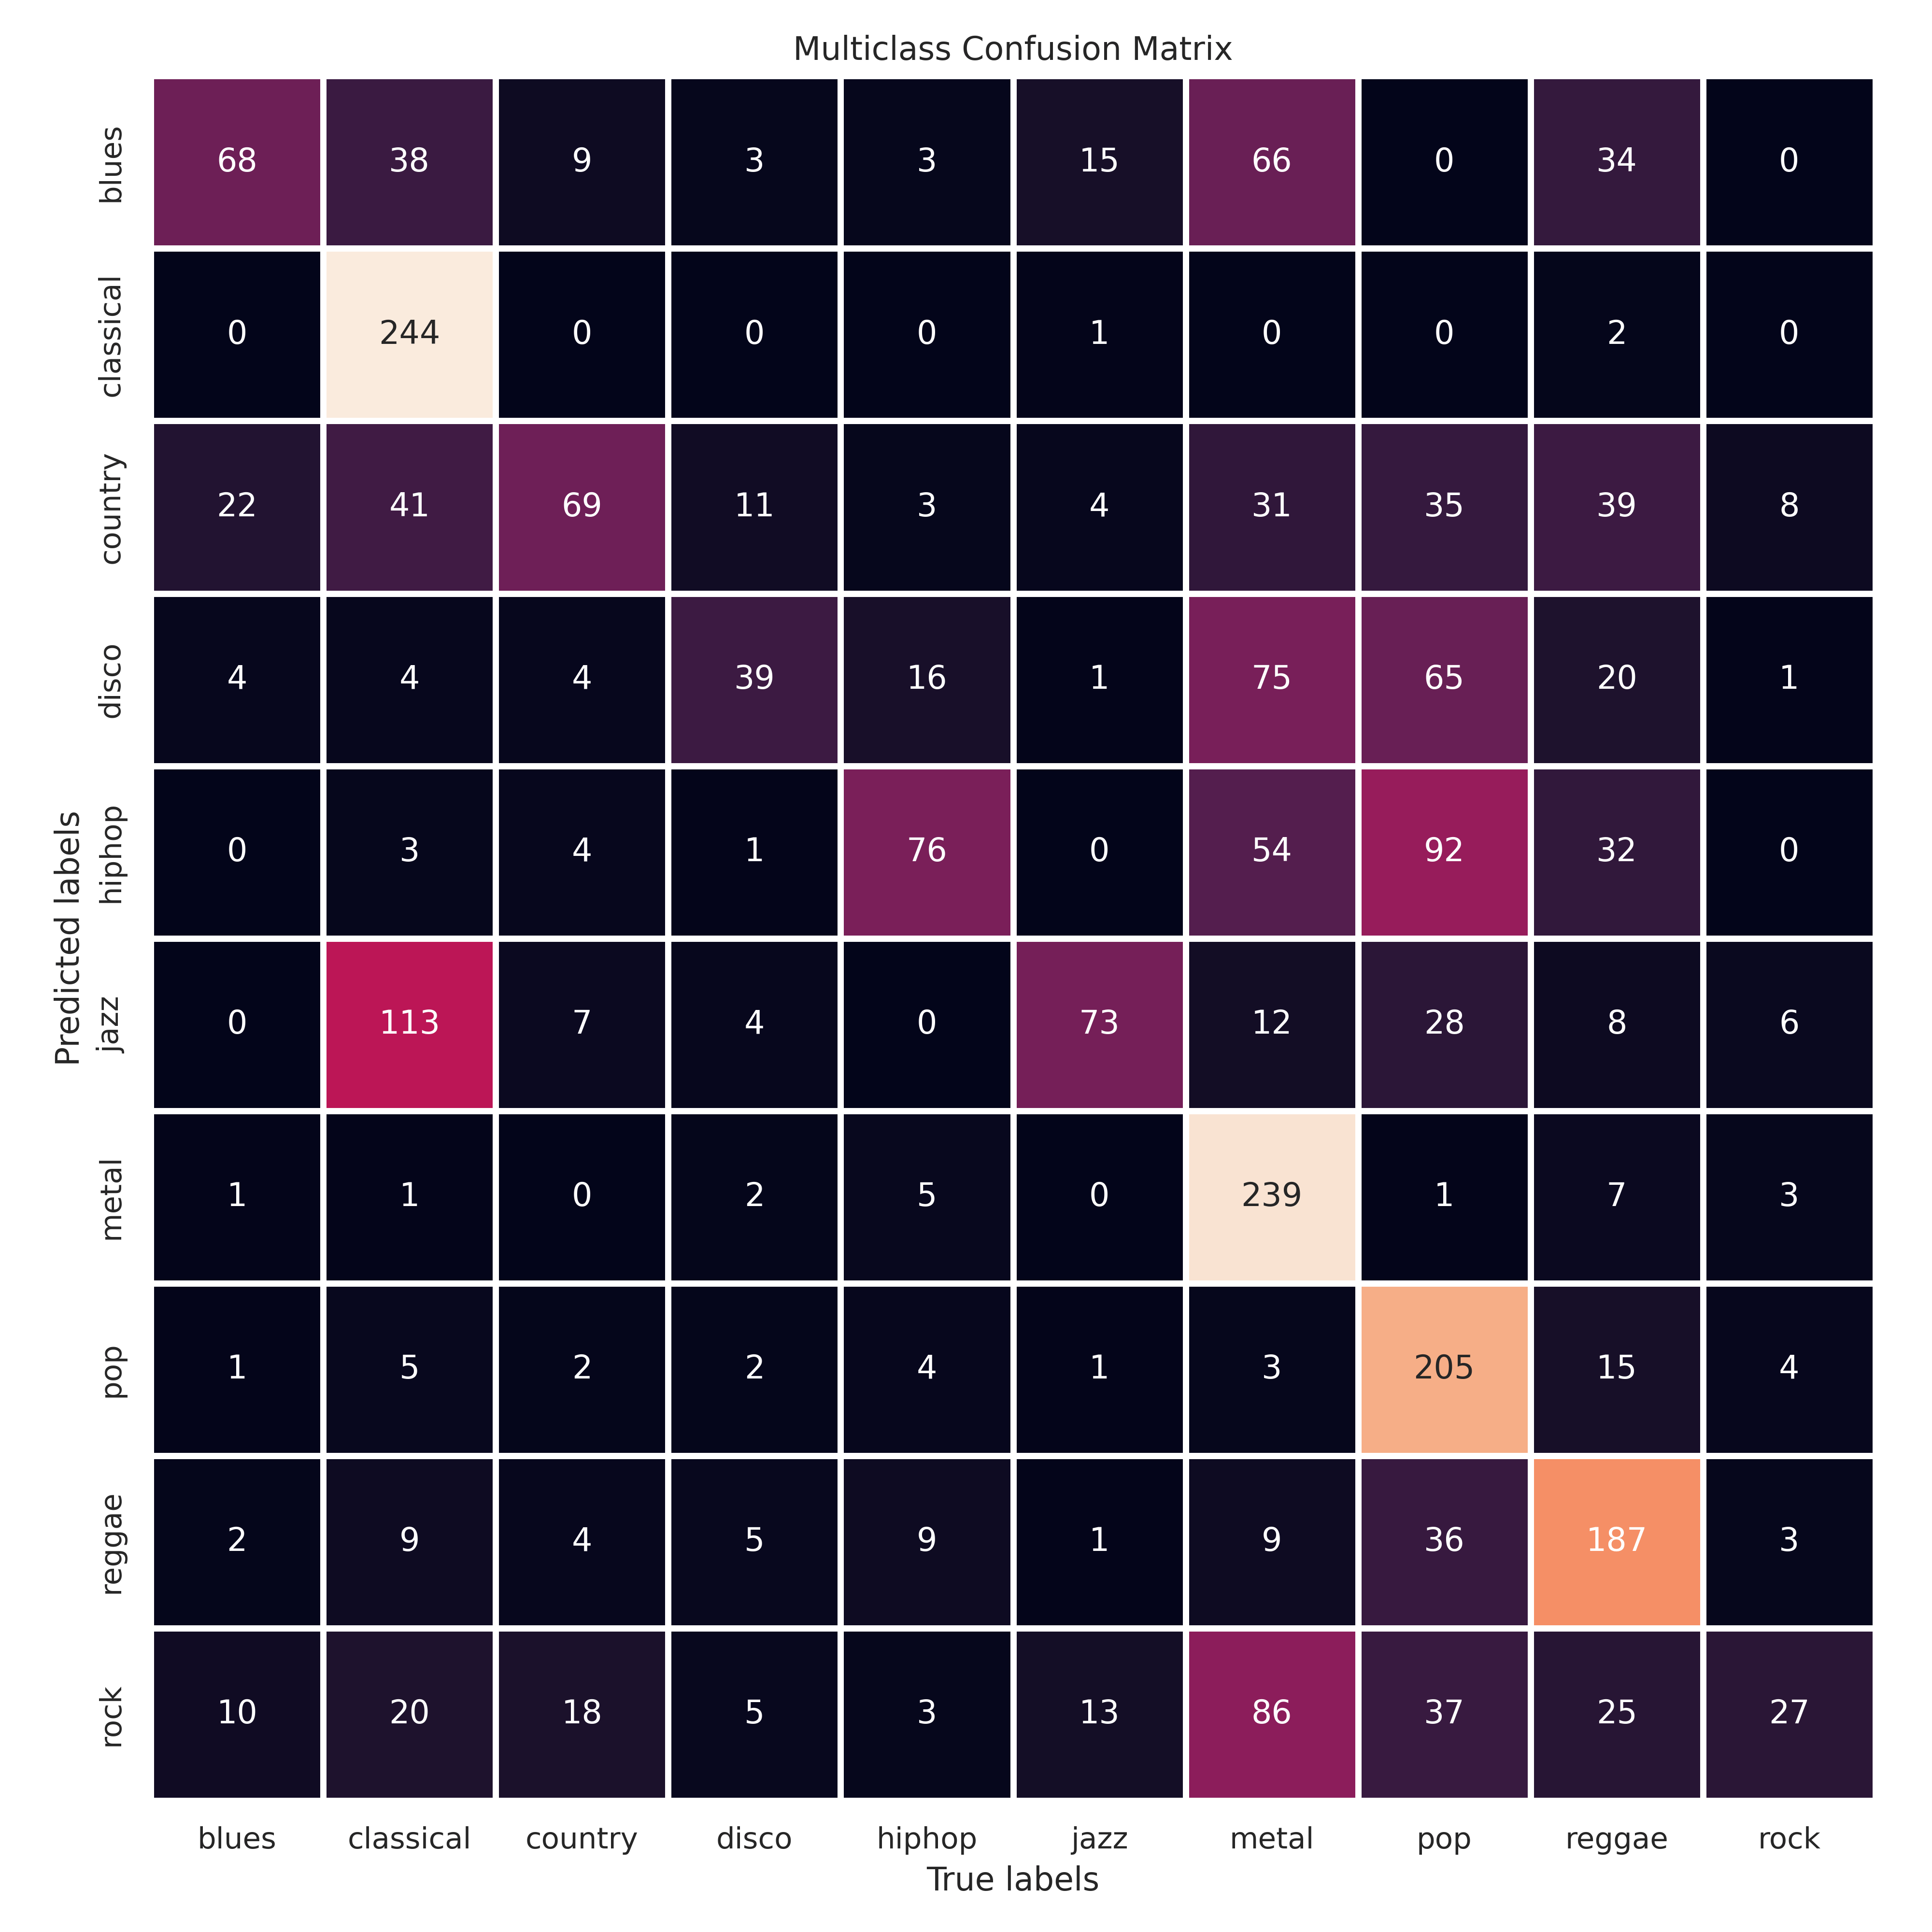
\includegraphics[width=0.7\textwidth]{Figures/vfi_m.png}
    \caption{Confusion matrix of the multi-class VFI classifier.}
    \label{fig:vfim}
\end{figure}

\pagebreak


\section{CART Decision Trees}
\label{sec:dtree}%
Decision Trees (DTs) are a non-parametric supervised learning method used for classification and regression. DTs are able to predict the value of a target variable by learning simple decision rules inferred from the data features. DTs are also simple to understand and interpret.

In our analysis, we used an implementation of decision trees known as CART (Classification and Regression Trees). CART constructs binary trees using the feature and the threshold that yield the largest information gain at each node. The code is provided by the library \textit{scikit-learn} \cite{scikit-learn}. 
Every step of this analysis is reported in the notebook \textit{CART\_DT.ipynb}.

Decision trees can work with a categorical target variable and do not require normalizing the data, therefore with this model, the pre-processing required is minimal.  

In the following charts, we can see the accuracy of the multi-class classifier and of the binary classifiers with different sizes of the train-validation split and with a different number of folds for the K-fold cross-validation.

\begin{figure}[H]
    \centering
    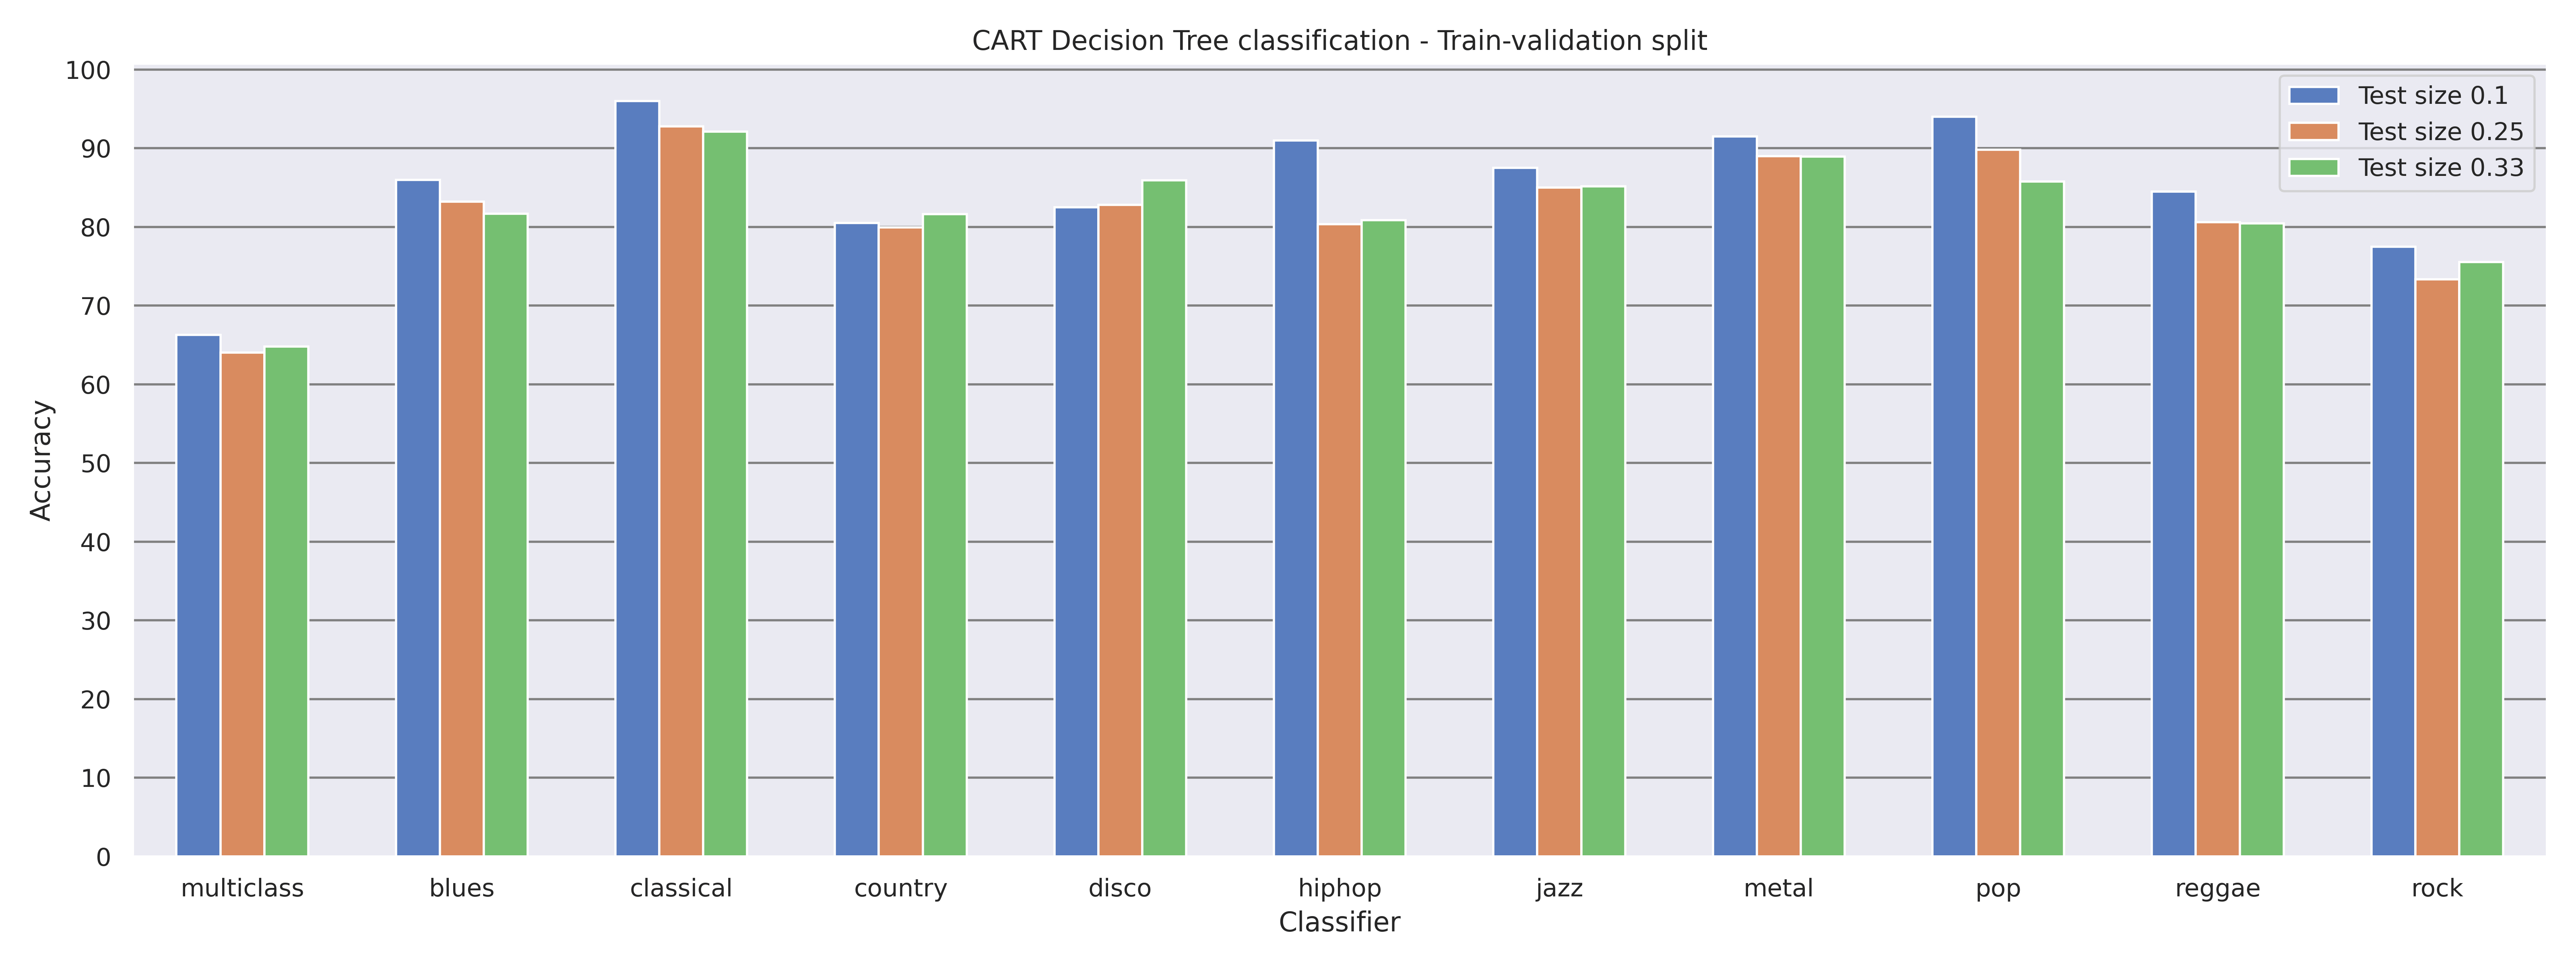
\includegraphics[width=\textwidth]{Figures/dtree_s.png}
    \caption{Accuracy of the CART DT classifier with the train-validation split.}
    \label{fig:dtrees}
\end{figure}

\begin{figure}[H]
    \centering
    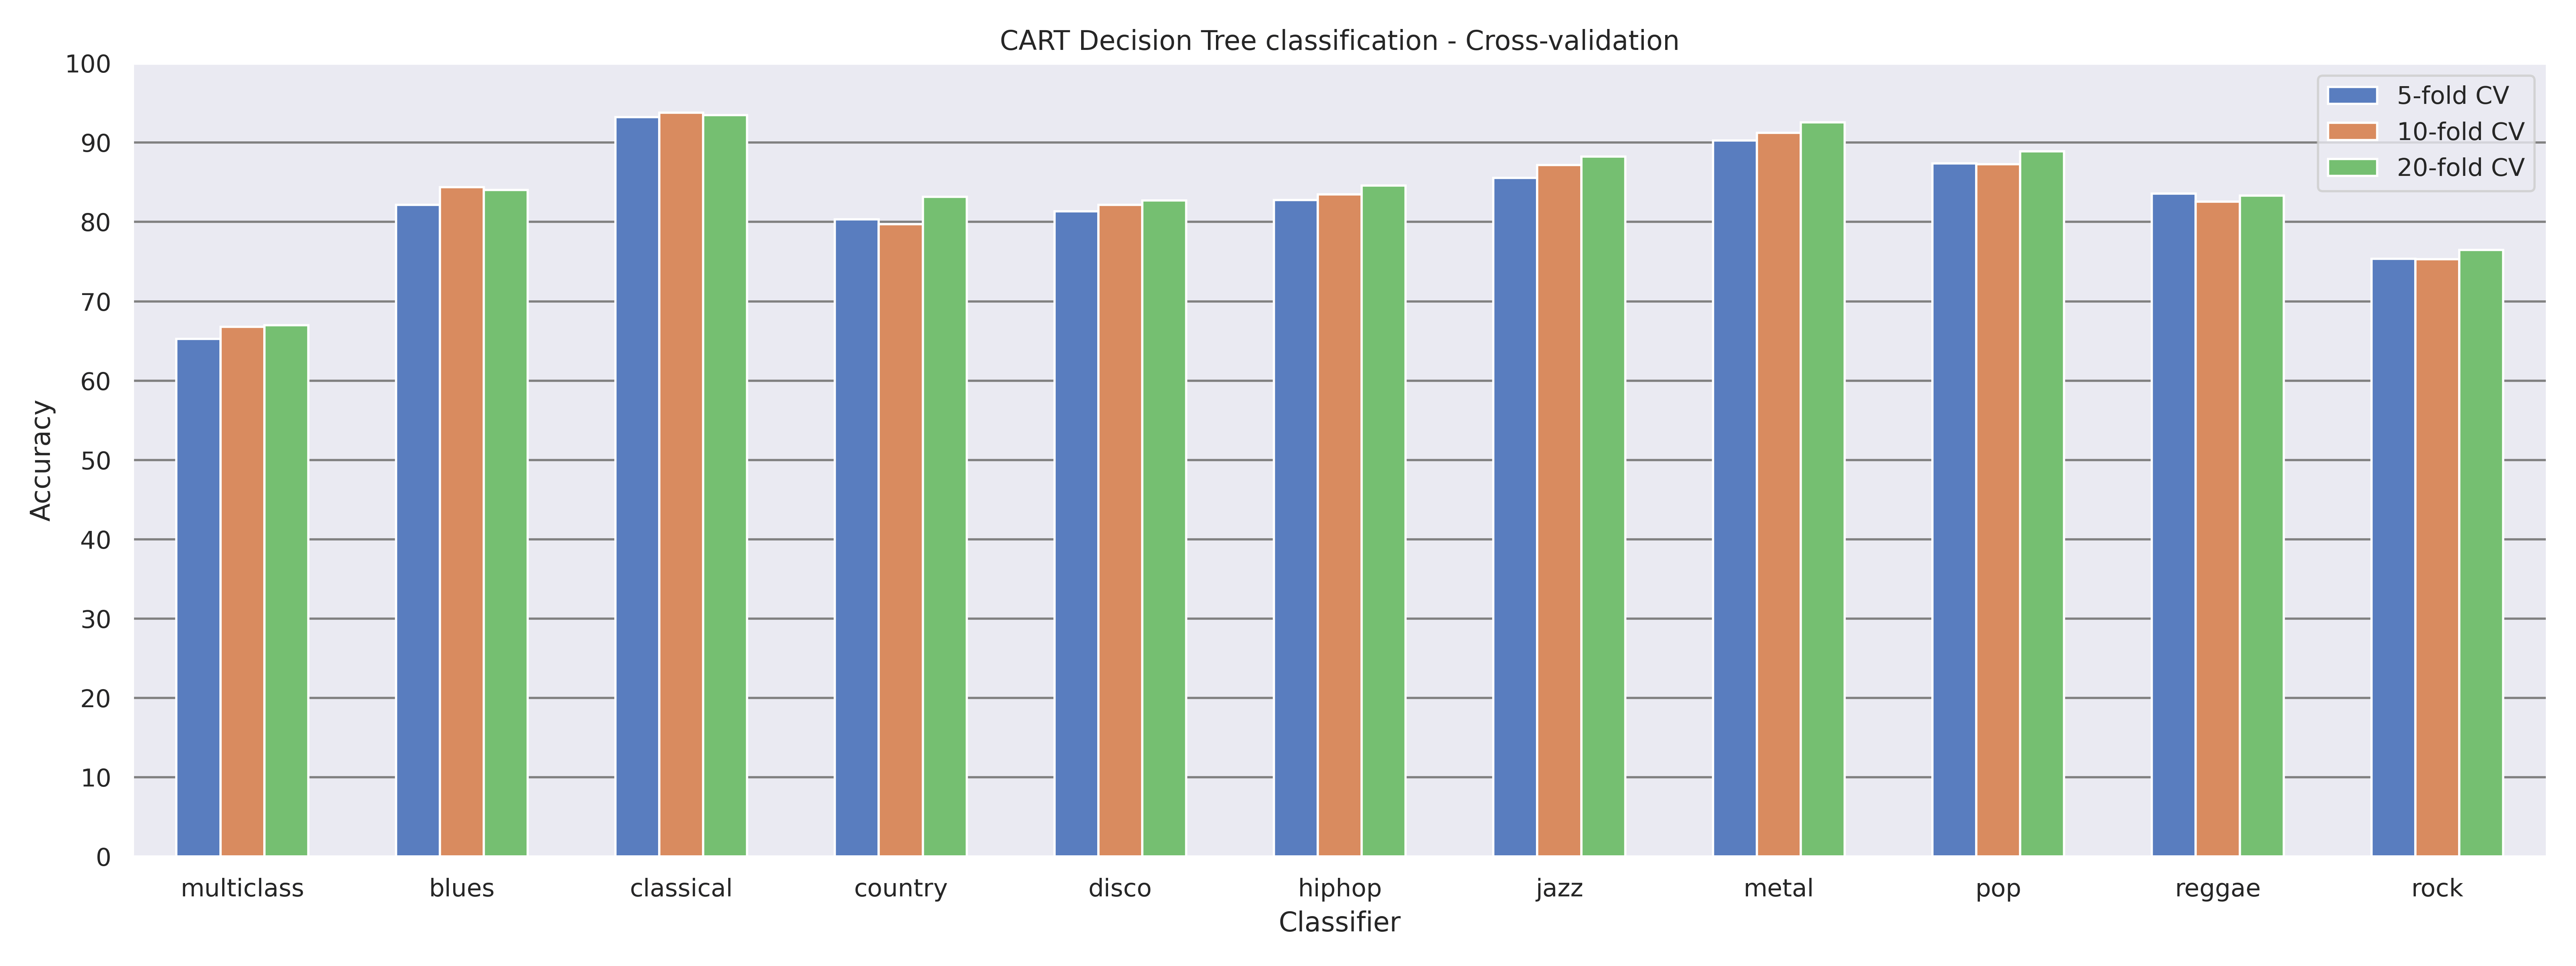
\includegraphics[width=\textwidth]{Figures/dtree_d.png}
    \caption{Accuracy of the CART DT classifier with K-fold cross-validation.}
    \label{fig:dtreed}
\end{figure}

We are starting to see better overall accuracy. In fact, decision trees are known to offer good performance despite their short training phase. Furthermore, DTs are non-parametric models, meaning that they do not make any assumption about the distribution of the data and therefore are able to capture complex relationships between the variables.

The following is the confusion matrix of the multi-class CART DT classifier.

\begin{figure}[H]
    \centering
    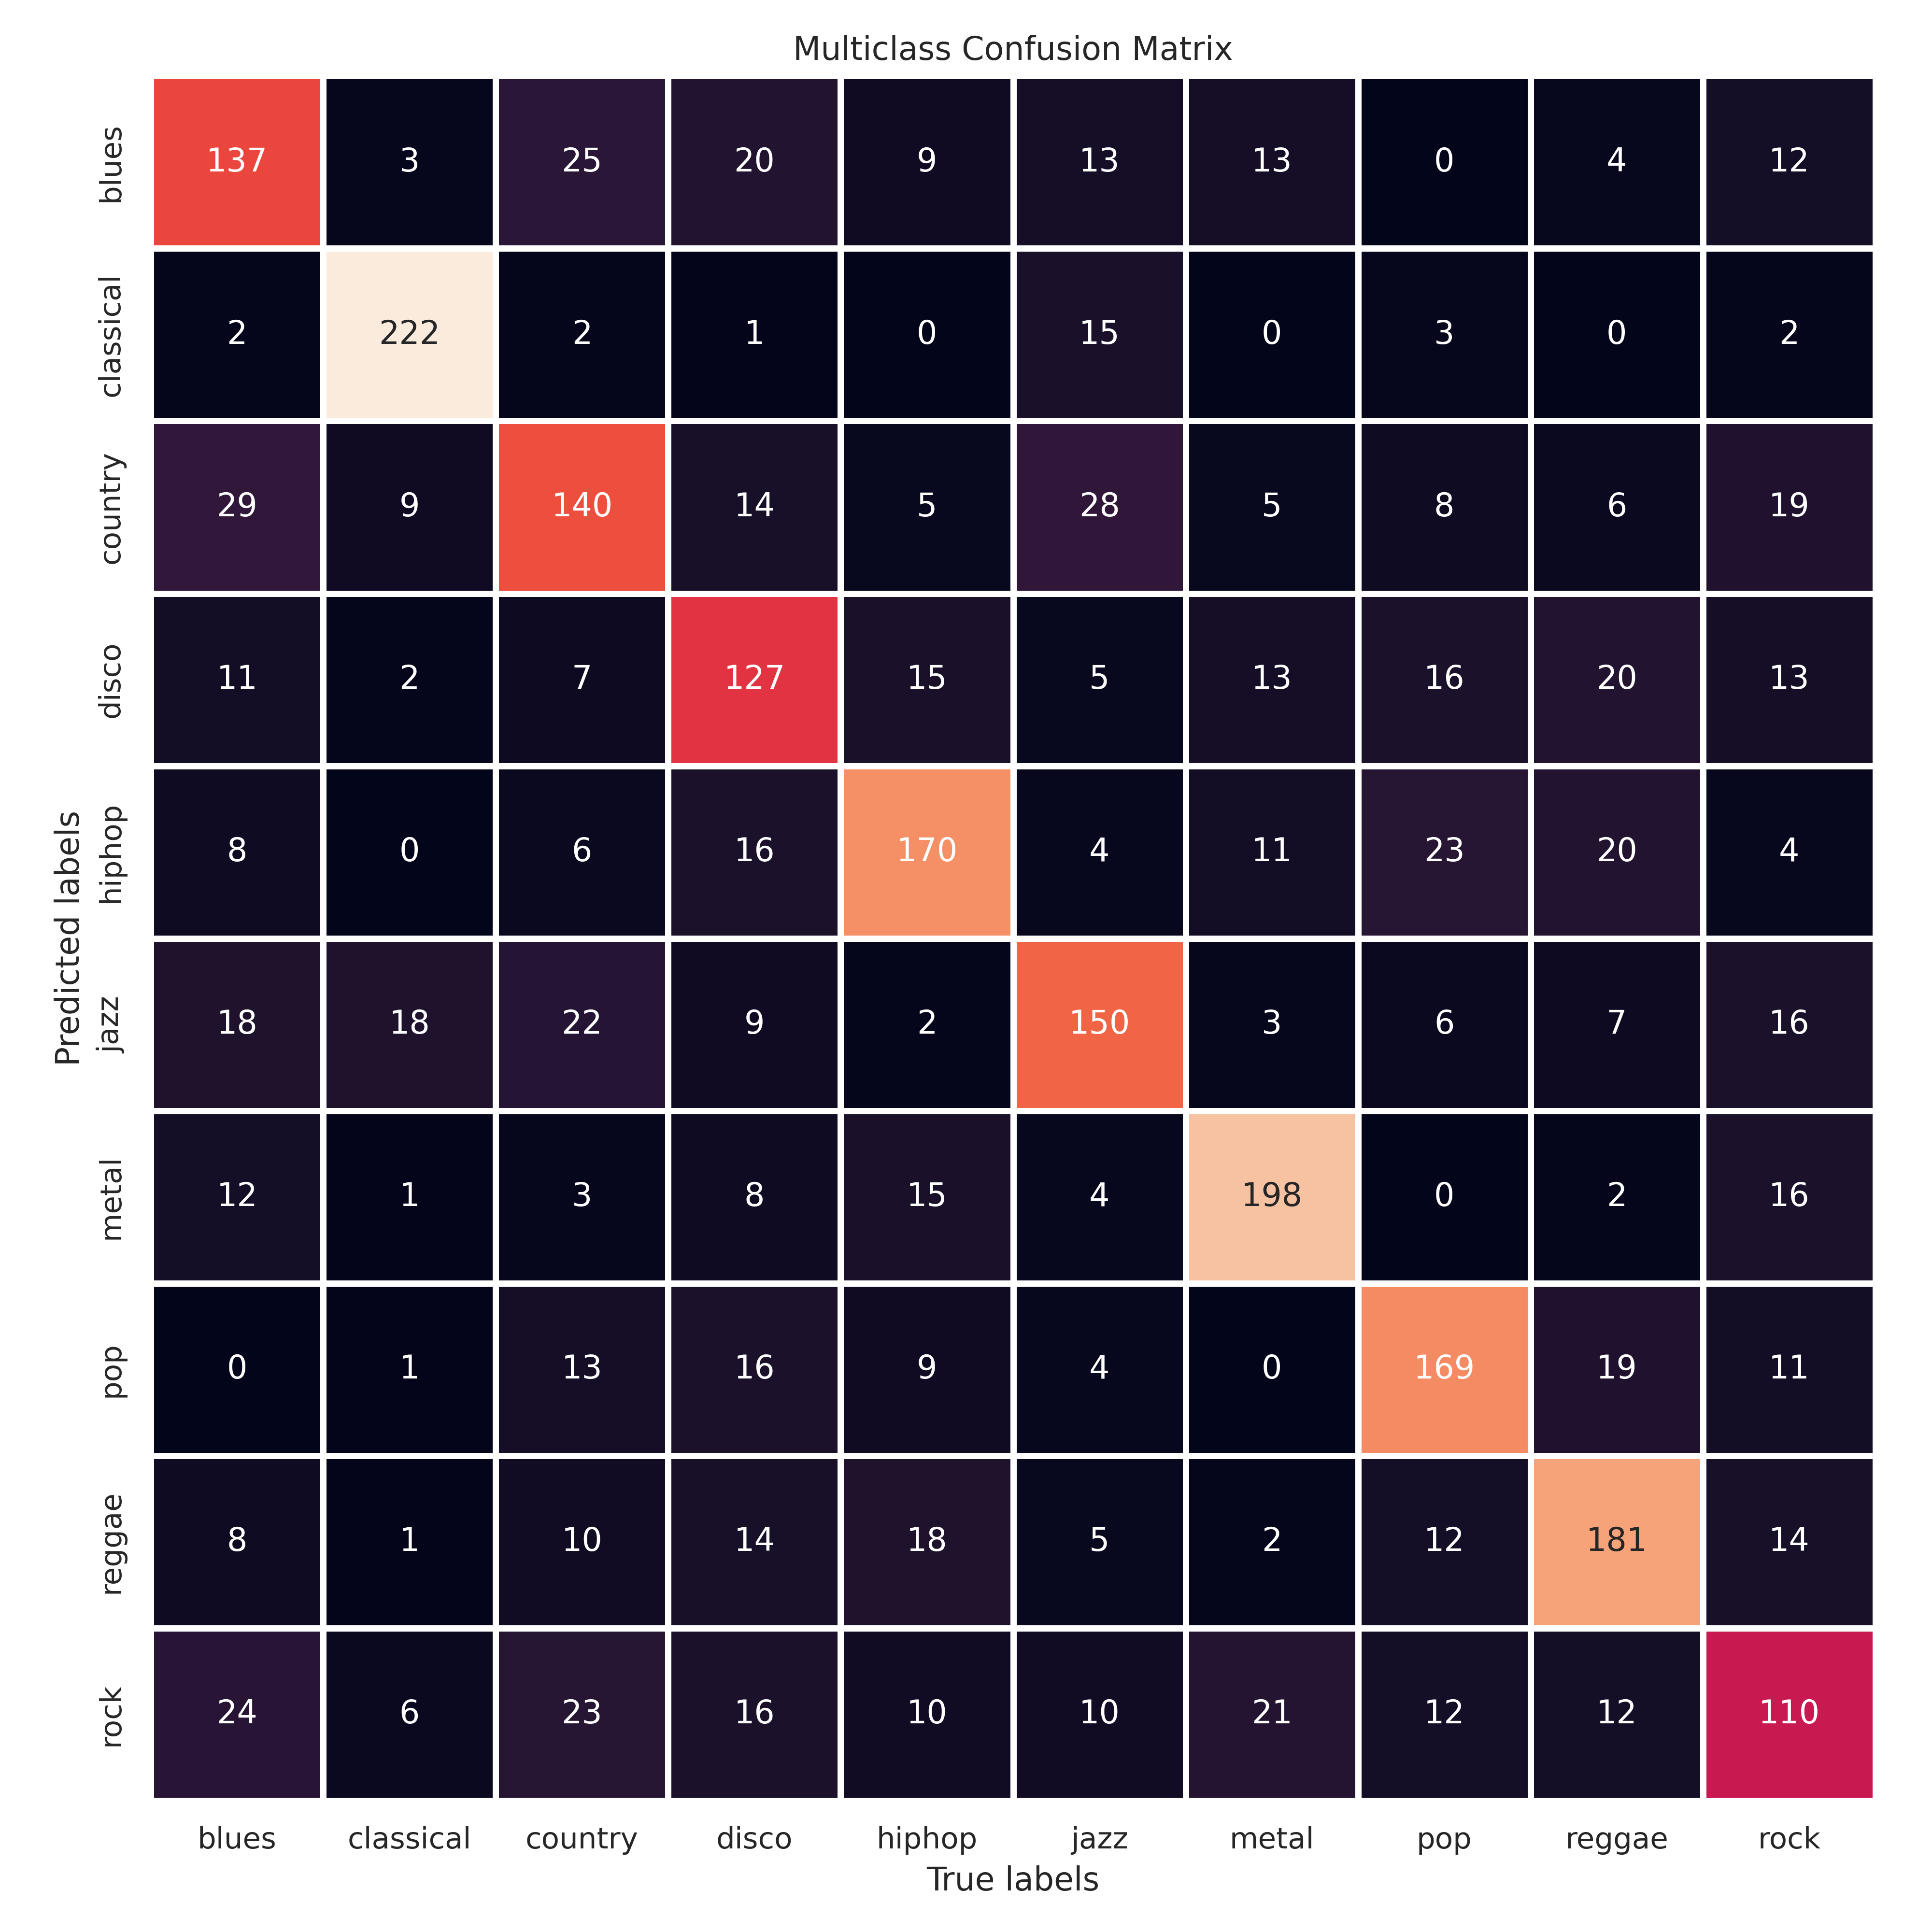
\includegraphics[width=0.7\textwidth]{Figures/dtree_m.png}
    \caption{Confusion matrix of the multi-class CART DT classifier.}
    \label{fig:dtreem}
\end{figure}

\pagebreak


\section{K-Nearest Neighbors}
\label{sec:knn}%
Neighbors-based classification is a type of instance-based learning, meaning that it does not attempt to construct a general internal model, but simply stores instances of the training data. Classification is computed through a simple majority vote of the nearest neighbors of each point.

In our analysis, we used the K-Nearest Neighbors (K-NN) classifier, which implements learning based on the nearest neighbors of each query point. The code is provided by the library \textit{scikit-learn} \cite{scikit-learn}. 
Every step of this analysis is reported in the notebook \textit{KNN.ipynb}.

It is known that the optimal choice of the value of $k$ is highly data-dependent: in general, a larger $k$ suppresses the effects of noise but makes the classification boundaries less distinct.

On the other hand, there are two possible choices for the weights:

\begin{itemize}
    \item \textit{uniform}: assigns uniform weights to each neighbor.
    \item \textit{distance}: assigns weights proportional to the inverse of the distance from the query point. 
\end{itemize}

Then, the value assigned to a query point is computed from a simple majority vote of the nearest neighbors.

This means that this time the model we are working with has some hyper-parameters. In order to find the best-performing model in our scenario, we will try all the combinations of the following two hyper-parameters. Note that we can afford this brute force approach since there are just two hyper-parameters that can only take a small set of values and since the time required to train each model is low.

K-NN can work with a categorical target variable but performs better when the data is normalized, therefore also in this case we will normalize the data set through standardization.

We have trained a different model for each combination of two hyper-parameters and compared them with one another using 20-fold cross-validation. The best model is the one with the highest average accuracy. 

In the following chart, we can see the performance of all the models trained to solve the multi-class classification problem. We did not attempt to train models with a number of neighbors higher than 20 since we noticed that in this specific case adding more neighbors was making the predictions worse.

\begin{figure}[H]
    \centering
    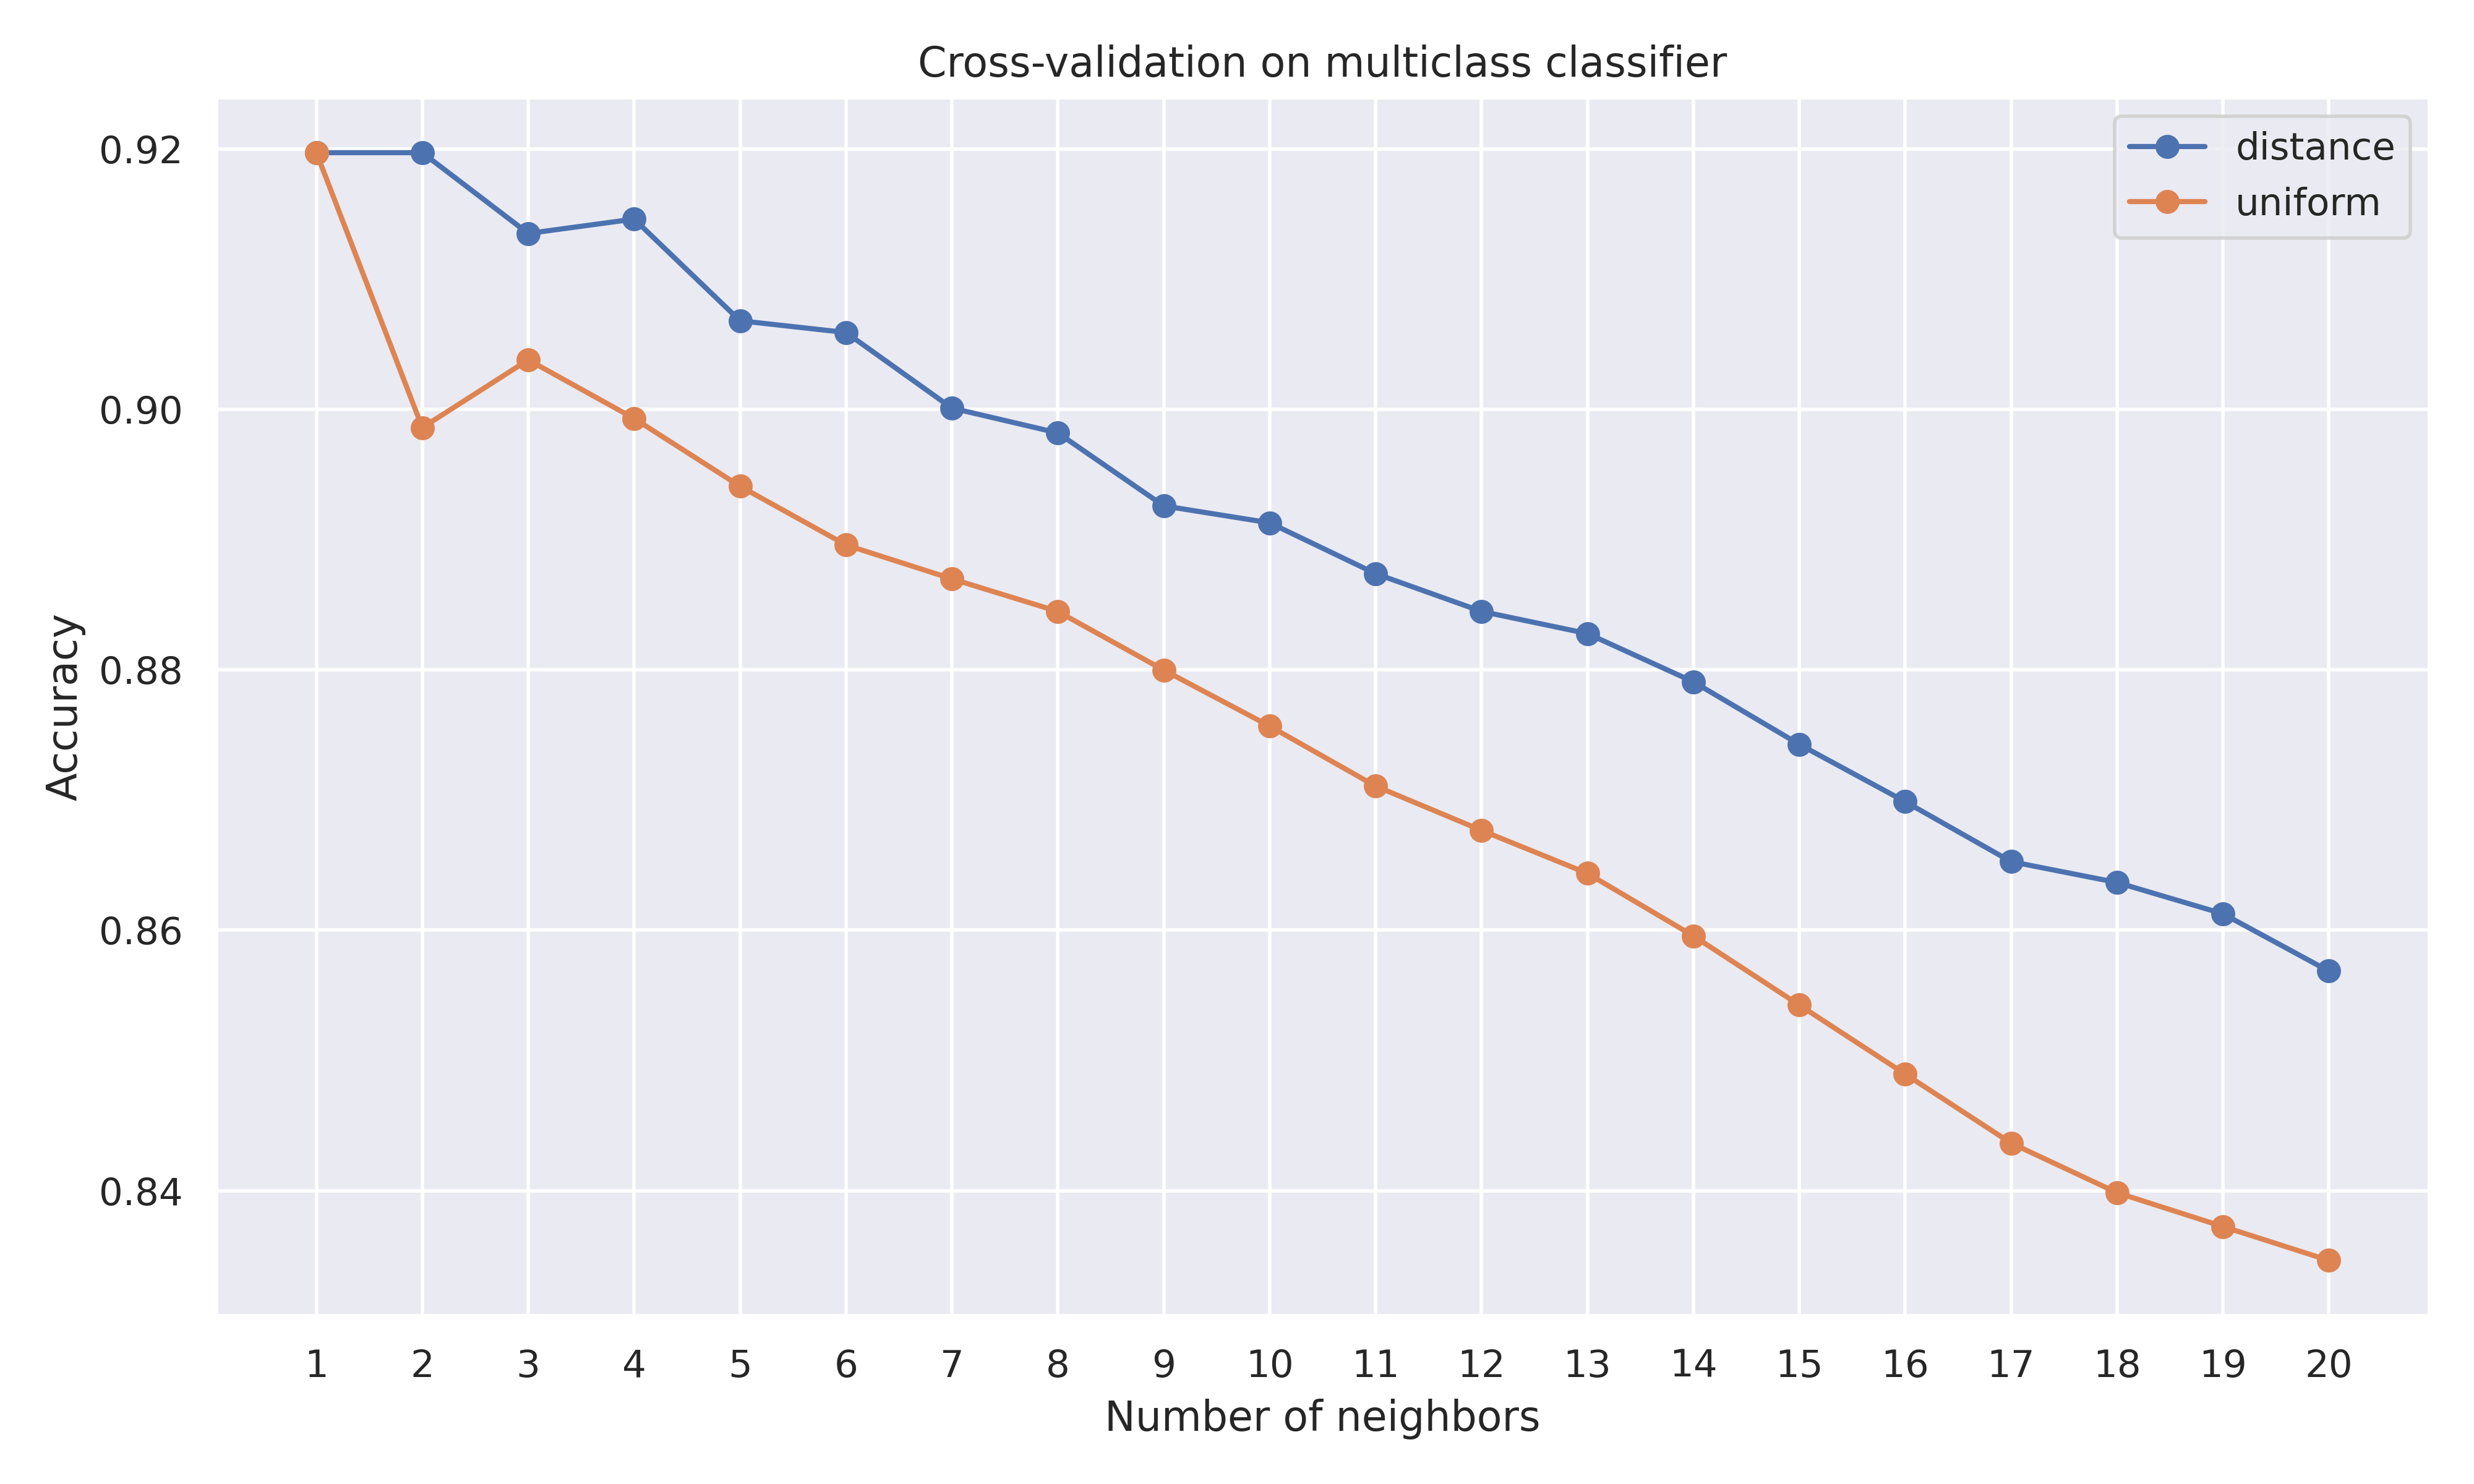
\includegraphics[width=0.8\textwidth]{Figures/knn_selection_m.png}
    \caption{Model selection results of K-NN multi-class.}
    \label{fig:knn_sel_m}
\end{figure}

In the following chart, we can see the performance of all the models trained to solve the binary classification problems. In this case, we limited the number of neighbors to 15 since adding more neighbors was not improving the performance. 

\begin{figure}[H]
    \centering
    \includegraphics[width=0.7\textwidth]{Figures/knn_selection_b.png}
    \caption{Model selection results of K-NN binary.}
    \label{fig:knn_sel_b}
\end{figure}

The following table reports the best hyper-parameters found for each one of the multi-class problem and the 10 binary problems:

\begin{table}[H]
    \centering 
    \begin{tabular}{|c | c c |}
    \hline
    \rowcolor{bluepoli!40} 
     Classification problem & Number of neighbors & Weights \T\B \\
    \hline \hline
    multi-class & 1 & distance   \T\B \\
    blues & 2 & uniform   \T\B \\
    classical & 1 & distance   \T\B \\
    country & 1 & uniform   \T\B \\
    disco & 2 & uniform   \T\B \\
    hip-hop & 2 & uniform   \T\B \\
    jazz & 2 & uniform   \T\B \\
    metal & 2 & uniform   \T\B \\
    pop & 4 & distance   \T\B \\
    reggae & 2 & uniform   \T\B \\
    rock & 2 & uniform   \T\B \\
    \hline
    \end{tabular}
    \\[10pt]
\end{table}

In the following charts, we can see the accuracy of the multi-class classifier and of the binary classifiers with different sizes of the train-validation split and with a different number of folds for the K-fold cross-validation. The models we are using are the ones with the hyper-parameters selected in the previous step.

\begin{figure}[H]
    \centering
    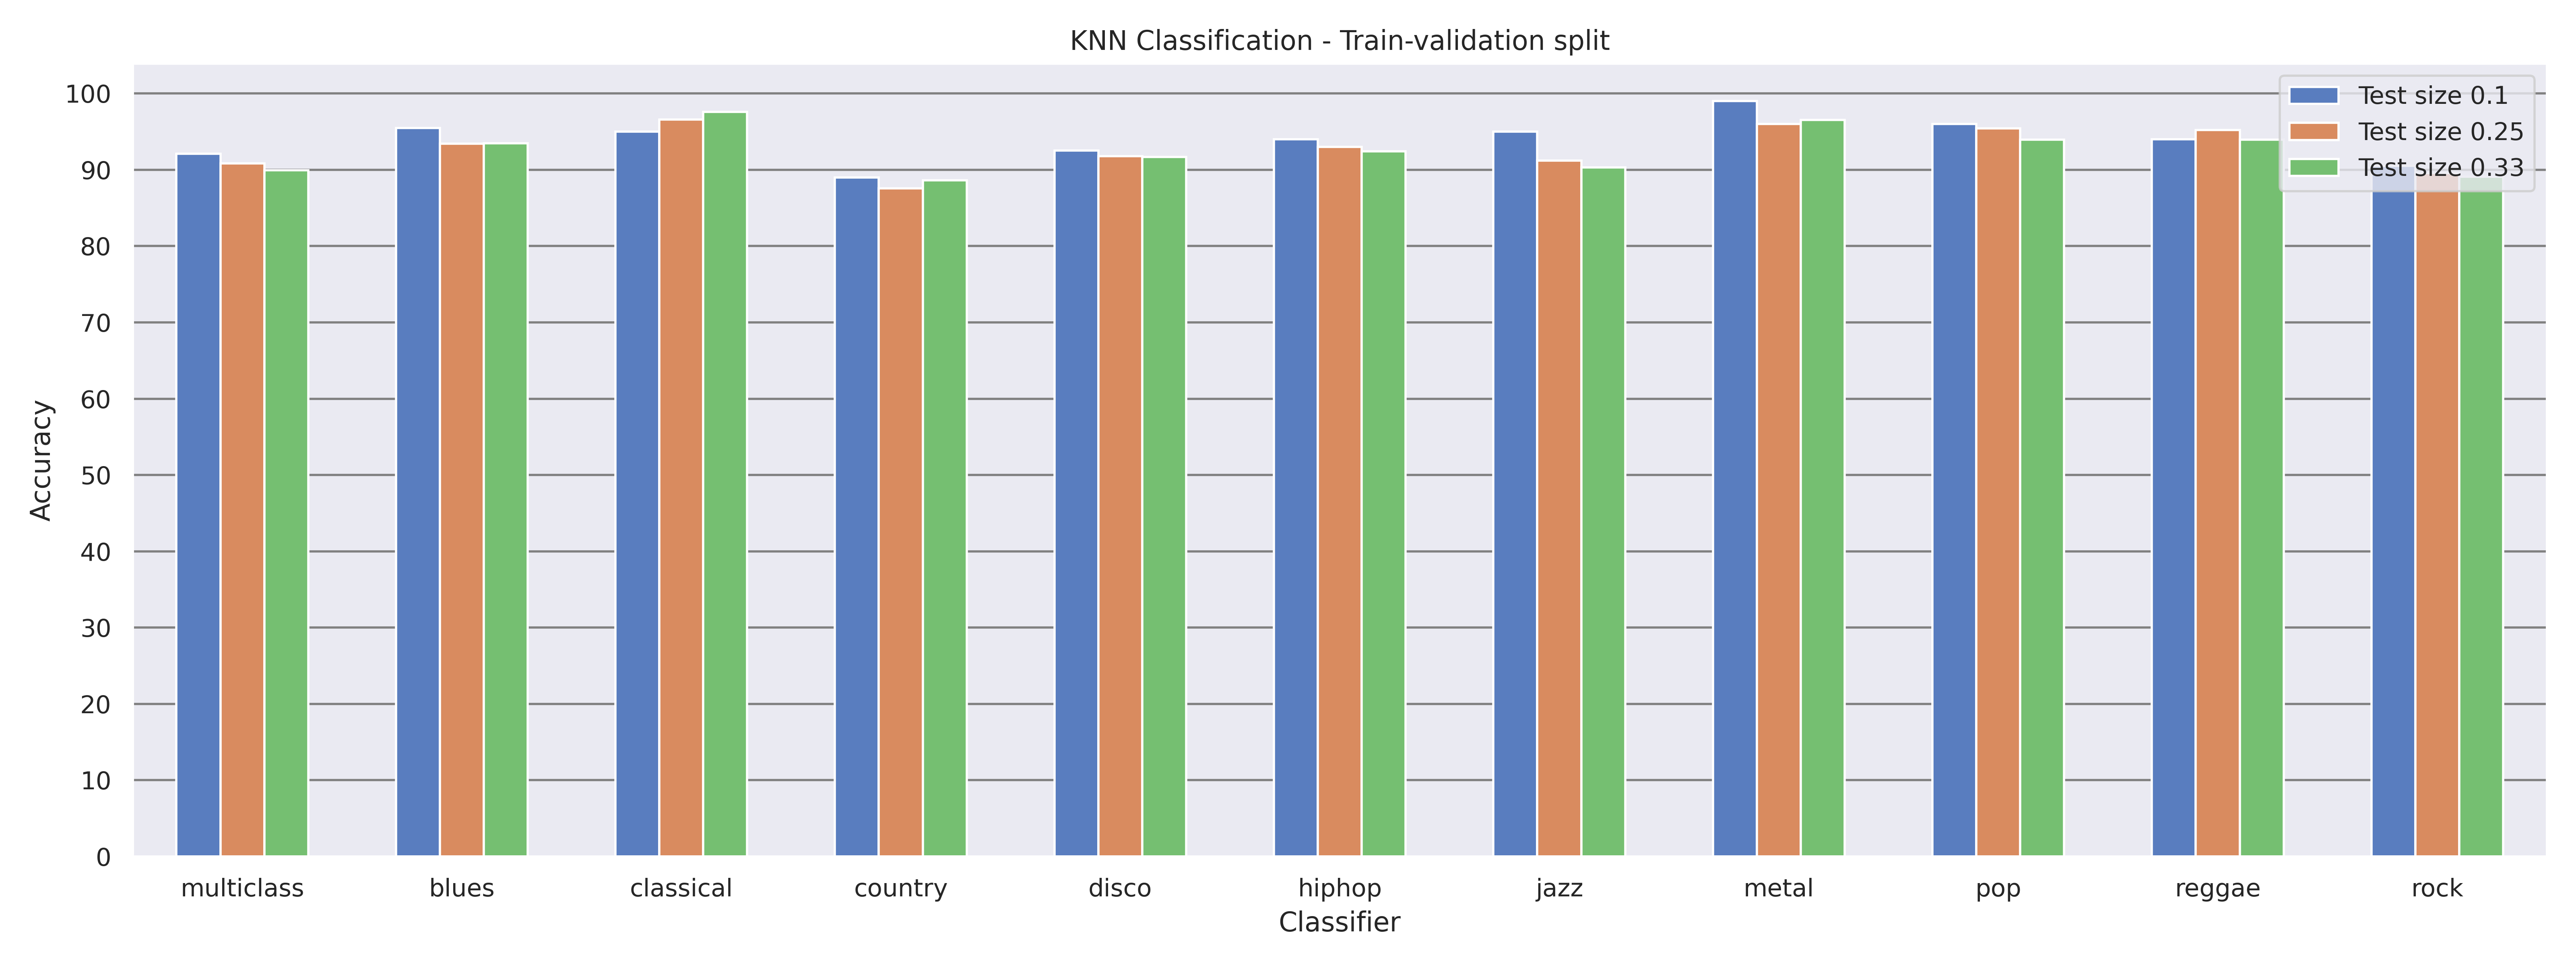
\includegraphics[width=\textwidth]{Figures/knn_s.png}
    \caption{Accuracy of the K-NN classifier with the train-validation split.}
    \label{fig:knns}
\end{figure}

\begin{figure}[H]
    \centering
    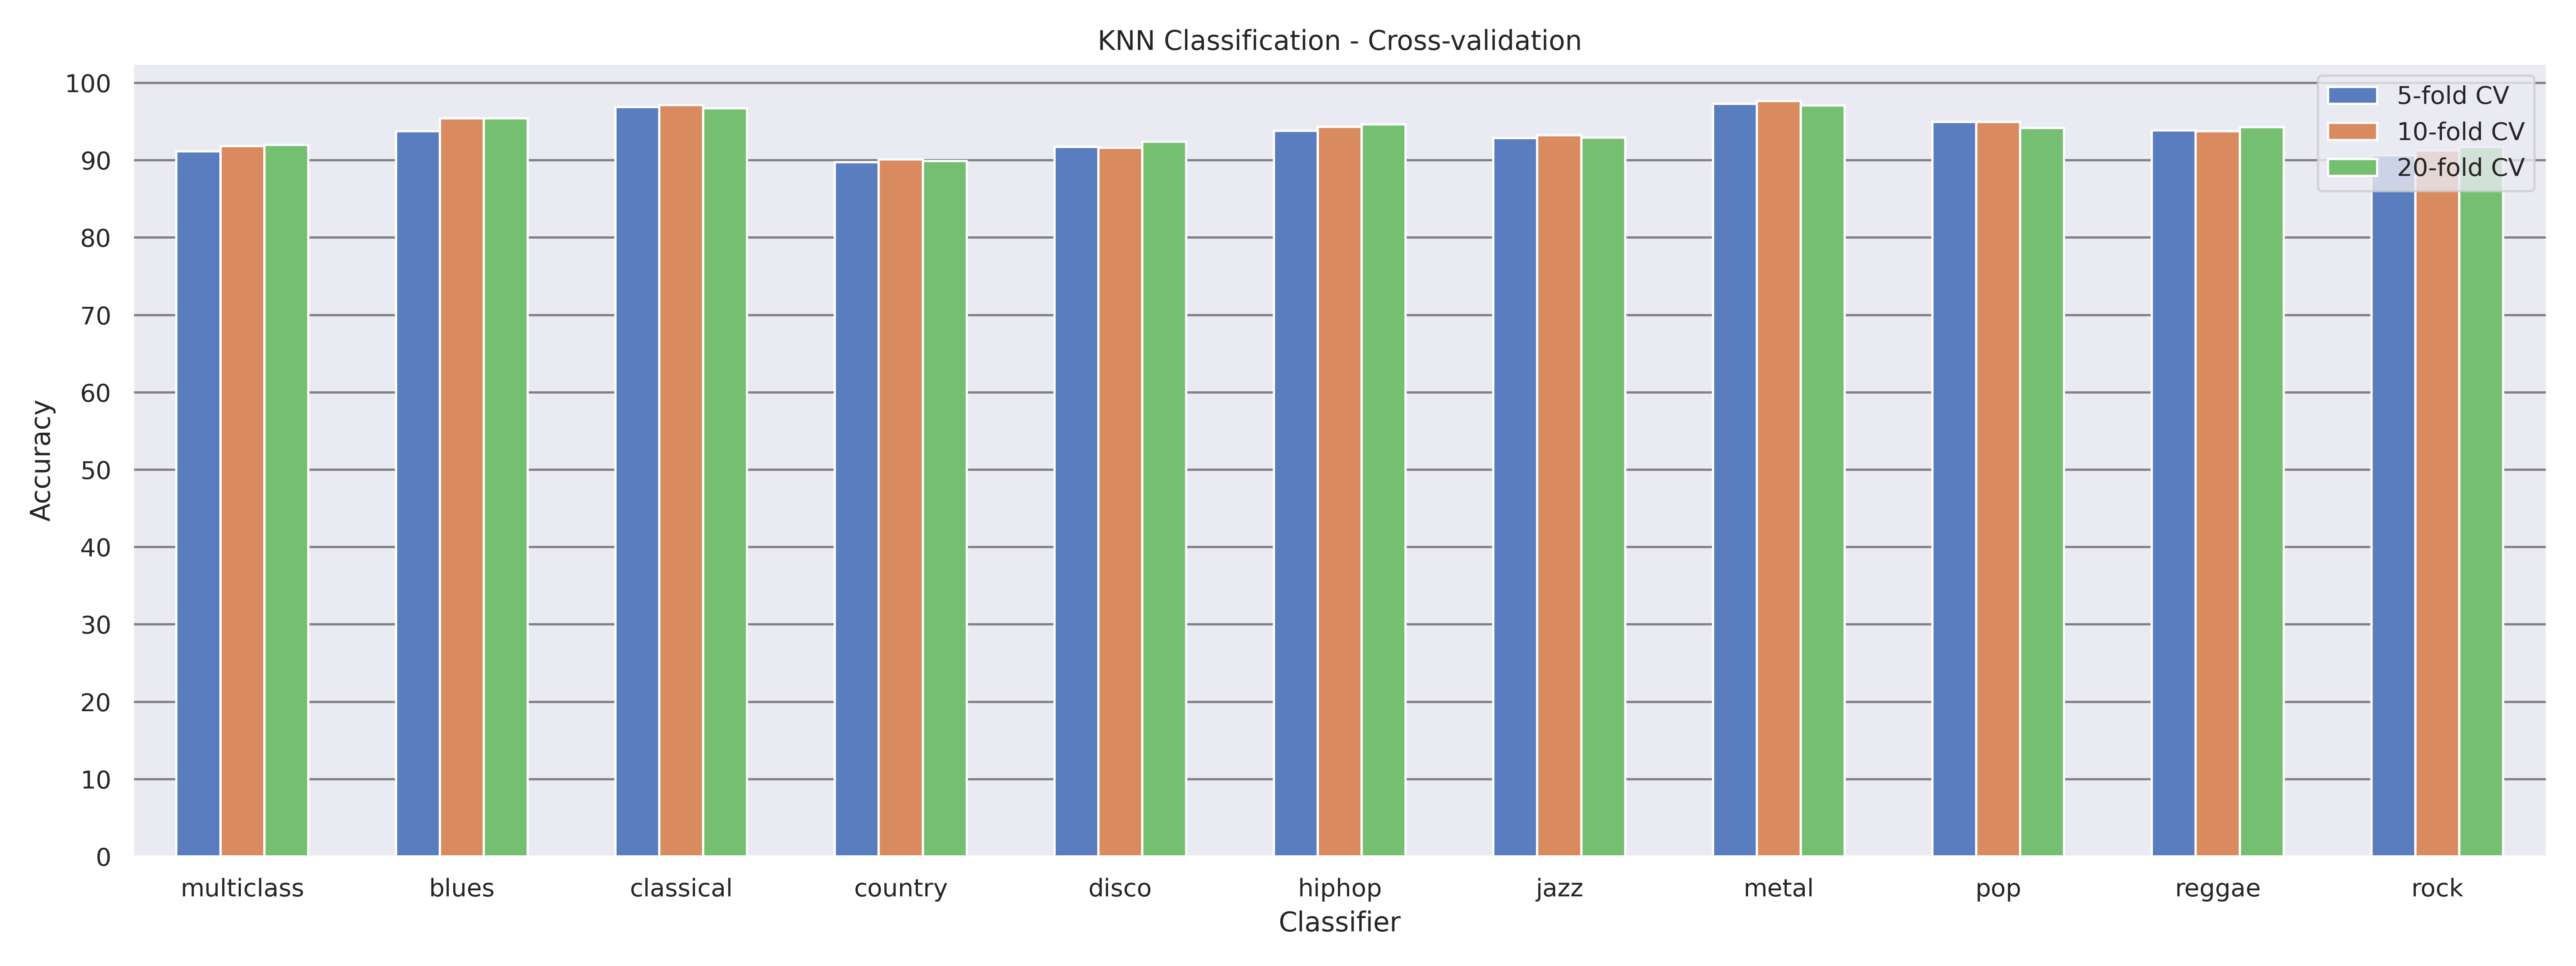
\includegraphics[width=\textwidth]{Figures/knn_d.png}
    \caption{Accuracy of the K-NN classifier with K-fold cross-validation.}
    \label{fig:knnd}
\end{figure}

K-NN was able to reach a very high accuracy. In fact, K-NN is known to be a very powerful model, given that it is also non-parametric and that it makes no assumptions about the data distribution, meaning that is able to capture even very complex relations inside of the data set. It is also known to perform very well when the number of samples is large w.r.t. the number of classes. Its main drawback is that it requires keeping in memory the whole data set in order to compute predictions but in our case, since the data set we are working with is of very small size, this is not an issue.

The following is the confusion matrix of the multi-class K-NN classifier.
\begin{figure}[H]
    \centering
    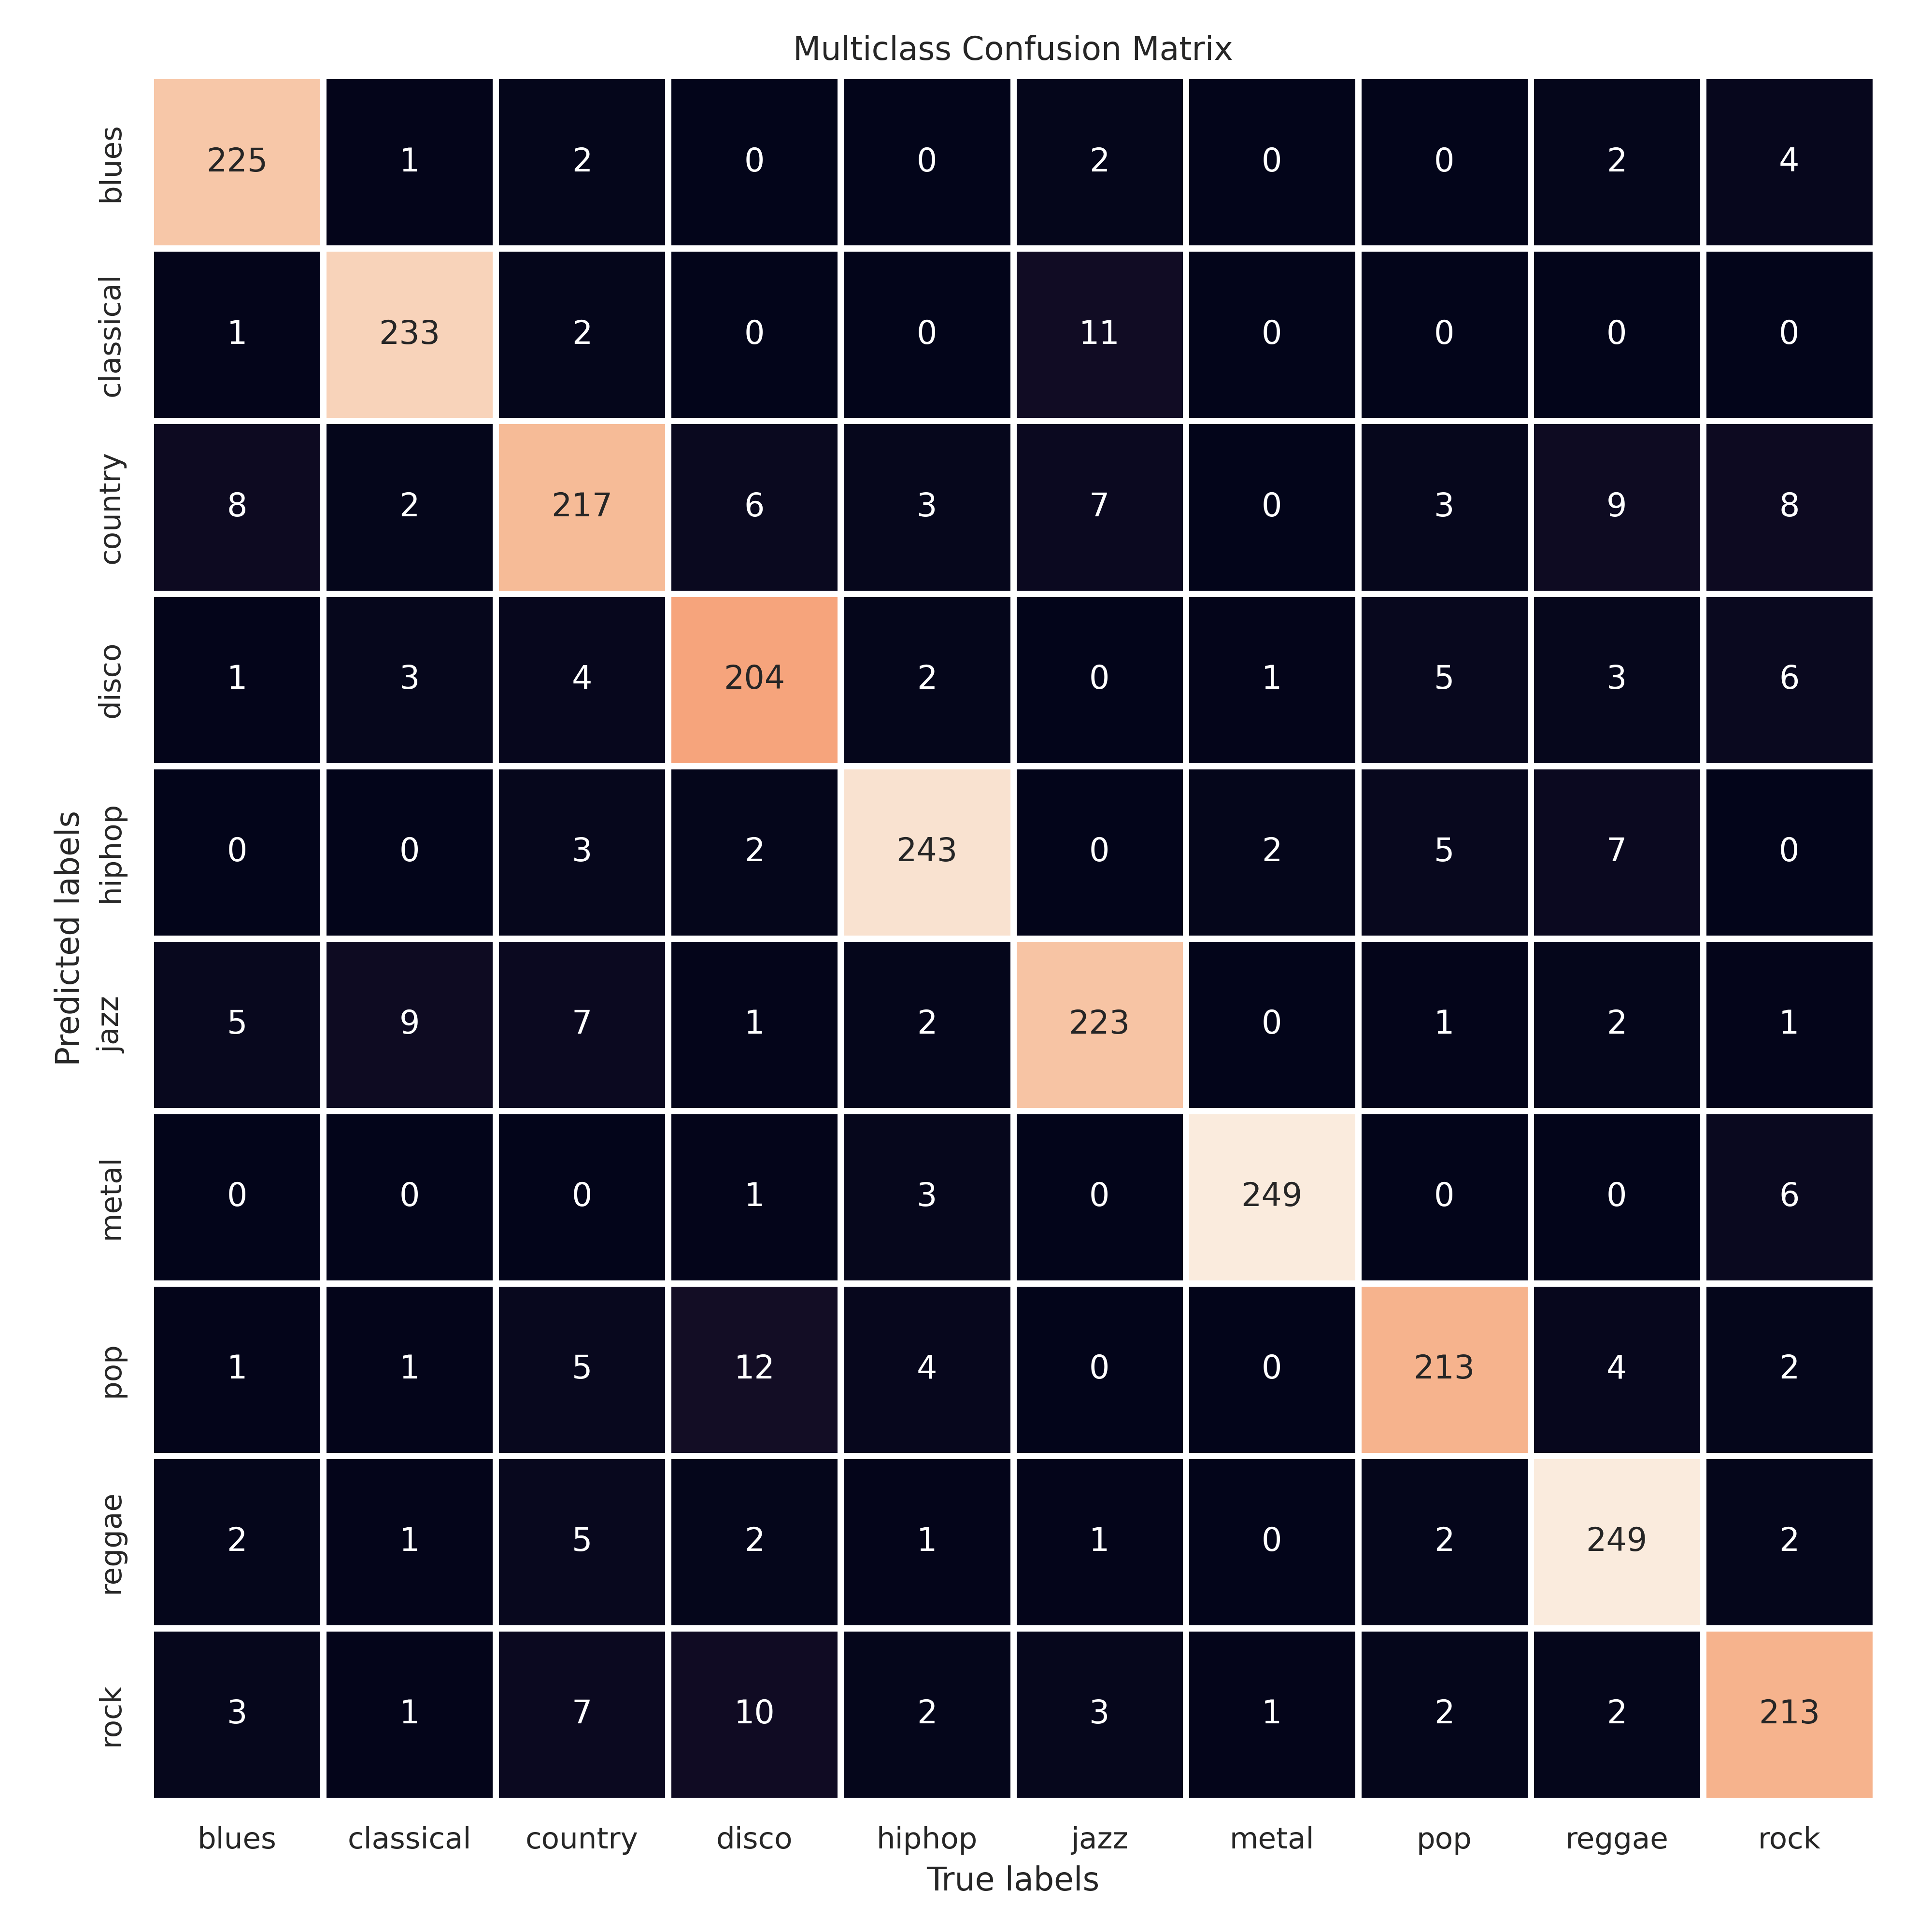
\includegraphics[width=0.7\textwidth]{Figures/knn_m.png}
    \caption{Confusion matrix of the multi-class K-NN classifier.}
    \label{fig:knnm}
\end{figure}


\chapter{Deep Learning models}
\label{ch:dl_models}%
In the last part of our analysis, we will switch from Machine Learning to Deep Learning, exploring a more modern model known as feed-forward fully-connected Neural Networks (FFNNs). Neural Networks are a very powerful instrument and the Universal Approximation Theorem provides a theoretical foundation for their applicability over any problem. 

Fully-connected neural networks are networks in which all the neurons of all layers are connected to all the neurons of the following layer.

For simplicity, in our analysis, we will consider only networks in which all hidden layers have the same amount of neurons. This will let us reduce the number of hyper-parameters that we have to tune, without decreasing the approximation power of the model.

We will need to build and train a different neural network for each one of the classification problems we are facing.


\section{Training}
\label{sec:training}%
This section describes the content of the notebook \textit{NN\_selection.ipynb}. The library used to build, train and evaluate the neural networks is \textit{keras} \cite{chollet2015keras}.

When training a neural network, there is a much larger number of hyper-parameters to be considered w.r.t. ML models, and the time required for the training phase is also much higher. 
In order to find the best model for each one of our problems, we cannot just blindly train a different network for every possible combination of the hyper-parameters: the extremely high number of combinations and the time required to train just one network make this unfeasible. 

Therefore, we will focus on a very small subset of the hyper-parameter space, whose boundaries have been tuned empirically by training pseudo-randomly some hyper-parameter combinations and by checking the performance.

In the multi-class problem, a softmax layer was added after the last layer of the network in order to convert the outputs of the network into probabilities. This network outputs one probability for each class, therefore it has 10 outputs. In the case of the binary problem, the last layer has only one output and uses the sigmoid function as an activation function, in order to map the output in the interval $[0,1]$.

The following ranges were checked:
\begin{table}[H]
    \centering 
    \begin{tabular}{|c | c c  c |}
    \hline
    \rowcolor{bluepoli!40} 
     Hyper-parameter & Start (included) & Stop (included) & Step \T\B \\
    \hline \hline
    Number of hidden layers & 1 & 5 & 1  \T\B \\
    Number of neurons per layer & 15 & 100 & 5   \T\B \\
    Mini-batch size & 5 & 50 & 5   \T\B \\
    \hline
    \end{tabular}
    \\[10pt]
    \end{table}
    
Again, given the large amount of time that the training phase requires, when comparing the performance of two different networks we will not resort to K-fold cross-validation but to a simple train-validation split of the data set, in particular with 80\% of the data allocated for training and the remaining 20\% for testing.

In order to train the networks, the Adam optimizer was used. In the multi-class problem, the loss function used is the categorical cross-entropy, whereas in the binary problem the binary cross-entropy. 
In both cases, the reference metric was the accuracy of the model on the validation set.

This time, other than normalizing the data through standardization, an additional pre-processing step is required: NNs require numerical variables, therefore we will need to convert the \textit{label} from a categorical variable to a numerical variable. In the multi-class case, we need to created a one-hot encoding of such variable, that represents every single label as a vector of $0$ and $1$, where all elements are equal to $0$, except for the one that represents the correct label.
In the binary case, it was enough to encode as $1$ the label of the positive class and as $0$ the label of all the other classes.

Furthermore, we decided to store the results of the evaluation of each possible model in a persistent database, in order to avoid repeating the same training twice and in order to easily filter and aggregate the results with the goal of selecting the best model. The database of choice was \href{https://www.mongodb.com}{MongoDB}, given the extreme flexibility that it allows in storing the data. The connection with the instance of the database was handled with the Python library \href{https://www.mongodb.com/docs/drivers/pymongo/}{\textit{pymongo}}.

At the beginning of the training phase, we query the database in order to check if a network with the current combination of hyper-parameters had already been trained. If yes, the training phase is aborted and the loop restarts with a different combination of hyper-parameters. Otherwise, the training phase is performed and at the end, the accuracy of the trained model, together with the combination of its hyper-parameters, is stored in the database.

The following table reports the hyper-parameters of the models selected at the end of this phase.

\begin{table}[H]
    \centering 
    \begin{tabular}{|c | c c c |}
    \hline
    \rowcolor{bluepoli!40} 
     Classification problem & Number of hidden layers & Neurons per layer  & Batch size \T\B \\
    \hline \hline
    multi-class & 2 & 95 & 5  \T\B \\
    blues & 1 & 75 & 5   \T\B \\
    classical & 1 & 60 & 15   \T\B \\
    country & 1 & 80 & 20   \T\B \\
    disco & 2 & 65 & 5   \T\B \\
    hip-hop & 1 & 25 & 15   \T\B \\
    jazz & 2 & 55 & 30   \T\B \\
    metal & 2 & 70 & 15   \T\B \\
    pop & 2 & 60 & 50   \T\B \\
    reggae & 1 & 90 & 25   \T\B \\
    rock & 1 & 75 & 20   \T\B \\
    \hline
    \end{tabular}
    \\[10pt]
\end{table}

With every network, the activation function used was the SELU (Scaled Exponential Linear Unit) which is an improved version of the very well-known ReLU (Rectified Linear Unit). Different activation functions were considered in this phase, mainly the hyperbolic tangent, the ReLU, the ELU (Exponential Linear Unit) and the SELU. The latter was found to be the best-performing one and therefore was kept.

In the last section of the \textit{NN\_selection.ipynb} notebook, we are retrieving the best combinations of hyper-parameters selected from the database through the id associated with their entry, in order to save those models using the \textit{model.save} method of \textit{keras}, which stores the all the information required to transfer the model from one notebook to another in just a single file in the \textit{h5} format. 

In this way, we will be able to evaluate the performance of those models in another notebook, without the need of connecting to the database at every single step.
All the models can be found in the \textit{models} folder of the GitHub repository \cite{project-repository}.

\section{Evaluation}
\label{sec:eval}%
As anticipated, the evaluation of the selected models is carried out in a different notebook, which is \textit{NN\_classification.ipynb}. In this notebook, we are loading the models saved in \textit{NN\_selection.ipynb} through the use of the \textit{load\_model} function from \textit{keras}. We want to train those models once again, but with the same methodologies (i.e. train-validation split and K-fold cross-validation) used for ML models, in order to allow for a fair comparison between them.

In the following charts, we can see the accuracy of the multi-class classifier and of the binary classifiers with different sizes of the train-validation split and with a different number of folds for the K-fold cross-validation. The models we are using are the ones with the hyper-parameters selected in the previous step.

\begin{figure}[H]
    \centering
    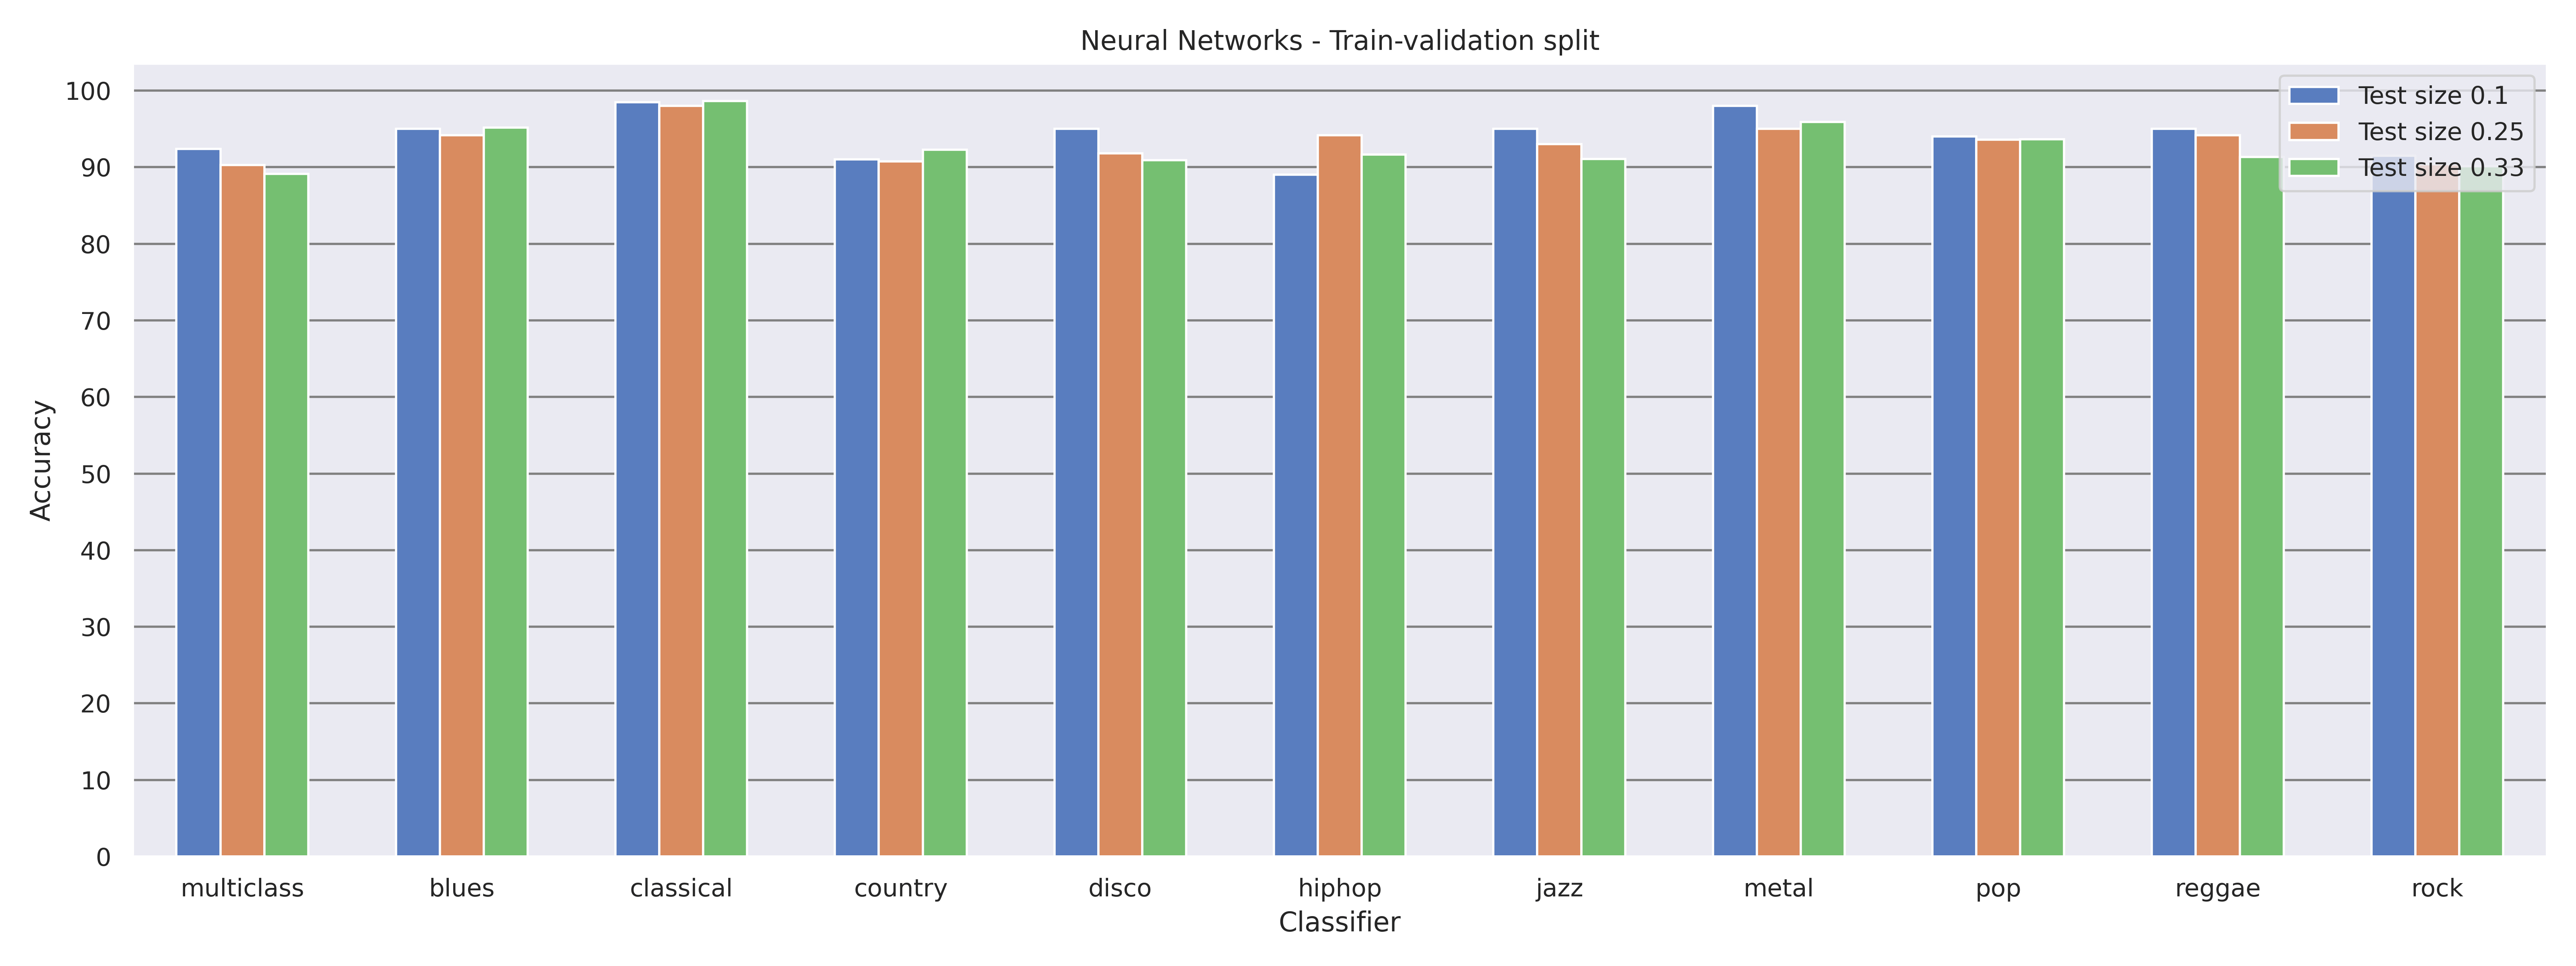
\includegraphics[width=\textwidth]{Figures/nn_s.png}
    \caption{Accuracy of the NN classifier with the train-validation split.}
    \label{fig:nns}
\end{figure}

\begin{figure}[H]
    \centering
    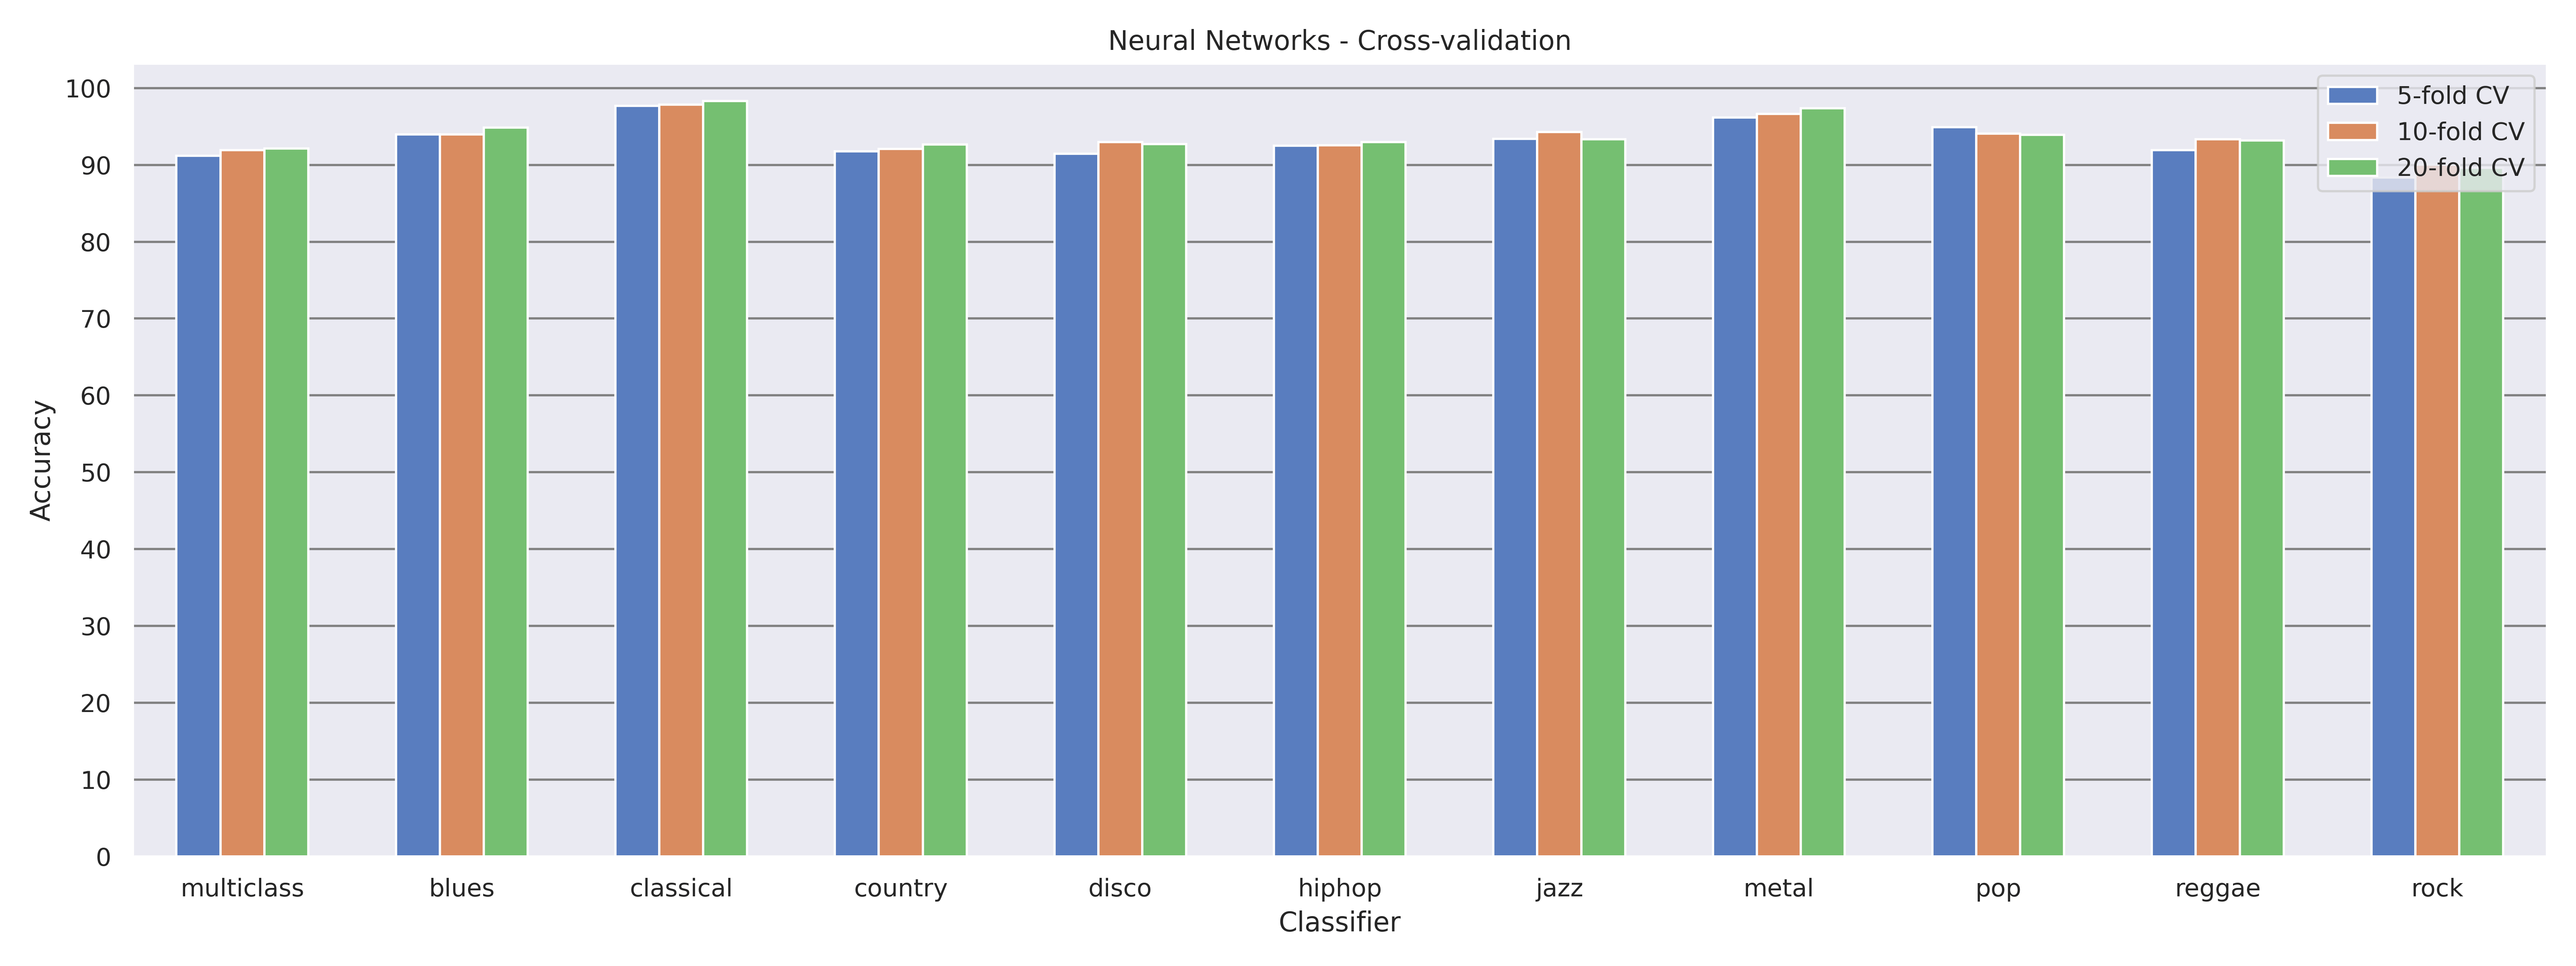
\includegraphics[width=\textwidth]{Figures/nn_d.png}
    \caption{Accuracy of the NN classifier with K-fold cross-validation.}
    \label{fig:nnd}
\end{figure}

As expected, the selected NNs achieved very high accuracy in all the problems.
In fact, NNs are capable of learning any complex patterns and relationships in the data. 
However, even if they offer very high performance, they suffer from many drawbacks, such as their long training phase, the very large amount of data they require and their lack of interpretability, being a Black-Box model.

The following is the confusion matrix of the multi-class NN classifier.

\begin{figure}[H]
    \centering
    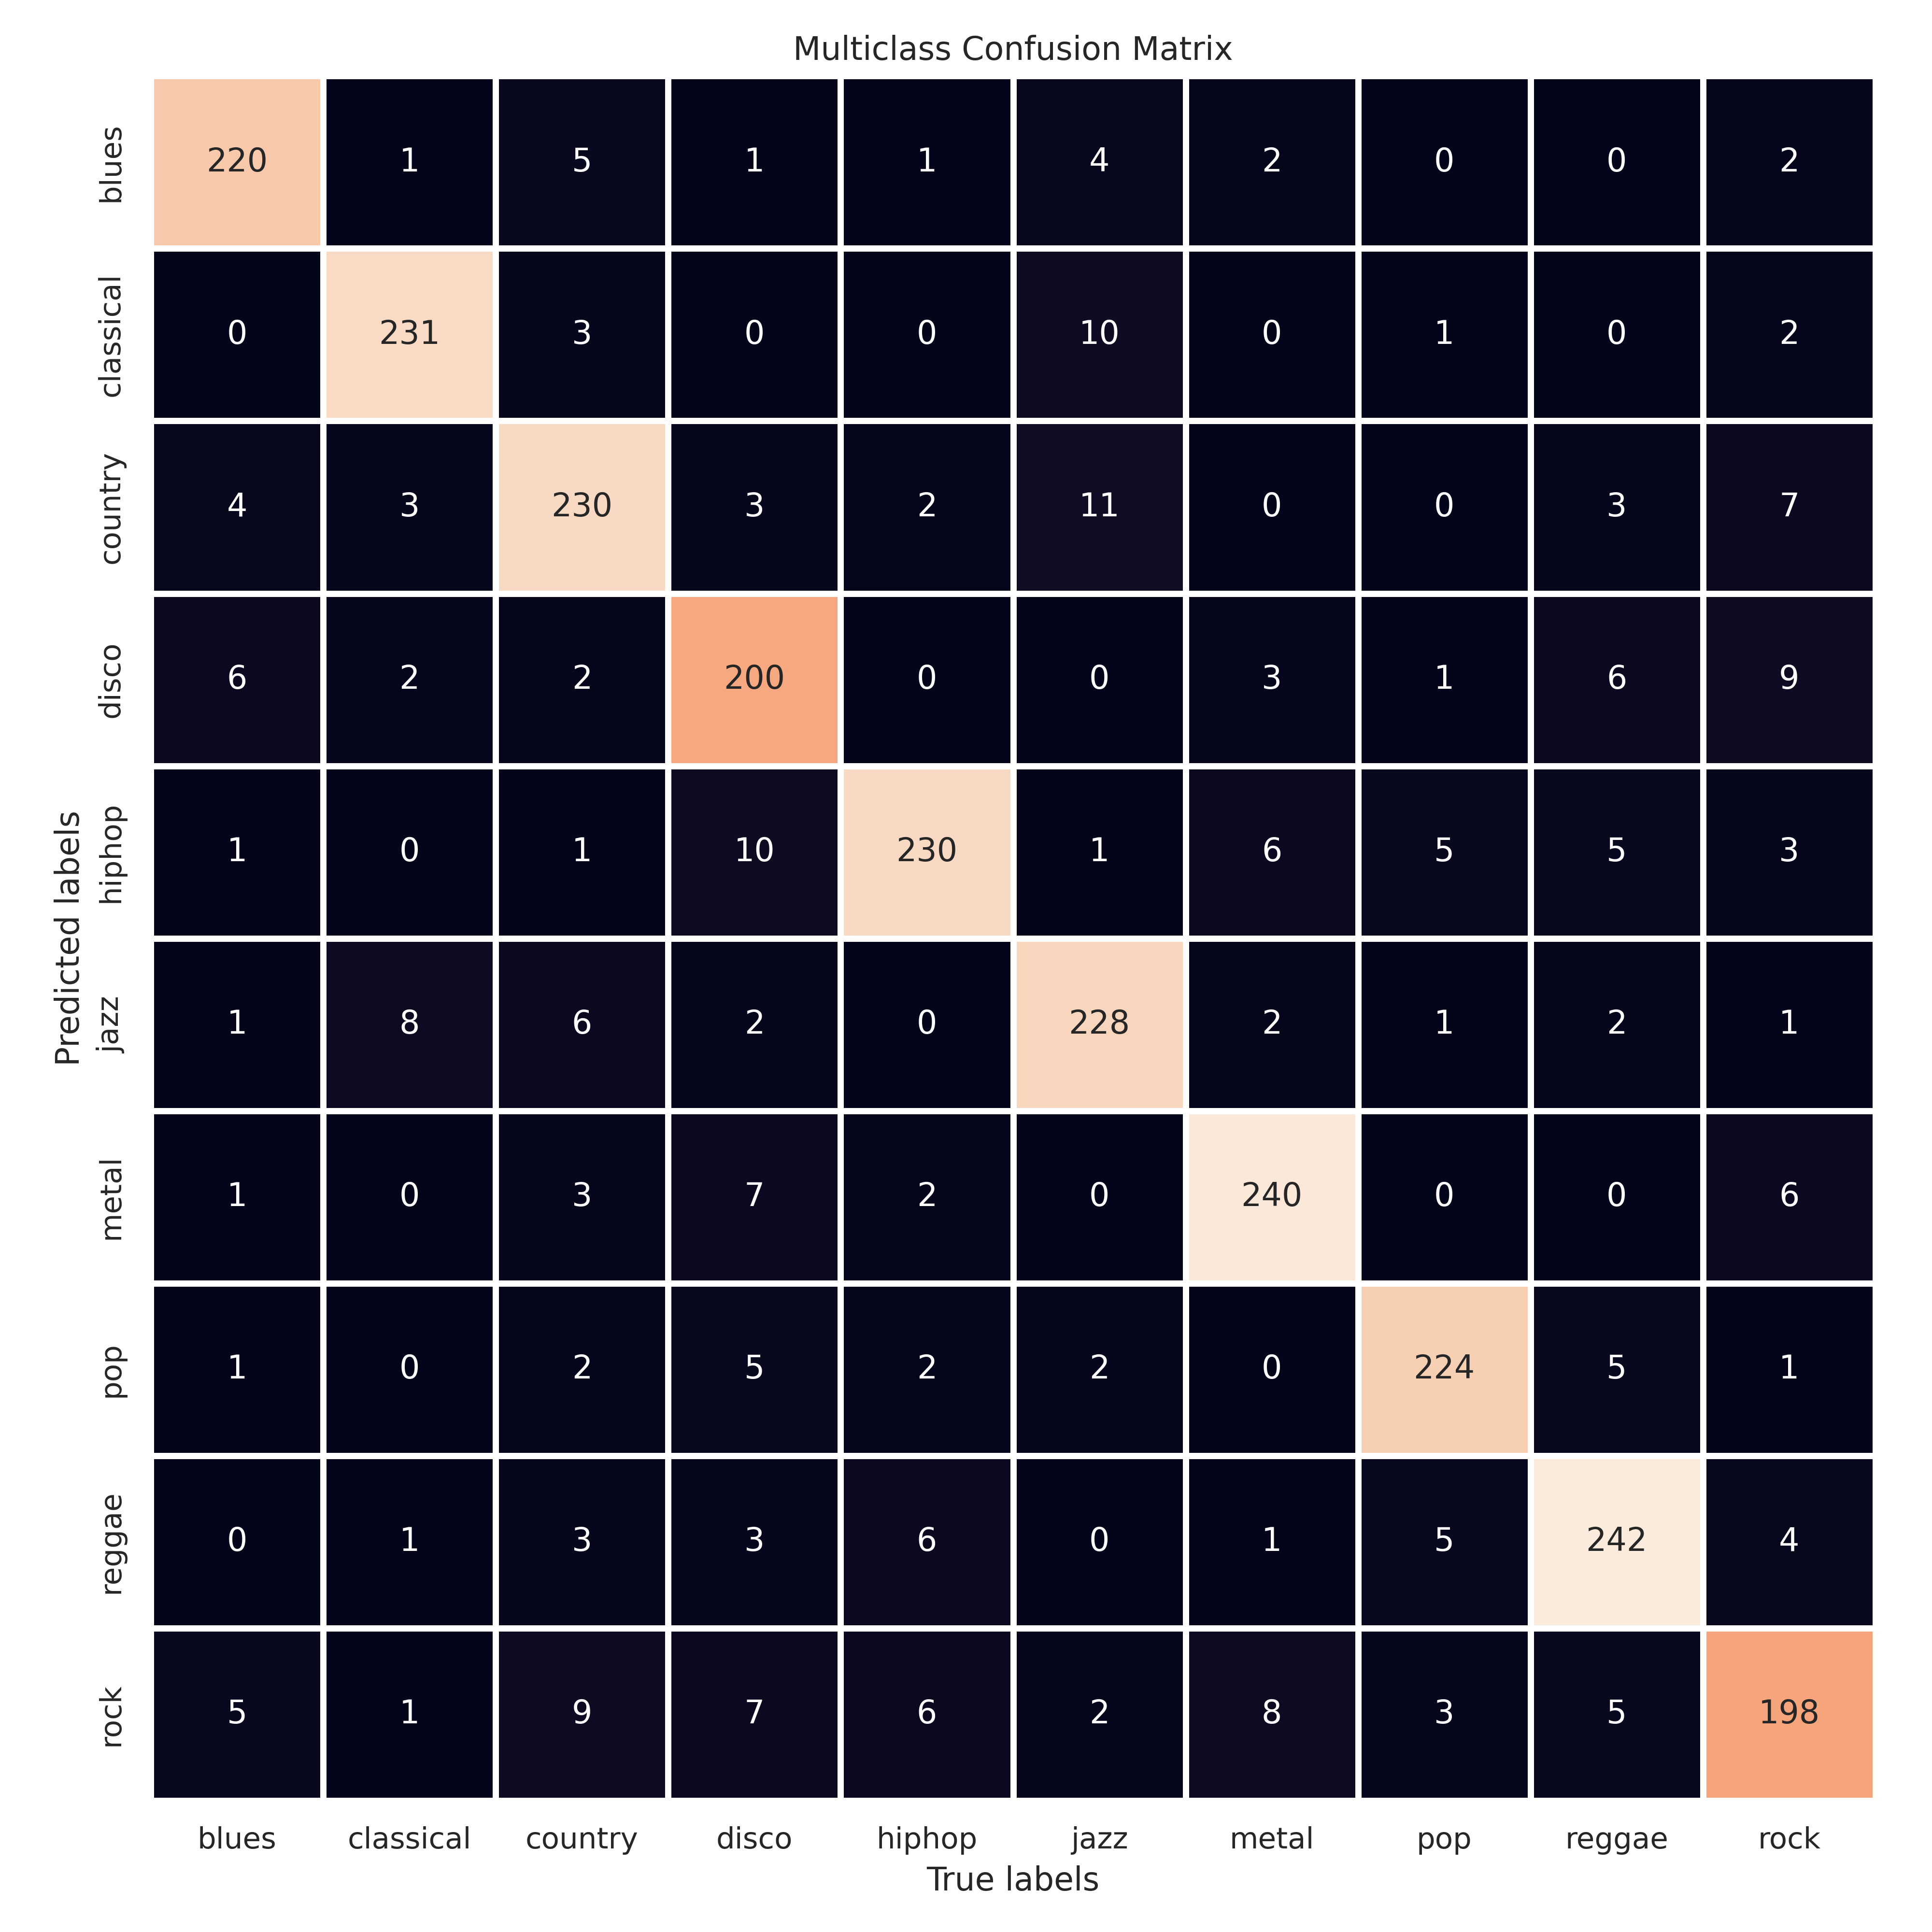
\includegraphics[width=0.7\textwidth]{Figures/nn_m.png}
    \caption{Confusion matrix of the multi-class NN classifier.}
    \label{fig:nnm}
\end{figure}

\chapter{Comparison}
\label{ch:comparison}%
In the following chart, we can see a comparison of the accuracy of all the models considered in this project, both in the multi-class case and in the binary case.
Those results were produced by evaluating all the models using 20-fold cross-validation.

\begin{figure}[H]
    \centering
    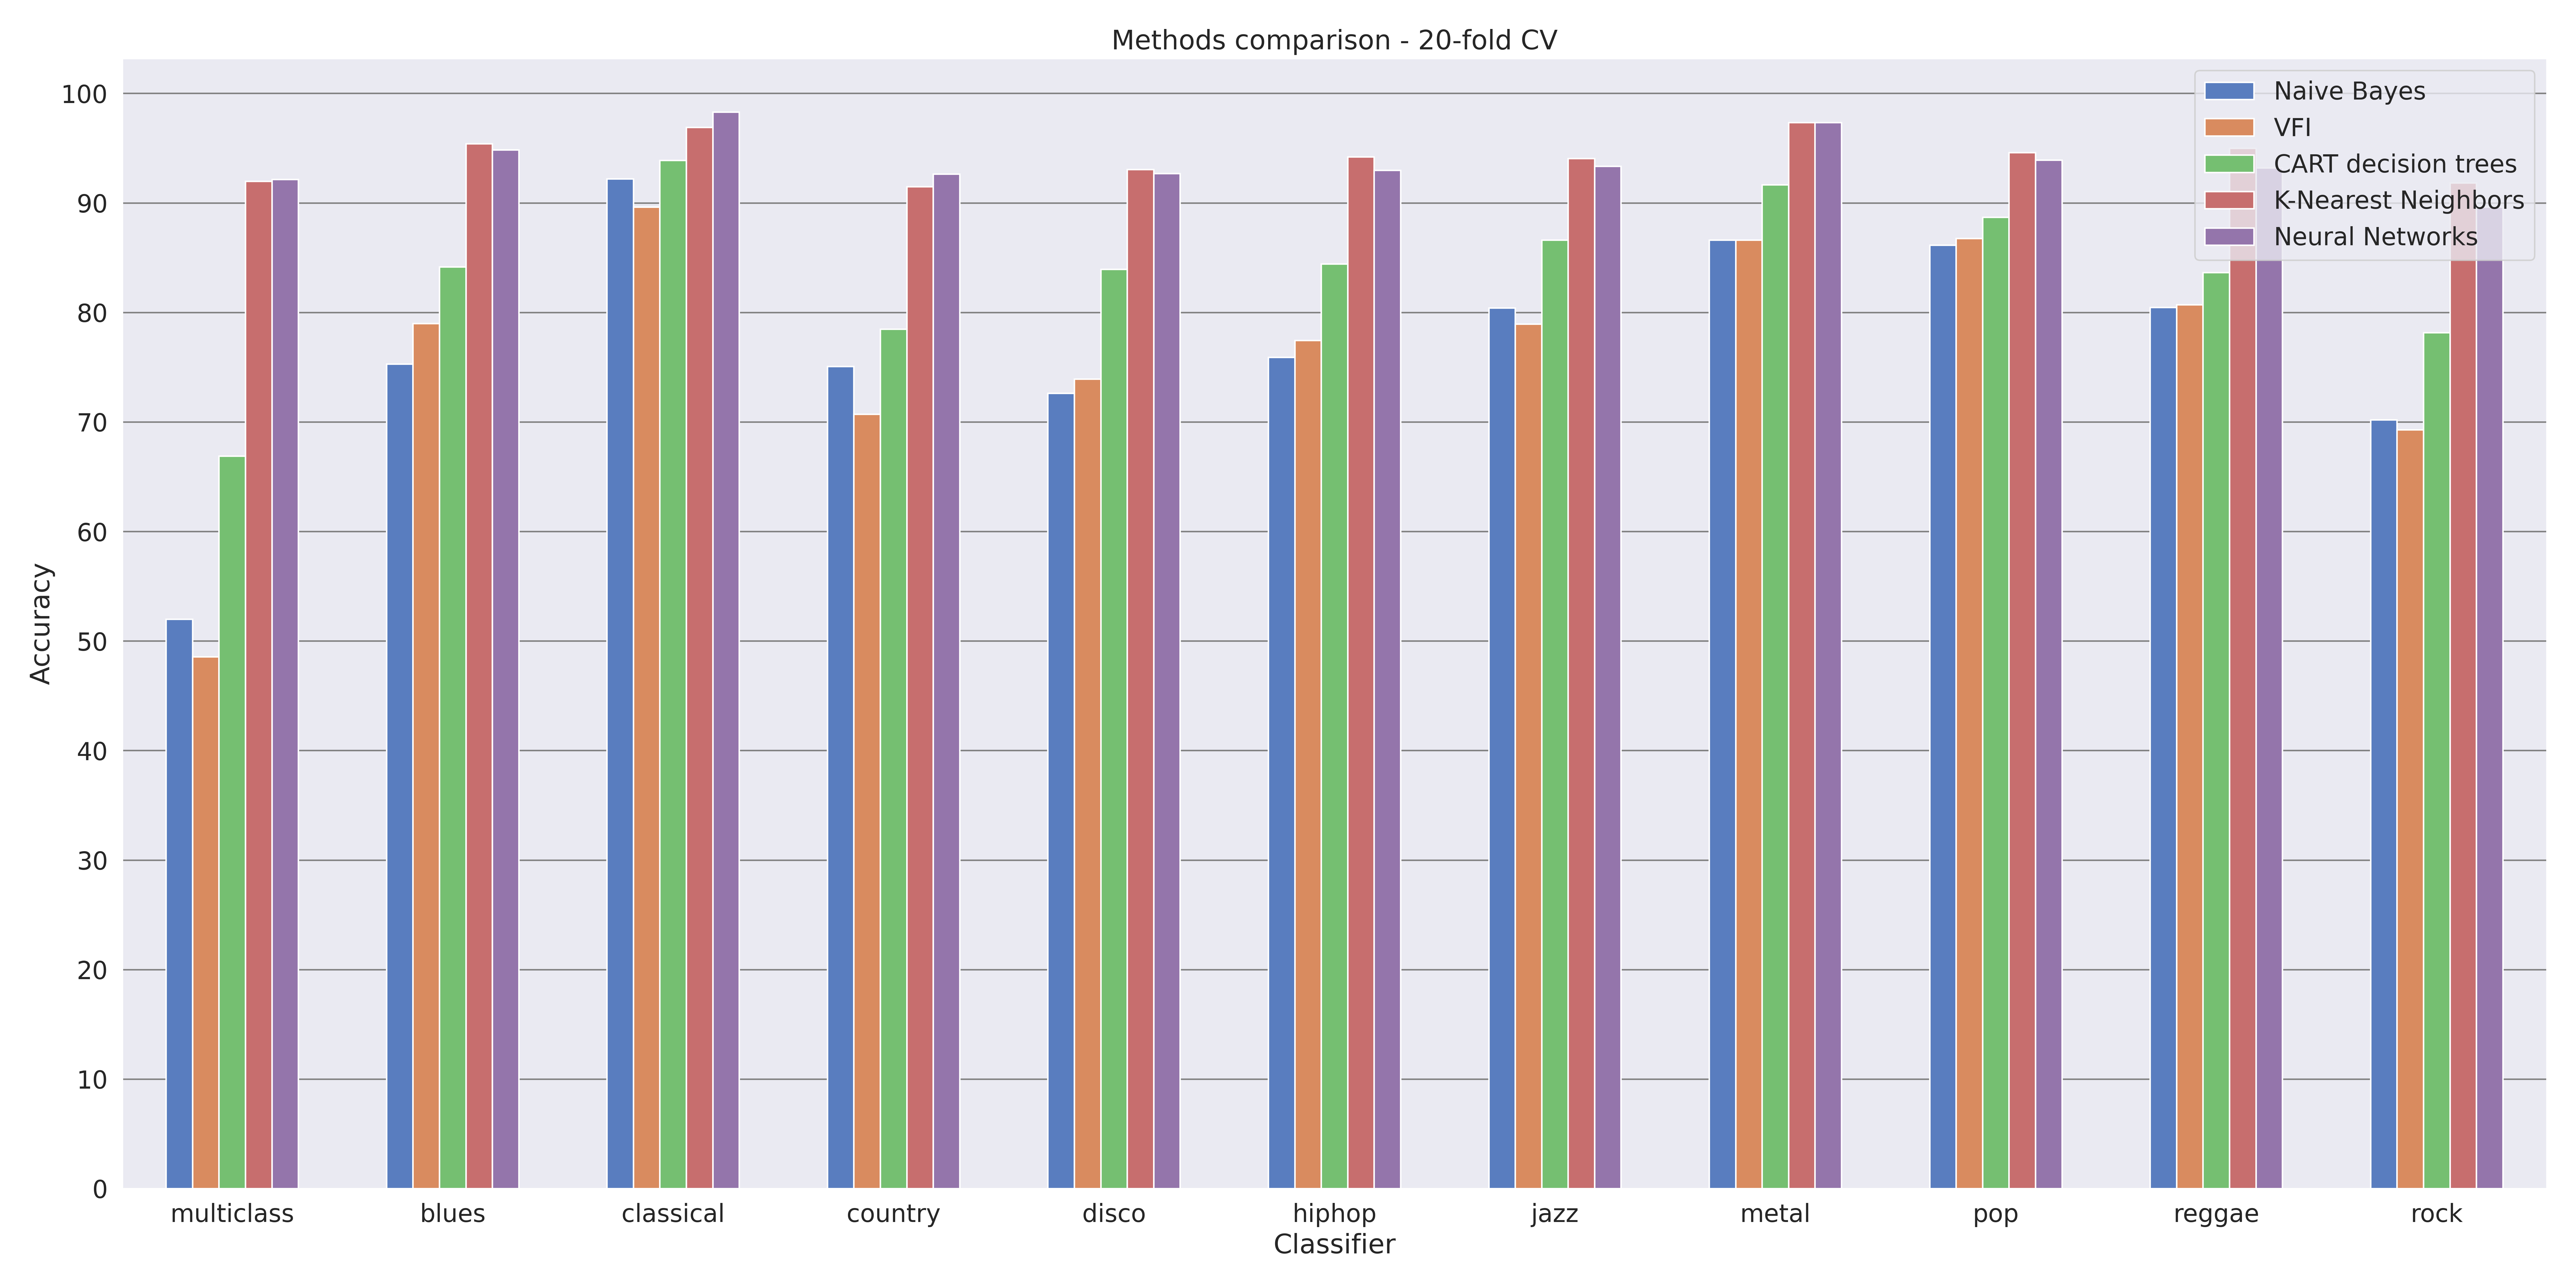
\includegraphics[width=\textwidth]{Figures/comparison.png}
    \caption{Comparison of the accuracy of the models considered in the project.}
    \label{fig:comp}
\end{figure}

As expected, K-Nearest Neighbors (K-NN) and Neural Networks (NNs) are the most performing models. On the other hand, the performance of very simple models like Naive Bayes (NB) and Voting Feature Interval (VFI) is much worse, in particular in the more complex setting of the multi-class classification problem.

An interesting remark is that we expected more performance from NNs, given their theoretical properties. However, we have to cope with the fact that we are in a real-world setting, in which the data at our disposal is not unlimited. NNs and Deep Learning models, in general, are known to require much more data than Machine Learning models. Even if we were able to extend the number of samples in the data set from $1000$ to $10000$ by splitting each song into 10 tracks with a length of 3 seconds, we cannot say that we have enough data to effectively train a Deep Learning model. It is possible that this is the reason why we are getting a high performance indeed but still not completely outperforming a simpler model like K-NN.

On the other hand, as stated in the original paper \cite{original-paper}, binary classification models outperform multi-class classification models in terms of accuracy. The task of separating musical instances of a particular genre from all the others  seems easier.

Furthermore, from an analysis of the performance in the binary problems, we can see that some musical genres are much harder to recognize w.r.t. other genres. For instance, we can see that telling whether a musical track resembles classical music or not is an easy task given that all models, even the least powerful ones, were able to achieve high accuracy. On the other hand, the rock genre seems to be hard to classify and we have to resort to more powerful models in order to get good results. 

This is expected since some genres are characterized by an inherent mutual ambiguity, meaning that it is sometimes hard, even for human annotators, to tell the difference between them. This is the case of genres like blues and jazz. The paper \textit{Browsing Music Spaces: Categories And The Musical Mind} \cite{music-paper}  states that "Genres emerge as terms, nouns that define recurrences and similarities that members of a community make pertinent to identify musical events". Therefore, we can say that musical genres are in general hard to be systematically described and no complete agreement exists in their definition and assessment. 


\chapter{Conclusions and future developments}
\label{ch:conclusions}%
The ambiguity inherent to every definition of musical genre, together with the high dynamics that undermine its persistence over time, characterizes the complexity of the automatic genre categorization task. Nonetheless, as stated in the original paper \cite{original-paper}, the results we obtained are very encouraging and suggest that simple musical features can provide effective information for genre categorization. We can conclude that building systems for automatic genre categorization is certainly possible and can also bring a high level of accuracy. 

The project can be developed further in two different directions:

\begin{itemize}
    \item As suggested in the original paper, we can collect the binary classifiers into a hierarchical meta-learner, whose performance is expected to be better than the performance of the corresponding multi-class classifier.
    \item Starting from the audio tracks, we could extract their corresponding spectrogram, which is a very compact representation of the audio track in the form of an image that allows us to see how the frequencies vary over time. Given that the spectrogram is an image, we can process it using more modern technologies from Deep Learning, like Convolutional Neural Networks (CNNs). In that case, we would also be able to increase the samples at our disposal using a technique called data augmentation, which consists in fictitiously augmenting the data set by performing geometrical transformations on the images. Given those premises, we expect that CNNs will guarantee even more performance w.r.t. fully-connected NNs.
\end{itemize}

%-------------------------------------------------------------------------
%	BIBLIOGRAPHY
%-------------------------------------------------------------------------

\addtocontents{toc}{\vspace{2em}} % Add a gap in the Contents, for aesthetics
\bibliography{Thesis_bibliography} % The references information is stored in the file named "Thesis_bibliography.bib"

\cleardoublepage

\end{document}
